%%% stat_interpretation
\label{ch:stat_interpretation}

In this chapter, we outline our fitting approach and present the main results of the fit. 
Our goal is to measure the signal strength ($\mu_{VBS}$) of the EW $VV$+jj production within the VBS-enhanced phase space for the 1-lepton channel, 
using a DNN method. 
Detailed discussions will be provided in Section~\ref{sec:Fit_Results_ub}.

The fit model is constructed using MC-based templates for both the signal and background processes. In addition to estimating the primary parameters of interest (POIs), the model aims to constrain the normalization of the predominant background processes, specifically \Wjets and \ttbar production, using dedicated control CRs established in earlier chapters. Minor backgrounds, such as $VV$ and single-top processes, are adjusted using priors, with specific extrapolation parameters derived for them. The model incorporates the main sources of systematic uncertainties, applying normalization and/or shape effect schemes as appropriate. 
%The approach to de-correlating these uncertainties will be detailed in Section \ref{subsec:fit_options}.

%%%
\clearpage
\section{Introduction}
\label{sec:mll_def}

To determine the signal strength parameter $\mu$ ($\mu_{VBS}$), a binned maximum likelihood fit is used in the statistical analysis. The likelihood function is formulated as follows:
\begin{equation} \label{eq:Lh1}
	\mathcal{L}(N, \tilde{\theta} | \mu, \theta) = \mathrm{Pois}\,(\mu | \mu s + b) \cdot p(\tilde{\theta} | \theta)
\end{equation}
Here, $\mathrm{Pois}\,(\mu | \mu s + b)$ represents the product of Poisson probability terms across all histogram bins:
\begin{equation} \label{eq:Lh2}
	\mathrm{Pois}\,(\mu | \mu s + b) = \prod_{i=1}^{N_{\text{bins}}} \frac{(\mu s_{i}(\theta) + b_{i}(\theta))^{N_{i}} e^{- (\mu s_{i}(\theta) + b_{i}(\theta))}}{N_{i}!}
\end{equation}
In this formulation, $\mu s_{i}$ and $b_{i}$ denote the expected numbers of signal and background events in bin $i$, respectively, while $N_{i}$ represents the number of observed events in that bin. The second part of Equation \ref{eq:Lh1}, $p(\tilde{\theta} | \theta)$, typically referred to as the prior, incorporates our knowledge about the systematic effects considered in the analysis. This binned likelihood approach allows for a robust estimation of $\mu$ while accounting for various statistical and systematic uncertainties.

%%%
%The statistical analysis uses a binned maximum likelihood approach, formulated as a product of Poisson probability terms to evaluate the data. The likelihood function is represented by:
%
%\begin{equation}
%\mathrm{Pois}\,(n|\mu S+B)\left[ \prod_{b\in \text{bins}}^{n} \frac{\mu \nu^{\mathrm{sig}}_{b}+\nu^{\mathrm{bkg}}_{b}}{\mu S+B} \right],
%\end{equation}
%
%In this equation, $\mu$ is the signal strength parameter that scales the expected signal yield $\nu^{\mathrm{sig}}_b$ in each histogram bin $b$. 
%The term $\nu^{\mathrm{bkg}}_b$ indicates the expected background contribution in the same bin.

The sensitivity of the signal and background predictions to systematic uncertainties is quantified through nuisance parameters (NPs), denoted as $\theta$. 
These NPs are typically modeled using either Gaussian or log-normal distributions, with log-normal priors being preferred for normalization uncertainties to ensure that the likelihood remains positive. The expected counts of signal and background events in each bin are modeled as functions of $\theta$. This modeling is structured so that event rates across different categories exhibit a log-normal behavior when $\theta$ is governed by normal distributions.

Priors are used to constrain the NPs towards their nominal values within their assigned uncertainties. This is achieved by incorporating penalty terms or auxiliary measurements into the likelihood function. These additions cause the likelihood to increase whenever an NP deviates significantly from its nominal value. Consequently, the likelihood function $\mathcal{L} (\mu,\theta)$ depends on both the signal strength parameter $\mu$ and the NPs $\theta$. This setup facilitates the integration of our understanding and uncertainties about the system into the analysis, ensuring that the estimation of $\mu$ is consistent with the prior knowledge encapsulated in $\theta$.

The nominal fit result, in terms of the signal strength parameter $\mu$ and its uncertainty $\sigma_{\mu}$, is determined by maximizing the likelihood function across all parameters. This process yields the maximized log-likelihood value (MLL).




%%%
%%\subsection{Unblinding strategy}
\label{sec:fit_unbliding_str}

We aimed an unblinding procedure to take into account the different aspects of the analysis.
The analysis is designed as a search both for the SM EW VV+jj processes both for the aQGC interpretation, 
so, we want to keep sensitive regions blinded and not use data in fit validation.
On the other hand, we want to make sure our ML discriminant has good modelling and avoid the need to have strong constraints or pulls after the unblinding.
Therefore, we designed the procedure to have:

\begin{itemize}
  \item model inspections and validation
  \item fit on data as much as possible close to the sensitive region but keeping the sensitive region completely blinded
\end{itemize}

In the following we will refer to 'left-side' or 'leftmost side' of the SR discriminant distribution 
as the bins in the SR that are less sensitive to the signal. In particular, we use a fixed signal threshold 
to define them, as explained in the following, and we also checked that signal significance is negligible
in those bins.

The procedure is the following:

\underline{Preliminary}:

\begin{itemize}
\item each variable is unblinded already in CRs
\item for conditional fits, 
  \begin{itemize}
    \item we can rely on EW VV+jj fully leptonic measurements, they observed $\mu \sim 1.5$
    \item this is the preference but it should not matter too much if we stay in the left-side only of the SRs
  \end{itemize}
\end{itemize}
  
\underline{Discriminant distribution [SR]}:

\begin{itemize}
  \item the binning results from Transformation-D; parameters of the transformation used are (10,5), 
        this is a good starting point and we are currently using this setup for the results shown in this section.
  \item split the SR in left/right-sides:
    \begin{itemize}
      \item the rightmost bins contain 75\% of the signal.
      \item the leftmost bins contain 25\% of the signal.
      \item since these 25\%/75\% will not match exactly a bin boundary, the criterion is to keep rather fewer than more leftmost bins.
    \end{itemize}
    \item unblind the left-side of the distribution only
    \item the right side is kept blinded and excluded from both Data/MC plots and fitting for now
\end{itemize}

\underline{Fit strategy with left-side unblinded}:
\begin{itemize}
  \item Step 0: Asimov fit over the full range.
  \item Step 0+: global data fit in CRs (this is shown in Appendix \ref{app:CROnlyFits}).
  \item Step 1: Asimov fit restricted to the leftmost bins.
  \item Step 2: Global data fit restricted to the leftmost bins.
    \begin{itemize}
      \item investigate whether all pulls and constraints are justified. 
    \end{itemize}
      %\item we could try unconditional as well, but we should check the actual significance of the left-side bins
  {\color{gray}
  \item Step 3: %(assuming it is good what we see so far):
    [we designed this step as well in the main model inspection strategy but then we decided to post-pone it]
  \begin{itemize}
      \item adjust the background (and signal) model according to the floating normalizations and NP pulls determined in Step 2.
      \item build hybrid data: real data in the leftmost bins, Asimov SM (bkg+signal) in the rightmost bins
      \item evaluate the signal significance 
      \item conditional Global fit over the whole range
    \end{itemize}
  }
\end{itemize}


Figure \ref{fig:RNN_SoB_nJets5} shows the score distributions in the 9 SRs; 
in particular, the ratio panels show some estimator of the signal contribution, 
like the signal efficiency (blue) and the SoB in each bin (orange). 
They give a feeling of the most sensitive bins and they have been used to fine-tune the un-blinding strategy in the SR. 
The SoB(<0.05) seems to be too aggressive, then a fixed signal efficiency threshold has been used. 
Furthermore, since the final discriminant has been slightly updated towards final results 
the threshold has been increased to 75\% to avoid undesired un-blinding in the border region.
Now, the results shown are with the latest and frozen discriminant setup.

%%% SoB plots
\begin{figure}[ht]
      \centering
       \subfigure[\emph{\zlep, Resolved SR}]{\includegraphics[width=0.3\textwidth]{figures/ml_analysis/RNN_SoBPlots/SoB/0lep/nJets5/PlotAsySig_EWZVjj-1.pdf}}
       \subfigure[\emph{\zlep, Merged HP SR}]{\includegraphics[width=0.3\textwidth]{figures/ml_analysis/RNN_SoBPlots/SoB/0lep/nJets5/PlotAsySig_EWZVjj-2.pdf}}
       \subfigure[\emph{\zlep, Merged LP SR}]{\includegraphics[width=0.3\textwidth]{figures/ml_analysis/RNN_SoBPlots/SoB/0lep/nJets5/PlotAsySig_EWZVjj-3.pdf}} \\

       \subfigure[\emph{\olep, Resolved SR}]{\includegraphics[width=0.3\textwidth]{figures/ml_analysis/RNN_SoBPlots/SoB/1lep/nJets5/PlotAsySig_EWWVjj-1.pdf}}
       \subfigure[\emph{\olep, Merged HP SR}]{\includegraphics[width=0.3\textwidth]{figures/ml_analysis/RNN_SoBPlots/SoB/1lep/nJets5/PlotAsySig_EWWVjj-2.pdf}}
       \subfigure[\emph{\olep, Merged LP SR}]{\includegraphics[width=0.3\textwidth]{figures/ml_analysis/RNN_SoBPlots/SoB/1lep/nJets5/PlotAsySig_EWWVjj-3.pdf}} \\

       \subfigure[\emph{\tlep, Resolved SR}]{\includegraphics[width=0.3\textwidth]{figures/ml_analysis/RNN_SoBPlots/SoB/2lep/nJets5/PlotAsySig_EWZVjj-1.pdf}}
       \subfigure[\emph{\tlep, Merged HP SR}]{\includegraphics[width=0.3\textwidth]{figures/ml_analysis/RNN_SoBPlots/SoB/2lep/nJets5/PlotAsySig_EWZVjj-2.pdf}}
       \subfigure[\emph{\tlep, Merged LP SR}]{\includegraphics[width=0.3\textwidth]{figures/ml_analysis/RNN_SoBPlots/SoB/2lep/nJets5/PlotAsySig_EWZVjj-3.pdf}} \\

       \caption{[nJets5 models] Score distributions for the MC predictions of the SM bkg and the EW VV+jj process for the 9 SRs. The ratio panel shows the integrate signal efficiency starting from the left side (blue), the local SoB in each single bin (orange) and the cumulative SoB starting from the left side (green).}
       \label{fig:RNN_SoB_nJets5}
\end{figure}

%%% Local Variables:
%%% mode: latex
%%% TeX-master: "../../ANA-STDM-2018-27-INT1"
%%% End:

%%%
\clearpage
\section{Fit inputs and options}
\label{subsec:fit_options}

%For the statistical interpretation, we utilize outputs from the CxAODReader framework, providing histograms of relevant distributions within designated regions to the WSMaker statistical framework for this analysis. 
%\mbox{\texttt{\href{https://gitlab.cern.ch/atlas-physics/sm/ew/vbs-semileptonic-run2/WSMaker\_VBSVV}{WSMaker\_VBSVV}}}
%statistical framework for this analysis.

For the statistical interpretation, we utilize outputs from the CxAODReader framework, which provides histograms of relevant distributions within designated regions. These histograms are then supplied to the WSMaker statistical framework for this analysis.

In the fitting stage of the analysis, the relevant variables include the \mjjtag and the final DNN score distributions. Table~\ref{tab:fitregions_1lep} summarizes the regions and variables used in the fit of the analysis. These regions are simultaneously fitted using a binned profile likelihood method to extract the parameter of interest (POI), which, for the Standard Model measurement, is the signal strength of the EW VBS production.

The control regions employ bins of \mjjtag with boundaries defined at \{400, 600, 800, 1000, 1200, 1600, 6000\}~GeV, where the final bin contains all overflow. For the DNN, binning is based on the transformation $D$, as detailed in reference~\cite{Buscher:2232472}, with a parameterization specified as $Z(\text{signal}, \text{background}) = (10,5)$.

%In the fit part of the analysis, the relevant variables are the \mjjtag and the final DNN score distributions.
%Table \ref{tab:fitregions_1lep} summarizes the regions and variables used in the fit of the analysis.
%These regions are simultaneously fitted using a binned profile likelihood to extract the parameter of interest (POI), which for the SM measurement is the signal strength of the EW VBS production.

%The control regions employ bins of \mjjtag with boundaries at \{400, 600, 800, 1000, 1200, 1600, 6000\}~GeV, where the final bin contains all overflow. For the DNN, binning is based on the transformation \(D\), as detailed in reference~\cite{Buscher:2232472}, with a parametrization $Z(signal, background) = (10,5)$.


%%%%%%%%%%%%%%%

%%\begin{table}[h]
%%  \centering
%%  \scalebox{0.8}{
%%    \begin{tabular}{|c|c|c|c|c|c|c|c|c|c|c|c|c|c|c|c|c|c|}
%%      \hline
%%      && \multicolumn{15}{c|}{up-threshold}\\ \hline
%%      Signal region & bin & 1&   2&   3&   4&   5&   6&   7&   8&   9&  10&  11&  12&  13&  14&  15\\ \hline
%%      1L HP      & 0&0.19&0.25&0.30&0.35&0.42&0.49&0.56&\#0.64&0.72&0.79&0.85&0.90&0.94&0.97&1.01\\      
%%      1L LP      & 0&0.13&0.18&0.22&0.26&0.30&0.35&\#0.42&0.49&0.57&0.67&0.76&0.84&0.91&0.96&1.01\\      
%%      1L Tight   & 0&0.09&0.14&0.20&0.27&0.34&0.42&0.50&\#0.58&0.66&0.73&0.80&0.86&0.91&0.95&1.01\\\hline
%%  \end{tabular}
%%  }
%%  \caption{Up thresholds of the bins after applying the binning tranformation D. The marker \# indicates the first bin that needs to be blinded to present a 75\% of data. }
%%  \label{tab:DNNbins}
%%\end{table}

%%%%%%%%%%%%%%%%%%%%%%%%%
%%%Table 
%%%\ref{tab:fitregions_1lep}
%%%reports the summary of the regions and observables used in the fit of the analysis.

\begin{table}[htb!]
  \centering
  \begin{tabular}{lccc}
          \toprule\midrule
          \multirow{2}{*}{Regions} & \multicolumn{3}{c}{1-lepton channel fit model} \\
          \cmidrule{2-4}
                & Merged high-purity & Merged low-purity & Resolved \\
          \midrule
          SR     & DNN & DNN & DNN \\
          WCR    & \multicolumn{2}{c}{\mjjtag} & \mjjtag \\
          TopCR  & One bin & One bin & \mjjtag \\
          \midrule
          \bottomrule
  \end{tabular}
\caption{\label{tab:fitregions_1lep} Summary of the regions from \olep channel entering the likelihood of the fit models. 
``One bin'' implies that a single bin without any shape information is used in the corresponding fit region.}
\end{table}

There are two types of NPs: those arising from experimental uncertainties and those associated with MC modeling uncertainties. A detailed discussion of these uncertainties is provided in Chapter~\ref{ch:SystsUncer}. 

For the experimental uncertainties, various methods to vary particle reconstruction have been developed by the ATLAS collaboration, which introduce approximately a hundred NPs. These parameters are governed by Gaussian priors, which serve to decrease the likelihood whenever the fitted values deviate from their nominal values.

For background MC modeling uncertainties, we consider the main background samples such as \ttbar, \Wjets, \Zjets, and QCD-produced diboson. Additional NPs are obtained by comparing the default generator with an alternative. As shown in Table~\ref{tab:NPs:float}, background normalizations are left floating, except for the single-top background normalization, which is constrained with a 30\% Gaussian prior.

For the signal, MC modeling uncertainties arise from variations in the scale ($\alpha_S$),
PDF, alternative PDF sets, and radiation parameters within the \textsc{Pythia} simulation, as mentioned in Section~\ref{subsec:sig_uncer}.

%There are two types of nuisance parameters (NPs): those arising from experimental uncertainties and those from MC modeling uncertainties.
%For the experimental uncertainties, performance groups have developed various methods to alter particle reconstruction, introducing around a hundred NPs. 
%These parameters are subject to Gaussian priors, which reduce the likelihood whenever the fitted values deviate from their nominal values.
%
%For background MC modeling uncertainties, we consider the main background samples like \ttbar, \Wjets, \Zjets, and QCD-produced diboson. We obtain additional NPs by comparing the default generator to an alternative. As shown in Table \ref{tab:NPs:float}, background normalizations are left floating in the fit. The single-top background normalization is constrained with a 30\% Gaussian prior.
%For the signal, modeling uncertainties stem from variations in the scale ($\alpha_S$),
%PDF, alternative PDF sets, and radiation parameters within the \textsc{Pythia} simulation, as mentioned in section \ref{subsec:sig_uncer}.

\begin{table}[h]
    \centering
\resizebox{0.90\textwidth}{!}{
  \begin{tabular}{|c|c|c| } \hline
    Treatment & NP name & NP name simplified \\ \hline
      Float & ATLAS\_norm\_WjetsMerged                                           &  W norm. Merged \\
      Float & ATLAS\_norm\_WjetsResolved                                         &  W norm. Resolved \\
      Float & ATLAS\_norm\_ZjetsMerged                                           &  Z norm. Merged \\
      Float & ATLAS\_norm\_ZjetsResolved                                         &  Z norm. Resolved \\
      Float & ATLAS\_norm\_ttbarMerged                                           &  $t\bar{t}$ norm. Merged \\
      Float & ATLAS\_norm\_ttbarResolved                                         &  $t\bar{t}$ norm. Resolved \\\hline
      Floating & mu\_SemileptonicVBS                                               &  Signal strength $\mu$(VBS) \\\hline
%%      Floating & mu\_SemileptonicVV                                                &  Signal strength $\mu$(VV) \\\hline

    \end{tabular}
    }
    \caption{Floating parameter (includes signal strength parameter). The normalization factors for \Zjets have minimal impact due to their small contribution in the 1-lepton channel.}
    \label{tab:NPs:float}
\end{table}


%%%
%%%\subsection{Fit options}

There are two types of fit available.
A single fit where only the regions corresponding to a single lepton channel are used 
(5 regions for \zlep or \tlep and 8 for \olep)
and a combined fit where the 18 regions are provided to constraint the POI(s).

%Besides the so-called ``detector'' uncertainties, systematizing the knowledge the analysis 
%has of the detector on the matter of reconstruction of the particles used, 
%there are also ``modelling'' uncertainties to express the knowledge the analysis has 
%on the simulation of the signal and backgrounds samples available.

The so-called ``detector'' uncertainties take into account what we can not describe
in terms of the detector and objects reconstruction;
in addition, there are also ``modelling'' uncertainties that account for our ignorance about features 
that are not included and badly included in
the simulation of the signal and backgrounds samples.

For the former, performance groups provided diverse methods to vary the reconstruction of these particles, 
resulting in about a hundred nuisance parameters.
The variations are assigned Gaussian priors, decreasing the likelihood
when the fitted value shifts from the nominal value.

%\textcolor{red}{we should put here a mention to which NPs are norm+shape, only-norm or only-shape, ecc ecc}

For the background ``modelling'' uncertainties, we take the main background samples, 
\ttbar, \Wjets, \Zjets and diboson 
from QCD production 
and obtain additional nuisance parameters from differences between the default generator and an alternative one.
In addition, the normalizations of these backgrounds are left floating during the fit.
A 30\% Gaussian prior is set to the normalization of the single-top background.
As for the signal, the ``modelling'' is taken from variations on the scale ($\alpha_S$), PDF, alternative PDF 
and radiation parameters of \textsc{Pythia} simulation.

\clearpage
Tables 
\ref{tab:NPs:float},
\ref{tab:NPs:norm},
\ref{tab:NPs:exp1},
\ref{tab:NPs:exp2},
\ref{tab:NPs:exp3},
\ref{tab:NPs:model},
\ref{tab:NPs:theory}
provide summaries of all the nuisance parameters considered in the fit; 
in particular, it is reported if the parameters is a normalisation or a floating parameter 
or if it has been considered as shape or shape+norm effect in the fit.

\begin{table}[h]
    \centering
\resizebox{0.99\textwidth}{!}{
  \begin{tabular}{|c|c|c| } \hline
    Treatment & NP name & NP name simplified \\ \hline
      Float & ATLAS\_norm\_WjetsMerged                                           &  W norm. Merged \\
      Float & ATLAS\_norm\_WjetsResolved                                         &  W norm. Resolved \\
      Float & ATLAS\_norm\_ZjetsMerged                                           &  Z norm. Merged \\
      Float & ATLAS\_norm\_ZjetsResolved                                         &  Z norm. Resolved \\
      Float & ATLAS\_norm\_ttbarMerged                                           &  $t\bar{t}$ norm. Merged \\
      Float & ATLAS\_norm\_ttbarResolved                                         &  $t\bar{t}$ norm. Resolved \\\hline
      Floating & mu\_SemileptonicVBS                                               &  Signal strength $\mu$(VBS) \\
      Floating & mu\_SemileptonicVV                                                &  Signal strength $\mu$(VV) \\\hline

    \end{tabular}
    }
    \caption{Floating parameter (includes signal strength parameter). VV relates to a 2POI fit.}
    \label{tab:NPs:float}
  \end{table}


  \begin{table}[h]
    \centering
\resizebox{0.99\textwidth}{!}{
    \begin{tabular}{|c|c|c| } \hline
      Treatment & NP name & NP name simplified \\ \hline
      Prior (0.500) scale & alpha\_SysNormVVMerged                                            &  Normalisation VV Merged \\
      Prior (0.300) scale & alpha\_SysNormVVResolved                                          &  Normalisation VV Resolved \\
      Prior (0.300) scale & alpha\_NormStop                                                   &  Single-top norm. \\ \hline
      Prior (0.304) scale & alpha\_SysNormT1Lto0LMerged                                       &  Extrap. $t\bar{t}$ 1L $\rightarrow$ 0L Merged \\
      Prior (0.601) scale & alpha\_SysNormT1Lto0LResolved                                     &  Extrap. $t\bar{t}$ 1L $\rightarrow$ 0L Resolved \\ \hline
      Prior (0.061) scale & alpha\_SysNormVV1Lto0LMerged                                      &  Extrap. VV 1L $\rightarrow$ 0L Merged \\
      Prior (0.078) scale & alpha\_SysNormVV1Lto0LResolved                                    &  Extrap. VV 1L $\rightarrow$ 0L Resolved \\
      Prior (0.152) scale & alpha\_SysNormVV1Lto2LMerged                                      &  Extrap. VV 1L $\rightarrow$ 2L Merged \\
      Prior (0.098) scale & alpha\_SysNormVV1Lto2LResolved                                    &  Extrap. VV 1L $\rightarrow$ 2L Resolved \\ \hline
      Prior (0.127) scale & alpha\_SysNormW1Lto0LMerged                                       &  Extrap. W 1L $\rightarrow$ 0L Merged \\
      Prior (0.094) scale & alpha\_SysNormW1Lto0LResolved                                     &  Extrap. W 1L $\rightarrow$ 0L Resolved \\\hline
      Prior (0.234) scale & alpha\_SysNormZ2Lto0LMerged                                       &  Extrap. Z 2L $\rightarrow$ 0L Merged \\
      Prior (0.294) scale & alpha\_SysNormZ2Lto0LResolved                                     &  Extrap. Z 2L $\rightarrow$ 0L Resolved \\
      Prior (0.454) scale & alpha\_SysNormZ2Lto1LMerged                                       &  Extrap. Z 2L $\rightarrow$ 1L Merged \\
      Prior (0.410) scale & alpha\_SysNormZ2Lto1LResolved                                     &  Extrap. Z 2L $\rightarrow$ 1L Resolved \\\hline
    \end{tabular}
    }
    \caption{Normalization nuisance parameters treated with a prior.}
    \label{tab:NPs:norm}
  \end{table}









  \begin{table}[h]
    \centering
\resizebox{0.99\textwidth}{!}{
  \begin{tabular}{|c|c|c| } \hline
    Treatment & NP name & NP name simplified \\ \hline
    Experim. shape smoothConfig & alpha\_SysFT\_EFF\_Eigen\_B\_0                & FT\_B\_0     \\
    Experim. shape smoothConfig & alpha\_SysFT\_EFF\_Eigen\_B\_1                & FT\_B\_1     \\
    Experim. shape smoothConfig & alpha\_SysFT\_EFF\_Eigen\_B\_2                & FT\_B\_2     \\
    Experim. shape smoothConfig & alpha\_SysFT\_EFF\_Eigen\_C\_0                & FT\_C\_0     \\
    Experim. shape smoothConfig & alpha\_SysFT\_EFF\_Eigen\_C\_1                & FT\_C\_1     \\
    Experim. shape smoothConfig & alpha\_SysFT\_EFF\_Eigen\_C\_2                & FT\_C\_2     \\
    Experim. shape smoothConfig & alpha\_SysFT\_EFF\_Eigen\_C\_3                & FT\_C\_3     \\
    Experim. shape smoothConfig & alpha\_SysFT\_EFF\_Eigen\_Light\_0            & FT\_Light\_0 \\
    Experim. shape smoothConfig & alpha\_SysFT\_EFF\_Eigen\_Light\_1            & FT\_Light\_1 \\
    Experim. shape smoothConfig & alpha\_SysFT\_EFF\_Eigen\_Light\_2            & FT\_Light\_2 \\
    Experim. shape smoothConfig & alpha\_SysFT\_EFF\_Eigen\_Light\_3            & FT\_Light\_3 \\
    Experim. shape smoothConfig & alpha\_SysFT\_EFF\_Eigen\_Light\_4            & FT\_Light\_4 \\
    Experim. shape smoothConfig & alpha\_SysFT\_EFF\_extrapolation              & FT\_extrap   \\
    Experim. shape smoothConfig & alpha\_SysFT\_EFF\_extrapolation\_from\_charm & FT\_c-extrap \\ \hline
  \end{tabular}
}
\caption{Experimental nuisance parameters.}
\label{tab:NPs:exp1}
\end{table}

  \begin{table}[h]
    \centering
\resizebox{0.99\textwidth}{!}{
    \begin{tabular}{|c|c|c| } \hline
      Treatment & NP name & NP name simplified \\ \hline
      Experim. shape smoothConfig & alpha\_SysEG\_RESOLUTION\_ALL                                       &  Egamma resolution \\
      Experim. shape smoothConfig & alpha\_SysEG\_SCALE\_ALL                                            &  Egamma scale \\
      Experim. shape smoothConfig & alpha\_SysEL\_EFF\_ID\_TOTAL\_1NPCOR\_PLUS\_UNCOR                       &  Electron uncertainty \\
      Experim. shape smoothConfig & alpha\_SysMET\_JetTrk\_Scale                                        &  MET jet track scale \\
      Experim. shape smoothConfig & alpha\_SysMET\_SoftTrk\_Scale                                       &  MET soft track scale \\
      Experim. shape smoothConfig & alpha\_SysMUON\_SAGITTA\_RESBIAS                                    &  Muon sagitta resbias \\ \hline
      Experim. shape smoothConfig & alpha\_SysFATJET\_BJT\_JET\_EffectiveNP\_R10\_Modelling1               &  V-tagging modelling \\
      Experim. shape smoothConfig & alpha\_SysFATJET\_BJT\_JET\_Flavor\_Composition                       &  V-tagging flavour comp. \\
      Experim. shape smoothConfig & alpha\_SysFATJET\_BJT\_JET\_Flavor\_Response                          &  V-tagging flavour resp. \\
      Experim. shape smoothConfig & alpha\_SysFATJET\_BJT\_JET\_JetTagSF\_Dijet\_Modelling                 &  V-tagging dijet model. \\
      Experim. shape smoothConfig & alpha\_SysFATJET\_BJT\_JET\_JetTagSF\_Gammajet\_Modelling              &  V-tagging $\gamma$+jet model. \\
      Experim. shape smoothConfig & alpha\_SysFATJET\_BJT\_JET\_JetTagSF\_Hadronisation                   &  V-tagging hadronisation \\
      Experim. shape smoothConfig & alpha\_SysFATJET\_BJT\_JET\_JetTagSF\_MatrixElement                   &  V-tagging matrix element \\
      Experim. shape smoothConfig & alpha\_SysFATJET\_BJT\_JET\_JetTagSF\_Radiation                       &  V-tagging radiation \\
      Experim. shape smoothConfig & alpha\_SysFATJET\_BJT\_JET\_WTag\_SigEff50\_SigSF\_Statistics           &  V-tagging WtagEff50 Stats \\
      Experim. shape smoothConfig & alpha\_SysFATJET\_BJT\_JET\_WTag\_SigEff50\_TagEffUnc\_GlobalSignal     &  V-tagging WtagEff50 global sign. \\
      Experim. shape smoothConfig & alpha\_SysFATJET\_BJT\_JET\_WTag\_SigEff80\_SigSF\_BinVariation         &  V-tagging WtagEff80 BinVar \\
      Experim. shape smoothConfig & alpha\_SysFATJET\_BJT\_JET\_WTag\_SigEff80\_SigSF\_Propagated\_AllOthers &  V-tagging WtagEff80 Propag \\
      Experim. shape smoothConfig & alpha\_SysFATJET\_BJT\_JET\_WTag\_SigEff80\_SigSF\_Statistics           &  V-tagging WtagEff80 Stats \\
      Experim. shape smoothConfig & alpha\_SysFATJET\_BJT\_JET\_WTag\_SigEff80\_TagEffUnc\_GlobalBackground &  V-tagging WtagEff80 global BG \\
      Experim. shape smoothConfig & alpha\_SysFATJET\_BJT\_JET\_WTag\_SigEff80\_TagEffUnc\_GlobalOther      &  V-tagging WtagEff80 global other \\
      Experim. shape smoothConfig & alpha\_SysFATJET\_BJT\_JET\_WTag\_SigEff80\_TagEffUnc\_GlobalSignal     &  V-tagging WtagEff80 global sign. \\
      Experim. shape smoothConfig & alpha\_SysFATJET\_CR\_JET\_CombMass\_Baseline                         &  Large-R jet CombMass baseline \\
      Experim. shape smoothConfig & alpha\_SysFATJET\_CR\_JET\_CombMass\_Modelling                        &  Large-R jet CombMass modelling \\
      Experim. shape smoothConfig & alpha\_SysFATJET\_CR\_JET\_CombMass\_Tracking1                        &  Large-R jet CombMass tracking 1 \\
      Experim. shape smoothConfig & alpha\_SysFATJET\_CR\_JET\_CombMass\_Tracking2                        &  Large-R jet CombMass tracking 2 \\
      Experim. shape smoothConfig & alpha\_SysFATJET\_CR\_JET\_CombMass\_Tracking3                        &  Large-R jet CombMass tracking 3 \\
      Experim. shape smoothConfig & alpha\_SysFATJET\_CR\_JET\_EffectiveNP\_R10\_Modelling1                &  Large-R jet Effective NP Modelling 1 \\
      Experim. shape smoothConfig & alpha\_SysFATJET\_CR\_JET\_EffectiveNP\_R10\_Modelling2                &  Large-R jet Effective NP Modelling 2 \\
      Experim. shape smoothConfig & alpha\_SysFATJET\_CR\_JET\_Flavor\_Response                           &  Large-R jet Flavour Response \\
      Experim. shape smoothConfig & alpha\_SysFATJET\_CR\_JET\_LargeR\_TopologyUncertainty\_top            &  Large-R jet Topology top \\
      Experim. shape smoothConfig & alpha\_SysFATJET\_JER                                              &  Large-R jet resolution \\ \hline
    \end{tabular}
    }
    \caption{Experimental nuisance parameters (cont).}
    \label{tab:NPs:exp2}
  \end{table}


  \begin{table}[h]
    \centering
\resizebox{0.99\textwidth}{!}{
  \begin{tabular}{|c|c|c| } \hline
    Treatment & NP name & NP name simplified \\ \hline
    Experim. shape smoothConfig & alpha\_SysJET\_BJES\_Response                                          &  b-jet energy scale \\
      Experim. shape smoothConfig & alpha\_SysJET\_EffectiveNP\_Mixed1                                   &  Jet EffNP Mixed 1  \\
      Experim. shape smoothConfig & alpha\_SysJET\_EffectiveNP\_Mixed2                                   &  Jet EffNP Mixed 2 \\
      Experim. shape smoothConfig & alpha\_SysJET\_EffectiveNP\_Modelling1                               &  Jet EffNP Model 1 \\
      Experim. shape smoothConfig & alpha\_SysJET\_EffectiveNP\_Modelling3                               &  Jet EffNP Model 3 \\
      Experim. shape smoothConfig & alpha\_SysJET\_EffectiveNP\_Statistical2                             &  Jet EffNP Stat 2 \\
      Experim. shape smoothConfig & alpha\_SysJET\_EtaIntercalibration\_Modelling                        &  Jet $\eta$-calib modelling \\
      Experim. shape smoothConfig & alpha\_SysJET\_EtaIntercalibration\_TotalStat                        &  Jet $\eta$-calib TotalStat \\
      Experim. shape smoothConfig & alpha\_SysJET\_Flavor\_Composition                                   &  Jet flavour composition \\
      Experim. shape smoothConfig & alpha\_SysJET\_Flavor\_Response\_Fat1                                &  Jet flavour response merged \\
      Experim. shape smoothConfig & alpha\_SysJET\_Flavor\_Response\_J2                                  &  Jet flavour response resolved \\
      Experim. shape smoothConfig & alpha\_SysJET\_JERMC\_EffectiveNP\_1                                 &  Jet JERMC EffNP 1 \\
      Experim. shape smoothConfig & alpha\_SysJET\_JERMC\_EffectiveNP\_2                                 &  Jet JERMC EffNP 2 \\
      Experim. shape smoothConfig & alpha\_SysJET\_JERMC\_EffectiveNP\_3                                 &  Jet JERMC EffNP 3 \\
      Experim. shape smoothConfig & alpha\_SysJET\_JERMC\_EffectiveNP\_4                                 &  Jet JERMC EffNP 4 \\
      Experim. shape smoothConfig & alpha\_SysJET\_JERMC\_EffectiveNP\_5                                 &  Jet JERMC EffNP 5 \\
      Experim. shape smoothConfig & alpha\_SysJET\_JERMC\_EffectiveNP\_6                                 &  Jet JERMC EffNP 6 \\
      Experim. shape smoothConfig & alpha\_SysJET\_JERMC\_EffectiveNP\_7                                 &  Jet JERMC EffNP 7 \\
      Experim. shape smoothConfig & alpha\_SysJET\_JERMC\_EffectiveNP\_8                                 &  Jet JERMC EffNP 8 \\
      Experim. shape smoothConfig & alpha\_SysJET\_JERMC\_EffectiveNP\_9                                 &  Jet JERMC EffNP 9 \\
      Experim. shape smoothConfig & alpha\_SysJET\_JERMC\_EffectiveNP\_10                                &  Jet JERMC EffNP 10 \\
      Experim. shape smoothConfig & alpha\_SysJET\_JERMC\_EffectiveNP\_11                                &  Jet JERMC EffNP 11 \\
      Experim. shape smoothConfig & alpha\_SysJET\_JvtEfficiency                                         &  Jet JVT efficiency \\
      Experim. shape smoothConfig & alpha\_SysJET\_fJvtEfficiency                                        &  Jet fJVT efficiency \\
      Experim. shape smoothConfig & alpha\_SysJET\_Pileup\_OffsetMu                                      &  Jet pileup OffsetMu \\
      Experim. shape smoothConfig & alpha\_SysJET\_Pileup\_OffsetNPV                                     &  Jet pileup OffsetNPV \\
      Experim. shape smoothConfig & alpha\_SysJET\_Pileup\_PtTerm                                        &  Jet pileup pT term \\
      Experim. shape smoothConfig & alpha\_SysJET\_Pileup\_RhoTopology                                   &  Jet pileup rho topology \\ \hline
      Experim. shapeOnly smoothConfig & alpha\_SysMJJREWEIGHT\_100per\_L0\_Fat1                          &  m\_{jj} reweight L0 Merged \\
      Experim. shapeOnly smoothConfig & alpha\_SysMJJREWEIGHT\_100per\_L0\_J2                            &  m\_{jj} reweight L0 Resolved \\
      Experim. shapeOnly smoothConfig & alpha\_SysMJJREWEIGHT\_100per\_L1\_Fat1                          &  m\_{jj} reweight L1 Merged \\
      Experim. shapeOnly smoothConfig & alpha\_SysMJJREWEIGHT\_100per\_L1\_J2                            &  m\_{jj} reweight L1 Resolved \\
      Experim. shapeOnly smoothConfig & alpha\_SysMJJREWEIGHT\_100per\_L2\_Fat1                          &  m\_{jj} reweight L2 Merged \\
      Experim. shapeOnly smoothConfig & alpha\_SysMJJREWEIGHT\_100per\_L2\_J2                            &  m\_{jj} reweight L2 Resolved \\ \hline
      Experim. shape smoothConfig & alpha\_SysPRW\_DATASF                                                &  Pileup ReWeighting data SF \\ \hline
      Experim. shape smoothConfig & alpha\_SysQG\_exp                                                    &  Quark gluon experimental \\
      Experim. shape smoothConfig symmetriseOneSided & alpha\_SysQG\_fake                                &  Quark gluon fake \\
      Experim. shape smoothConfig & alpha\_SysQG\_me                                                     &  Quark gluon matrix element \\
      Experim. shape smoothConfig & alpha\_SysQG\_pdf                                                    &  Quark gluon PDF \\
      Experim. shape smoothConfig symmetriseOneSided & alpha\_SysQG\_trackeff                            &  Quark gluon track efficiency \\ \hline
    \end{tabular}
    }
    \caption{Experimental nuisance parameters (cont).}
    \label{tab:NPs:exp3}
  \end{table}


  \begin{table}[h]
    \centering
\resizebox{0.99\textwidth}{!}{
  \begin{tabular}{|c|c|c| } \hline
        Treatment & NP name & NP name simplified \\ \hline
      Modelling shapeOnly smoothConfig symmetriseOneSided & alpha\_SysMODEL\_VV\_PwPy                                           &  Modelling VV Powheg+Pythia \\ \hline
      Modelling shapeOnly smoothConfig symmetriseOneSided & alpha\_SysMODEL\_W\_MGPy8\_L0                                        &  Modelling W MadGraph+Pythia8 L0 \\
      Modelling shapeOnly smoothConfig symmetriseOneSided & alpha\_SysMODEL\_W\_MGPy8\_L1                                        &  Modelling W MadGraph+Pythia8 L1 \\ \hline
      Modelling shapeOnly smoothConfig symmetriseOneSided & alpha\_SysMODEL\_Z\_MGPy8\_L0                                        &  Modelling Z MadGraph+Pythia8 L0 \\
      Modelling shapeOnly smoothConfig symmetriseOneSided & alpha\_SysMODEL\_Z\_MGPy8\_L2                                        &  Modelling Z MadGraph+Pythia8 L2 \\ \hline
      Modelling shapeOnly smoothConfig symmetriseOneSided & alpha\_SysMODEL\_ttbar\_PwHwg7\_L0                                   &  Modelling $t\bar{t}$ Powheg+Herwig7 L0 \\
      Modelling shapeOnly smoothConfig symmetriseOneSided & alpha\_SysMODEL\_ttbar\_PwHwg7\_L1                                   &  Modelling $t\bar{t}$ Powheg+Herwig7 L1 \\
      Modelling shapeOnly smoothConfig symmetriseOneSided & alpha\_SysMODEL\_ttbar\_PwHwg7\_L2                                   &  Modelling $t\bar{t}$ Powheg+Herwig7 L2 \\
      Modelling shapeOnly smoothConfig noSym & alpha\_SysMODEL\_ttbar\_noShWe                                      &  Modelling $t\bar{t}$ aMCAtNlo+Pythia \\ \hline
    \end{tabular}
    }
    \caption{Modelling nuisance parameters}
    \label{tab:NPs:model}
  \end{table}


  \begin{table}[h]
    \centering
\resizebox{0.99\textwidth}{!}{
    \begin{tabular}{|c|c|c| } \hline
      Treatment & NP name & NP name simplified \\ \hline
      Theory shapeOnly smoothConfig noSym & alpha\_SysTheoryFSR\_Top                                           &  Theory FSR top \\
      Theory shapeOnly smoothConfig noSym & alpha\_SysTheoryISR\_stop                                          &  Theory ISR stop \\
      Theory shapeOnly smoothConfig noSym & alpha\_SysTheoryISR\_ttbar                                         &  Theory ISR $t\bar{t}$ \\  \hline
      Theory shape smoothConfig noSym & alpha\_SysTheoryPDF\_NNPDF\_VBS                                     &  Theory PDF nnpdf VBS \\
      Theory shapeOnly smoothConfig noSym & alpha\_SysTheoryPDF\_NNPDF\_VV                                      &  Theory PDF nnpdf VV \\
      Theory shapeOnly smoothConfig noSym & alpha\_SysTheoryPDF\_NNPDF\_W                                       &  Theory PDF nnpdf W \\
      Theory shapeOnly smoothConfig noSym & alpha\_SysTheoryPDF\_NNPDF\_Z                                       &  Theory PDF nnpdf Z \\
      Theory shapeOnly smoothConfig noSym & alpha\_SysTheoryPDF\_NNPDF\_stop                                    &  Theory PDF nnpdf stop \\ \hline
      Theory shapeOnly smoothConfig symmetriseOneSided & alpha\_SysTheoryPDF\_W                                             &  Theory PDF W \\
      Theory shapeOnly smoothConfig symmetriseOneSided & alpha\_SysTheoryPDF\_Z                                             &  Theory PDF Z \\ \hline
      Theory shape smoothConfig noSym & alpha\_SysTheoryQCD\_VBS                                           &  Theory QCD VBS \\
      Theory shapeOnly smoothConfig noSym & alpha\_SysTheoryQCD\_VV                                            &  Theory QCD VV \\
      Theory shapeOnly smoothConfig noSym & alpha\_SysTheoryQCD\_W                                             &  Theory QCD W \\
      Theory shapeOnly smoothConfig noSym & alpha\_SysTheoryQCD\_Z                                             &  Theory QCD Z \\
      Theory shapeOnly smoothConfig noSym & alpha\_SysTheoryQCD\_stop                                          &  Theory QCD stop \\ \hline
    \end{tabular}
    }
    \caption{Theory nuisance parameters}
    \label{tab:NPs:theory}
  \end{table}

  \begin{table}[h]
    \centering
\resizebox{0.99\textwidth}{!}{
    \begin{tabular}{|c|c|c| } \hline
      NP name & decorrelated?  & decorrelation scheme\\ \hline
      Floating norms (norm\_X) & Yes & between  merged/resolved \\ \hline
      Theory Systs (Theory\_X) & Yes & between different samples \\ \hline
      \mjjtag Reweighting Systs (MJJ\_X) & Yes & between lepton channels\\ 
                                         &     & and merged/resolved \\ \hline
      Lumi Syst (LUMI\_X) & No & \\ \hline
      Flavor Tag Systs  (FT\_X) & No &  \\ \hline
      Experimental Jet Systs (JET\_X) & No & \\  
      (Except) Jet Flavor Reponse & Yes & between merged/resolved \\ \hline
      Other Experimental Systs (MET\_X, EG\_X, EG\_X, MUON\_X) & No & \\ \hline

      Large-R Jet Systs (FJ\_X) & No & \\ \hline
      VV Modelling Systs (MODEL\_VV\_X) & No & \\
      W Modelling Systs (MODEL\_W\_X) & Yes & between lepton channels\\
      Z Modelling Systs (MODEL\_Z\_X) & Yes & between lepton channels\\
      ttbar Modelling Systs (MODEL\_ttbar\_X) & Yes & between lepton channels\\ \hline
      Extrapolations Systs (Norm\_) & Yes & between lepton channels\\ 
                                         &     & and merged/resolved \\\hline
      Single Top Normalization & No & (Treated as the same across all regions) \\ \hline
      VV Normalization & Yes &  between  merged/resolved  \\ \hline
      Tracking Systs (QG\_X) & No & \\ \hline
    \end{tabular}
    }
    \caption{Decorrelation scheme for all NPs used in the analysis. Any NPs not specifically lists in this table are correlated 
             for all analysis regions.}
    \label{tab:NPs:corr}
  \end{table}
  



%%% Local Variables:
%%% mode: latex
%%% TeX-master: "../../ANA-STDM-2018-27-INT1"
%%% End:

%%%
%%%
\clearpage
\section{Fit Model Inspection}
\label{sec:fit_1lep}
This section presents the results of the model inspection for the \olep channel.

\subsection{Prefit Plots and Tables}
Figure~\ref{fig:fit_1lep_prefit} presents the pre-fit plots for the analysis regions included in the fit model. It features the distributions of DNN scores in the SRs, and the \mjjtag distributions in the \Wjets and top control regions (CRs). Initially, only some bins on the left side displayed real data in the SRs, which have now been unblinded.
Tables~\ref{tab:1lepPrefitYield_SR}-\ref{tab:1lepPrefitYield_CR} show the expected yields for signal and background processes in all the control and signal regions for the \olep channel.

\begin{figure}[ht]
    \centering
    \begin{subfigure}[b]{0.32\textwidth}
        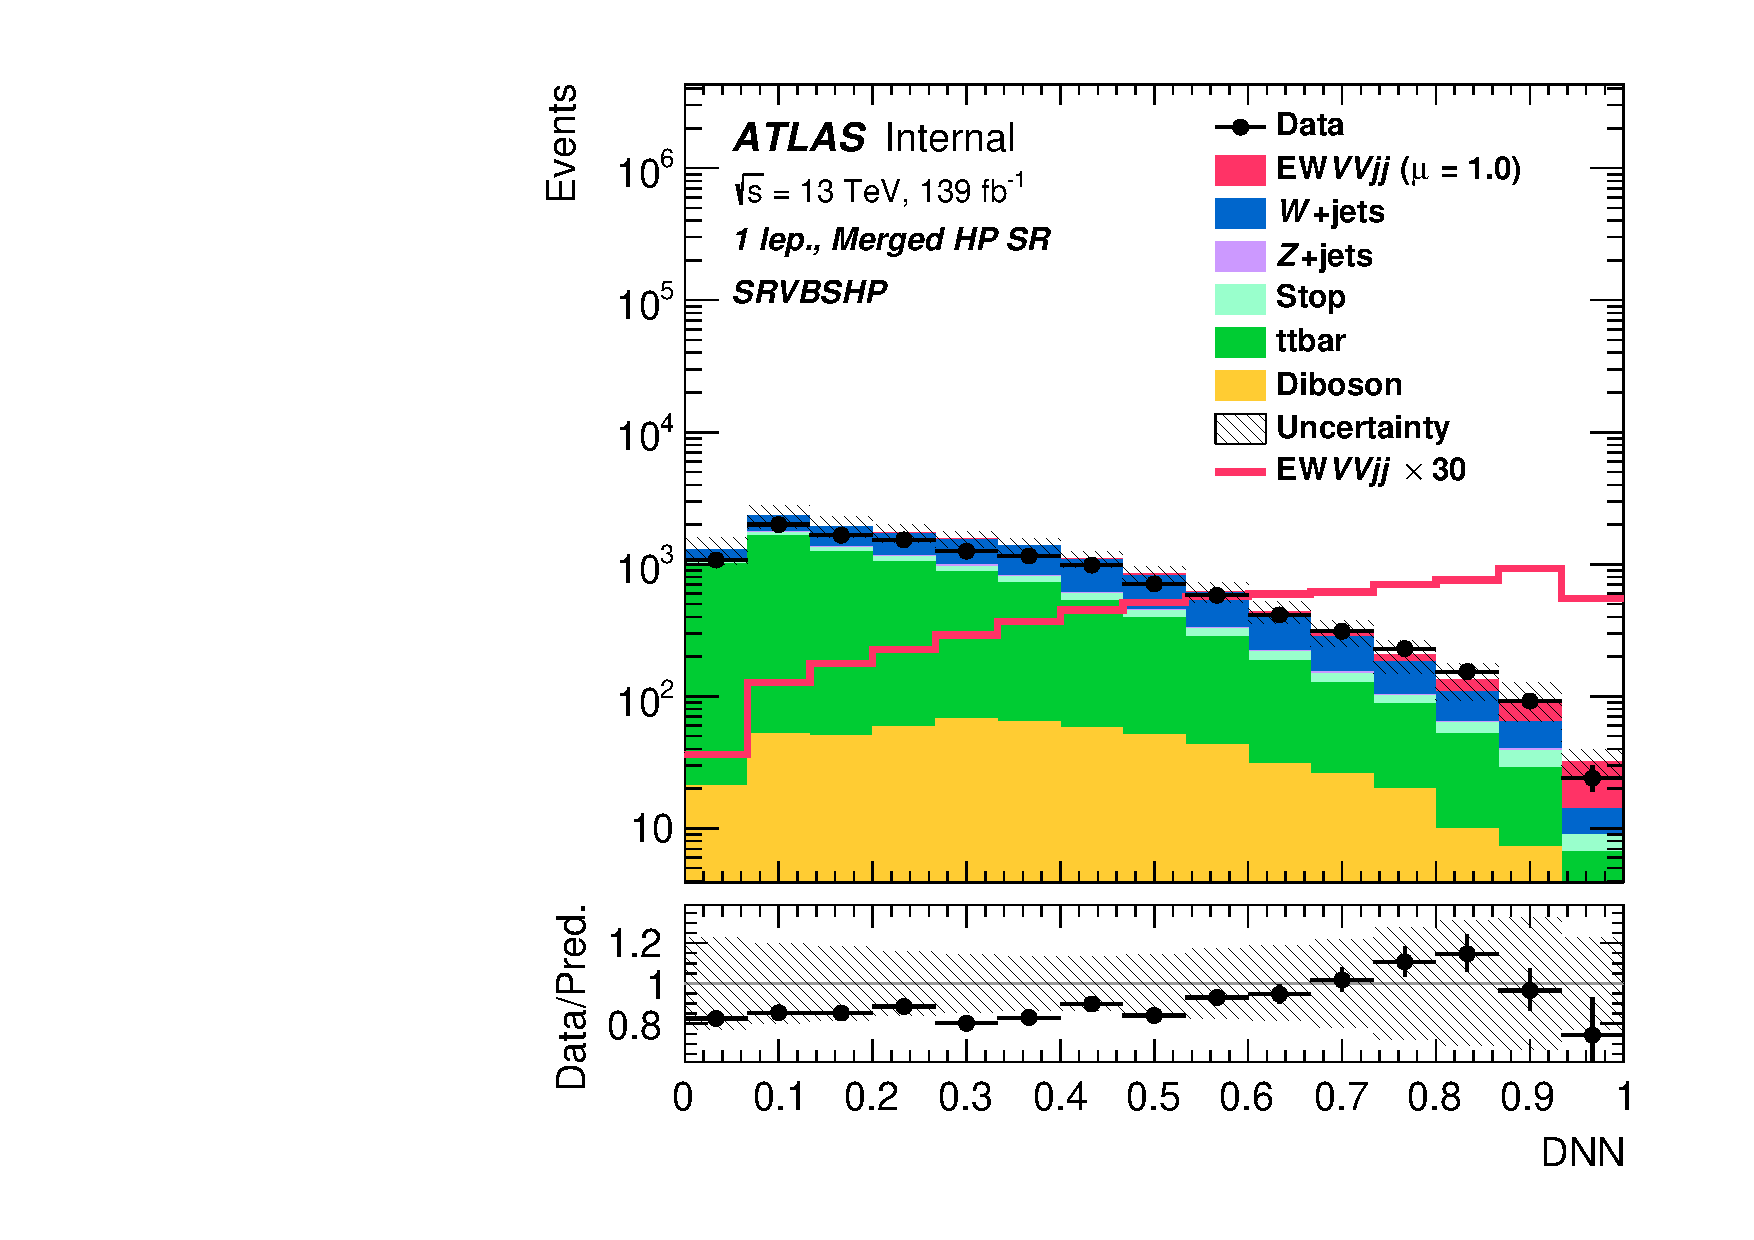
\includegraphics[width=\textwidth]{figures/FitResults/prefit/Region_distDNN_DSRVBSHP_BMin0_J0_incJet1_L1_T0_incFat1_Y6051_incTag1_Fat1_Prefitlog.pdf}
        \caption{Merged HP SR}
    \end{subfigure}
    \begin{subfigure}[b]{0.32\textwidth}
        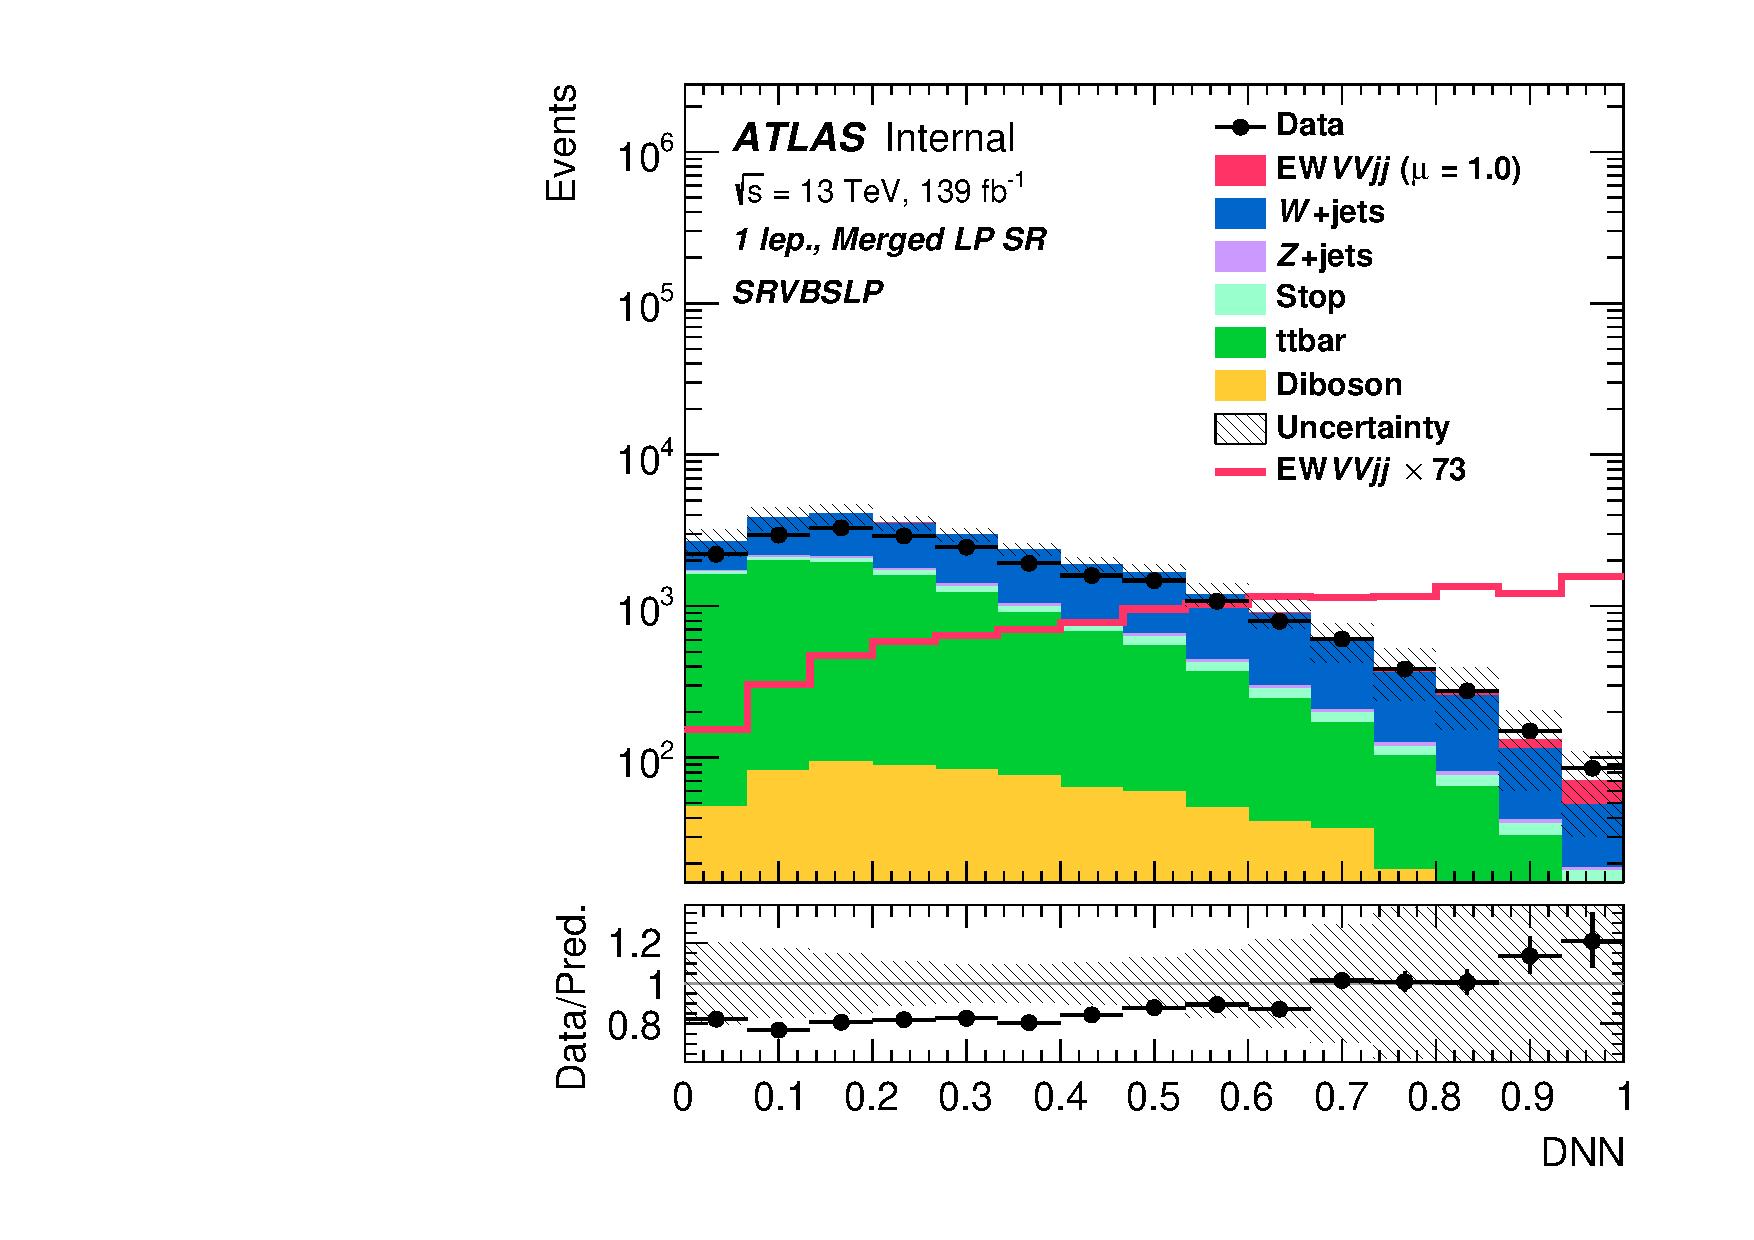
\includegraphics[width=\textwidth]{figures/FitResults/prefit/Region_distDNN_DSRVBSLP_BMin0_J0_incJet1_L1_T0_incFat1_Y6051_incTag1_Fat1_Prefitlog.pdf}
        \caption{Merged LP SR}
    \end{subfigure}
    \begin{subfigure}[b]{0.32\textwidth}
        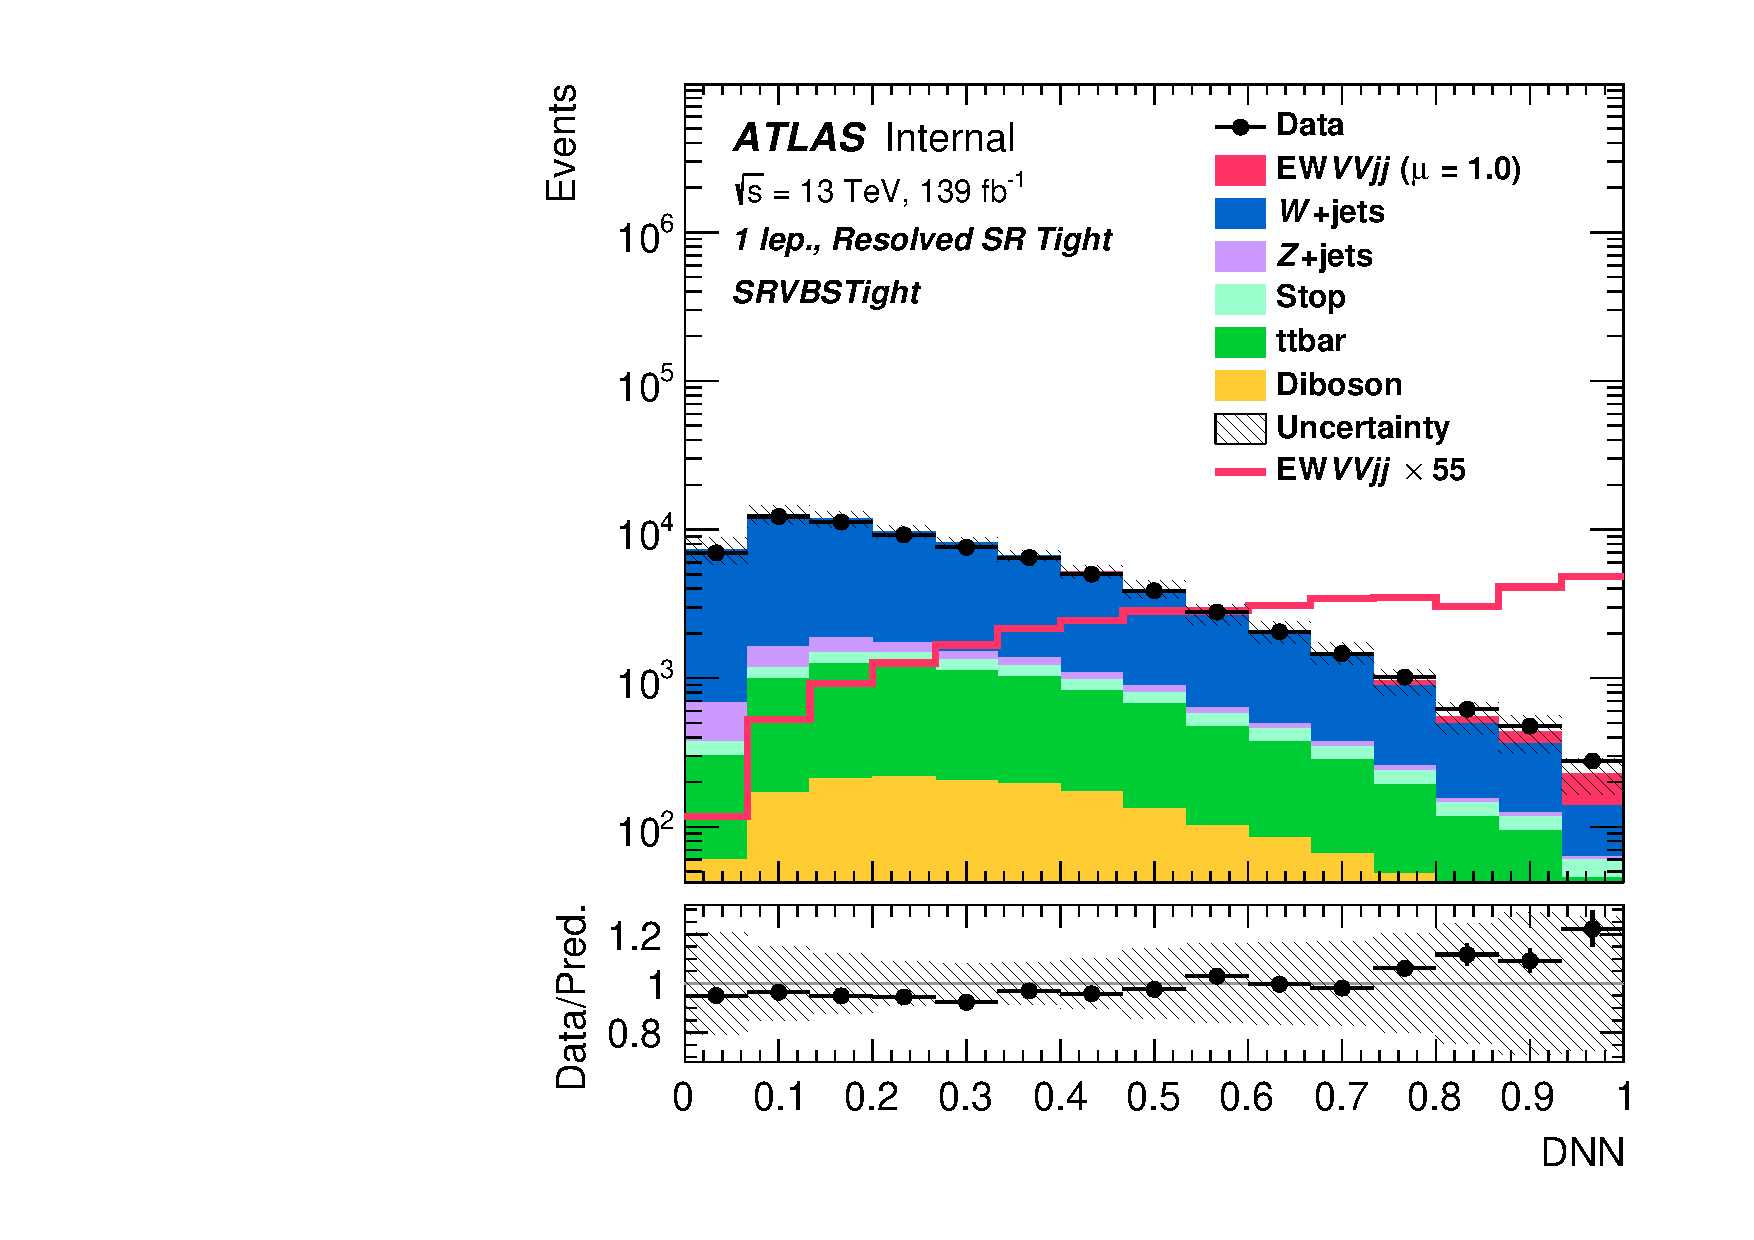
\includegraphics[width=\textwidth]{figures/FitResults/prefit/Region_distDNN_DSRVBSTight_BMin0_T0_Y6051_incTag1_J2_L1_incJet1_Prefitlog.pdf}
        \caption{Resolved SR}
    \end{subfigure}
    \\
    \begin{subfigure}[b]{0.32\textwidth}
        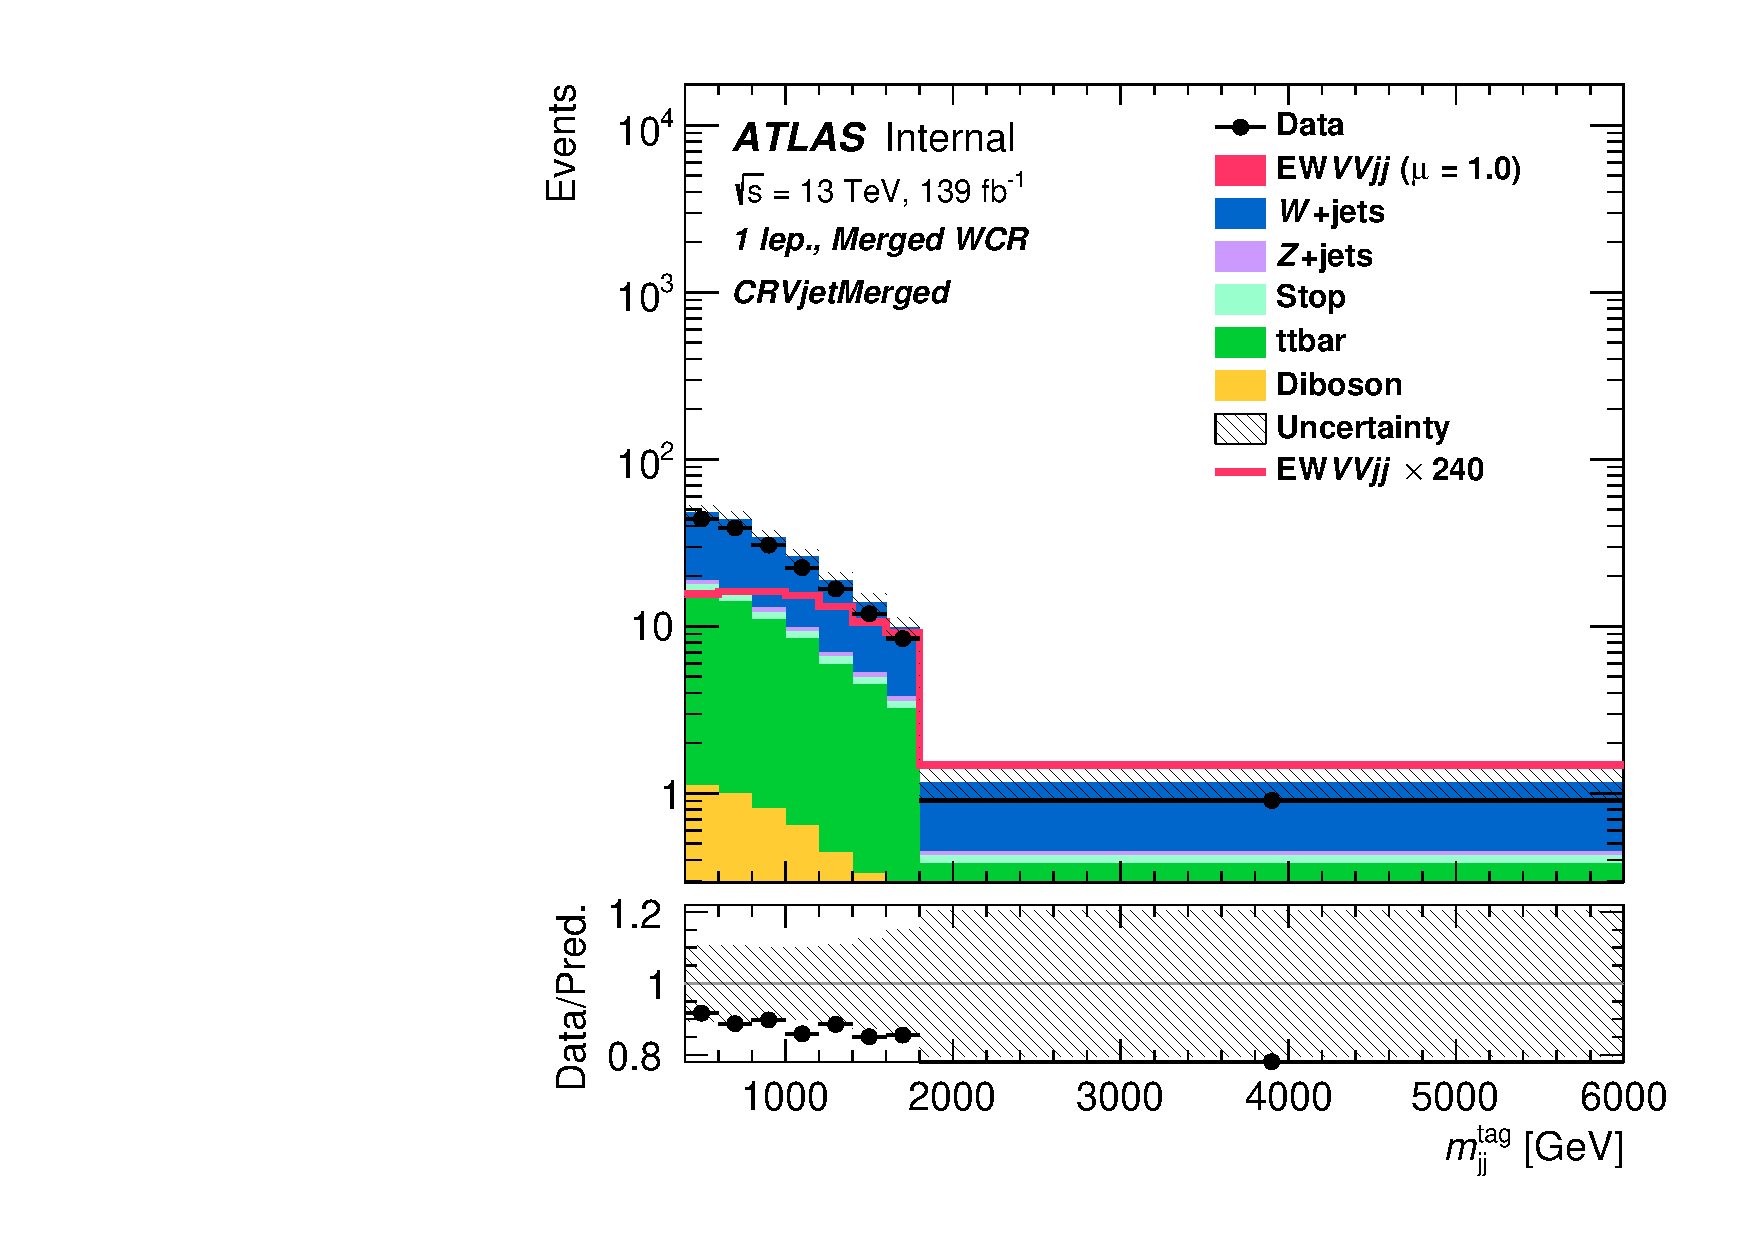
\includegraphics[width=\textwidth]{figures/FitResults/prefit/Region_disttagMjj_DCRVjetMerged_BMin0_J0_incJet1_L1_T0_incFat1_Y6051_incTag1_Fat1_Prefitlog.pdf}
        \caption{Merged WCR}
    \end{subfigure}
    \begin{subfigure}[b]{0.32\textwidth}
        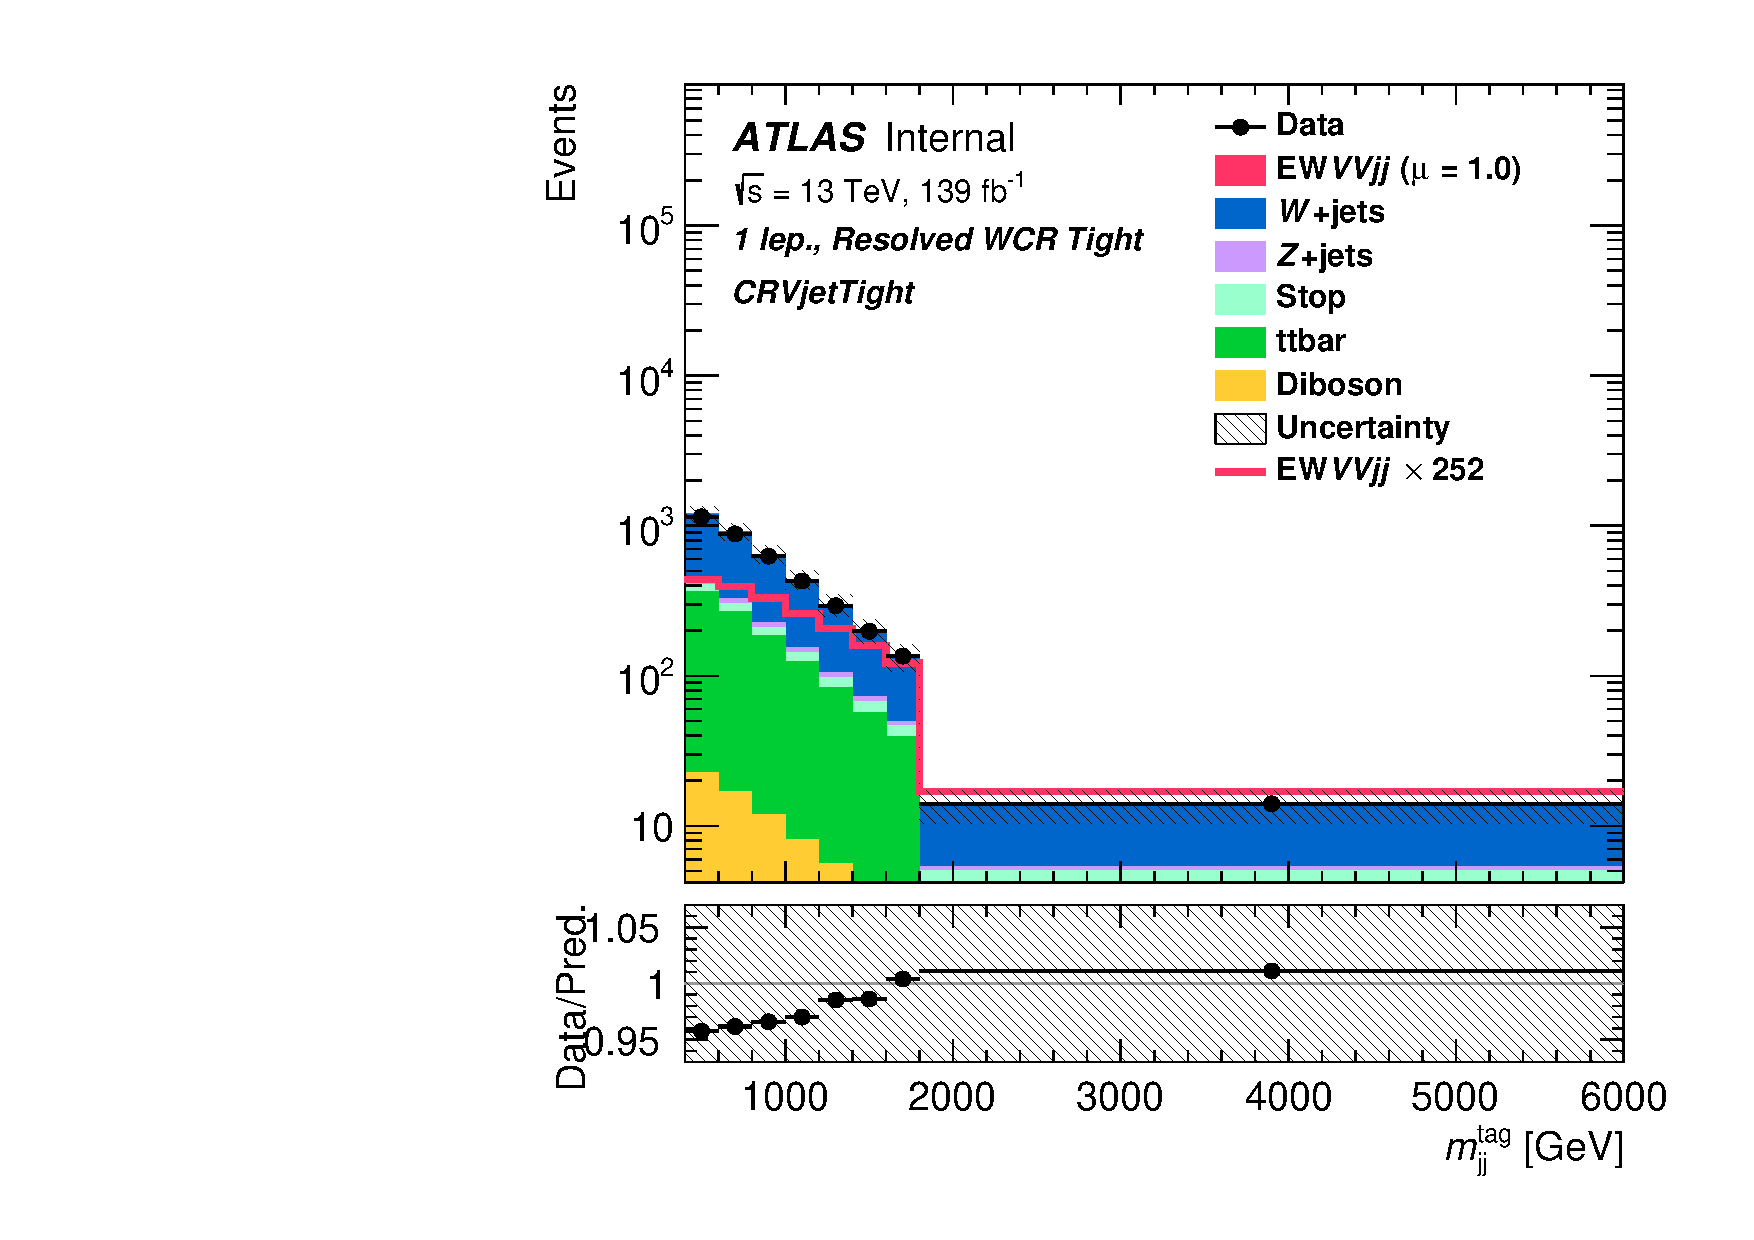
\includegraphics[width=\textwidth]{figures/FitResults/prefit/Region_disttagMjj_DCRVjetTight_BMin0_T0_Y6051_incTag1_J2_L1_incJet1_Prefitlog.pdf}
        \caption{Resolved WCR}
    \end{subfigure}
    \\
    \begin{subfigure}[b]{0.32\textwidth}
        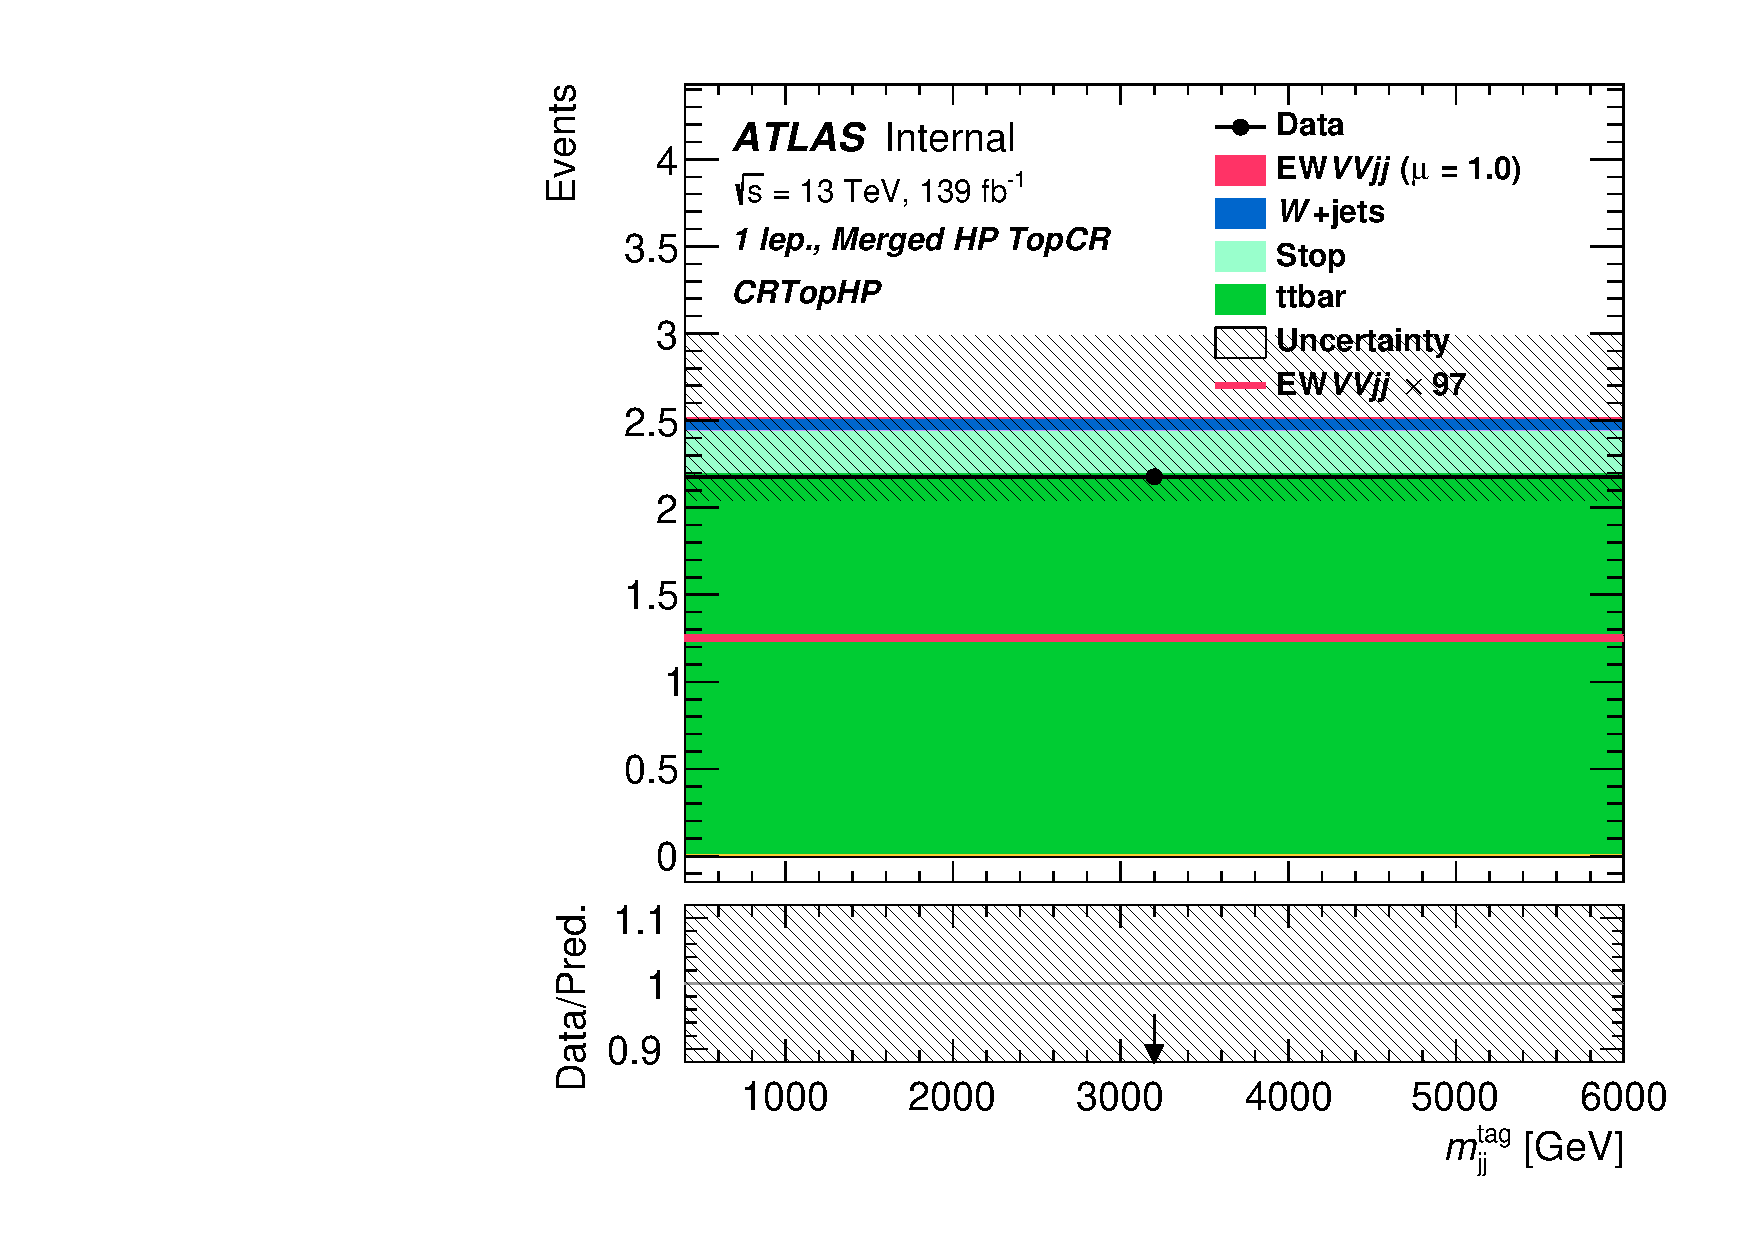
\includegraphics[width=\textwidth]{figures/FitResults/prefit/Region_disttagMjj_DCRTopHP_BMin0_J0_incJet1_L1_T0_incFat1_Y6051_incTag1_Fat1_Prefit.pdf}
        \caption{Merged HP TopCR}
    \end{subfigure}
    \begin{subfigure}[b]{0.32\textwidth}
        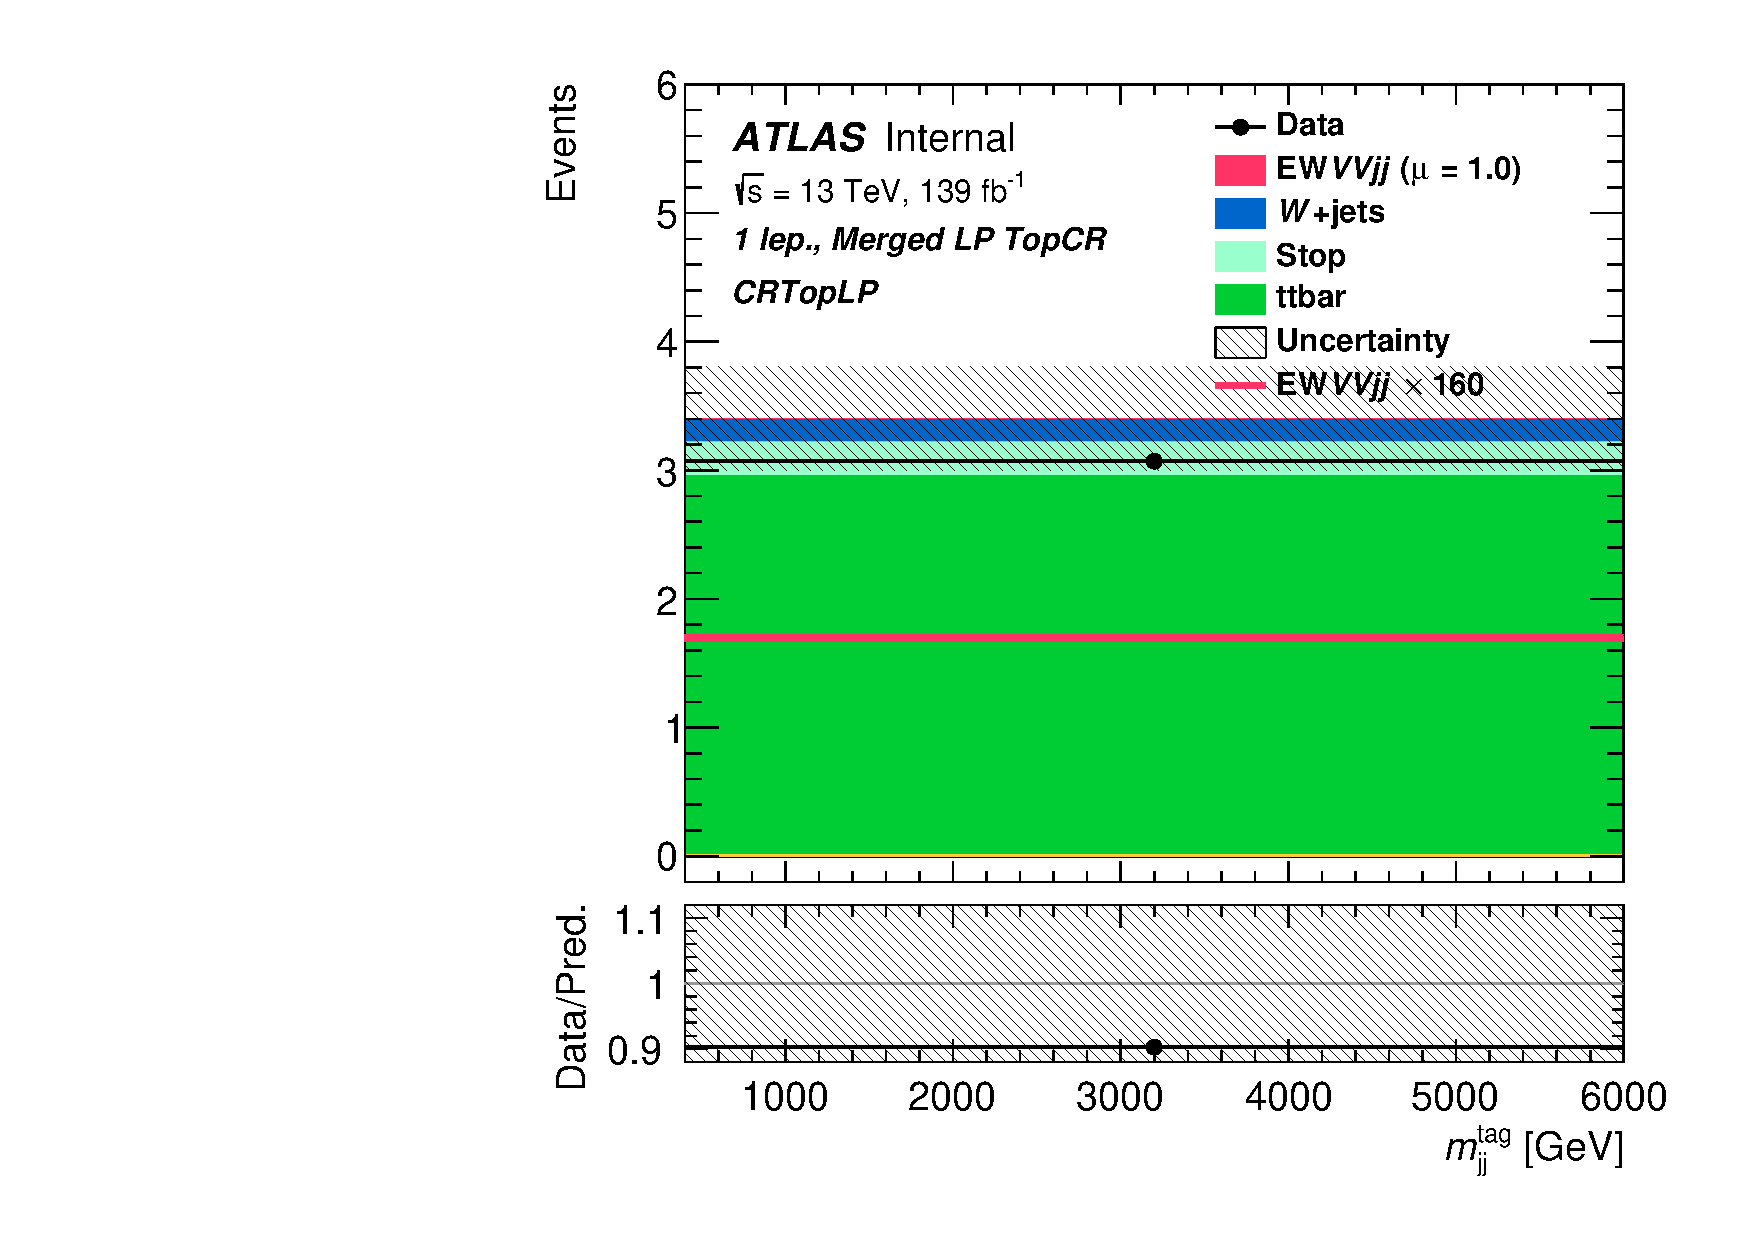
\includegraphics[width=\textwidth]{figures/FitResults/prefit/Region_disttagMjj_DCRTopLP_BMin0_J0_incJet1_L1_T0_incFat1_Y6051_incTag1_Fat1_Prefit.pdf}
        \caption{Merged LP TopCR}
    \end{subfigure}
    \begin{subfigure}[b]{0.32\textwidth}
        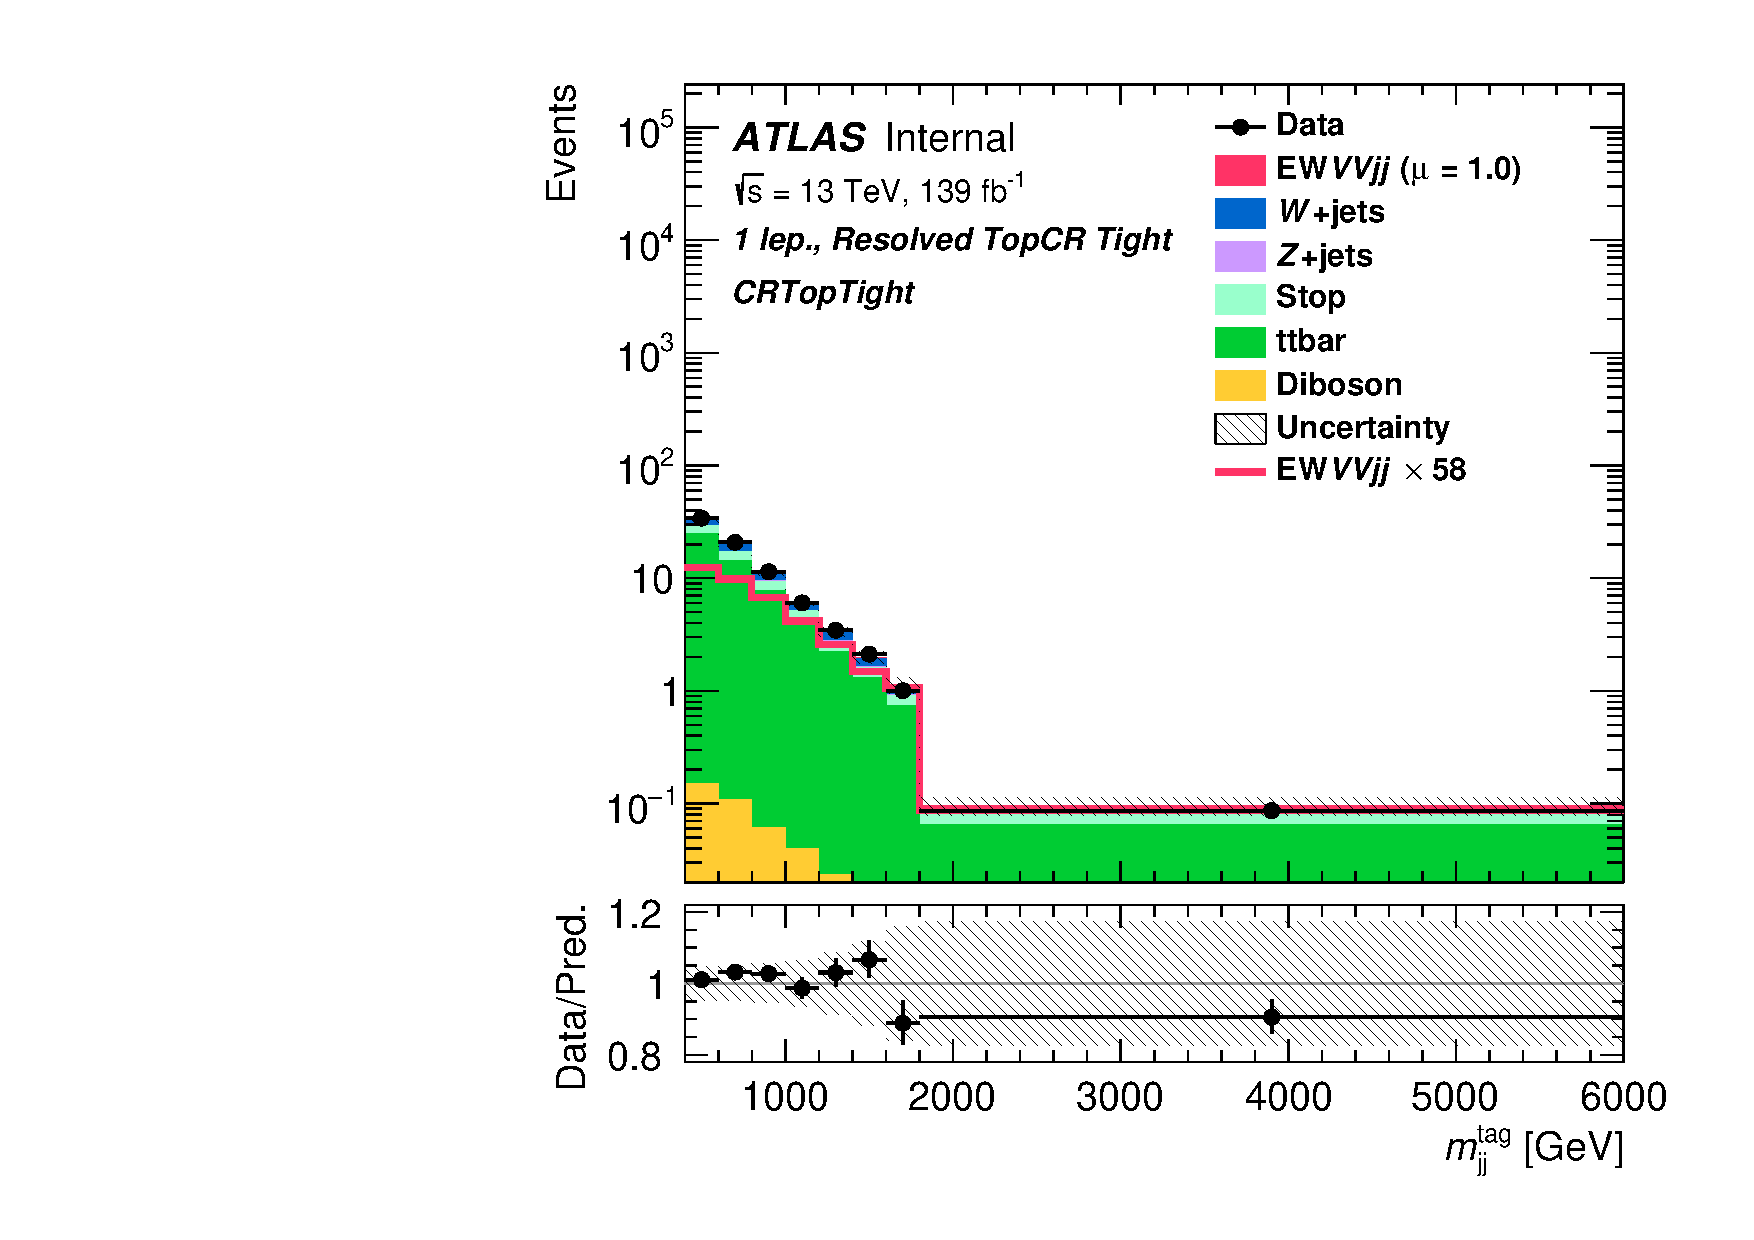
\includegraphics[width=\textwidth]{figures/FitResults/prefit/Region_disttagMjj_DCRTopTight_BMin0_T0_Y6051_incTag1_J2_L1_incJet1_Prefitlog.pdf}
        \caption{Resolved TopCR}
    \end{subfigure}
    \caption{Prefit plots for the 1 lepton channel. Data has been unblinded}
    \label{fig:fit_1lep_prefit}
\end{figure}


% \newcolumntype{d}{D{+}{\hspace{-3pt}\;\pm\;}{-1}}
%%%\documentclass{article}
%%%\usepackage{graphicx}
%%%\newcommand{\GeV}{\mathrm{GeV}}
%%%\newcommand{\ptv}{p_T^V}
%%%\begin{document}
\begin{table}
\centering
\small
\begin{tabular}{|l|c|}
\hline
\multicolumn{2}{|c|}{DNN\_SRVBSHP} \\ \hline
W & 4656.33 $\pm$ 599.26\\
Z & 155.86 $\pm$ 29.63\\
Diboson & 564.00 $\pm$ 208.79\\
stop & 720.09 $\pm$ 249.77\\
ttbar & 7724.82 $\pm$ 1531.65\\
\hline
Bkg & 13821.09 $\pm$ 2012.72\\
\hline
EW6lvqq & 228.59 $\pm$ 41.37\\
\hline
Signal & 228.59 $\pm$ 41.37\\
SignalExpected & 228.59 $\pm$ 41.37\\
\hline
S/B & 1.65e-02\\
S/sqrt(S+B) & 1.93e+00\\
\hline
data & 12178\\ \hline
\end{tabular}
%%%\end{table}
%%%
%%%
%%%\begin{table}
%%%\centering
%%%\small
\begin{tabular}{|l|c|}
\hline
 \multicolumn{2}{|c|}{DNN\_SRVBSLP}\\ \hline
W & 13507.48 $\pm$ 1306.67\\
Z & 433.51 $\pm$ 75.10\\
Diboson & 759.72 $\pm$ 276.17\\
stop & 974.63 $\pm$ 316.11\\
ttbar & 10758.23 $\pm$ 1251.68\\
\hline
Bkg & 26433.56 $\pm$ 2560.55\\
\hline
EW6lvqq & 180.21 $\pm$ 37.21\\
\hline
Signal & 180.21 $\pm$ 37.21\\
SignalExpected & 180.21 $\pm$ 37.21\\
\hline
S/B & 6.82e-03\\
S/sqrt(S+B) & 1.10e+00\\
\hline
data & 22158\\ \hline
\end{tabular}
%%%\end{table}
%%%
%%%
%%%\begin{table}
%%%\centering
%%%\small
\begin{tabular}{|l|c|}
\hline
 \multicolumn{2}{|c|}{DNN\_SRVBSRes}\\ \hline
W & 60551.72 $\pm$ 5916.55\\
Z & 2114.42 $\pm$ 425.26\\
Diboson & 1723.35 $\pm$ 582.92\\
stop & 1750.76 $\pm$ 541.16\\
ttbar & 7330.60 $\pm$ 299.18\\
\hline
Bkg & 73470.84 $\pm$ 6611.96\\
\hline
EW6lvqq & 662.01 $\pm$ 56.52\\
\hline
Signal & 662.01 $\pm$ 56.52\\
SignalExpected & 662.01 $\pm$ 56.52\\
\hline
S/B & 9.01e-03\\
S/sqrt(S+B) & 2.43e+00\\
\hline
data & 71272\\ \hline
\end{tabular}
\caption{Prefit event yields for the analysis SRs in the 1 lepton channel.}
\label{tab:1lepPrefitYield_SR}
\end{table}


\begin{table}
\centering
\small
\begin{tabular}{|l|c|}
\hline
 \multicolumn{2}{|c|}{tagMjj\_CRTopHP}\\ \hline
W & 352.82 $\pm$ 43.34\\
Z & 16.22 $\pm$ 3.13\\
Diboson & 41.79 $\pm$ 15.53\\
stop & 1342.33 $\pm$ 456.84\\
ttbar & 12267.00 $\pm$ 2374.62\\
\hline
Bkg & 14020.16 $\pm$ 2635.77\\
\hline
EW6lvqq & 72.15 $\pm$ 13.03\\
\hline
Signal & 72.15 $\pm$ 13.03\\
SignalExpected & 72.15 $\pm$ 13.03\\
\hline
S/B & 5.15e-03\\
S/sqrt(S+B) & 6.08e-01\\
\hline
data & 12195\\ \hline
\end{tabular}
%%%\end{table}
%%%
%%%
%%%\begin{table}
%%%\centering
%%%\small
\begin{tabular}{|l|c|}
\hline
 \multicolumn{2}{|c|}{tagMjj\_CRTopLP}\\ \hline
W & 949.62 $\pm$ 77.62\\
Z & 43.10 $\pm$ 7.66\\
Diboson & 65.63 $\pm$ 22.52\\
stop & 1426.00 $\pm$ 466.82\\
ttbar & 16508.02 $\pm$ 1970.36\\
\hline
Bkg & 18992.37 $\pm$ 2239.62\\
\hline
EW6lvqq & 59.17 $\pm$ 9.99\\
\hline
Signal & 59.17 $\pm$ 9.99\\
SignalExpected & 59.17 $\pm$ 9.99\\
\hline
S/B & 3.12e-03\\
S/sqrt(S+B) & 4.29e-01\\
\hline
data & 17195\\ \hline
\end{tabular}
%%%\end{table}
%%%
%%%
%%%\clearpage
%%%
%%%
%%%\begin{table}
%%%\centering
%%%\small
\begin{tabular}{|l|c|}
\hline
 \multicolumn{2}{|c|}{tagMjj\_CRTopRes}\\ \hline
W & 2092.27 $\pm$ 102.60\\
Z & 96.04 $\pm$ 18.42\\
Diboson & 84.24 $\pm$ 28.43\\
stop & 2132.59 $\pm$ 646.43\\
ttbar & 11368.00 $\pm$ 303.73\\
\hline
Bkg & 15773.14 $\pm$ 776.66\\
\hline
EW6lvqq & 138.07 $\pm$ 6.64\\
\hline
Signal & 138.07 $\pm$ 6.64\\
SignalExpected & 138.07 $\pm$ 6.64\\
\hline
S/B & 8.75e-03\\
S/sqrt(S+B) & 1.09e+00\\
\hline
data & 16137\\ \hline
\end{tabular}
%%%\end{table}
%%%
%%%
%%%\begin{table}
%%%\centering
%%%\small
\begin{tabular}{|l|c|}
\hline
 \multicolumn{2}{|c|}{tagMjj\_CRWjetMerged}\\ \hline
W & 27122.54 $\pm$ 3139.15\\
Z & 937.92 $\pm$ 172.50\\
Diboson & 1050.98 $\pm$ 363.58\\
stop & 1407.69 $\pm$ 442.73\\
ttbar & 13290.86 $\pm$ 1368.18\\
\hline
Bkg & 43809.98 $\pm$ 4299.96\\
\hline
EW6lvqq & 106.15 $\pm$ 11.62\\
\hline
Signal & 106.15 $\pm$ 11.62\\
SignalExpected & 106.15 $\pm$ 11.62\\
\hline
S/B & 2.42e-03\\
S/sqrt(S+B) & 5.07e-01\\
\hline
data & 38486\\ \hline
\end{tabular}
%%%\end{table}
%%%
%%%
%%%\begin{table}
%%%\centering
%%%\small
\begin{tabular}{|l|c|}
\hline
 \multicolumn{2}{|c|}{tagMjj\_CRWjetRes}\\ \hline
W & 527592.75 $\pm$ 83268.24\\
Z & 20700.18 $\pm$ 6182.92\\
Diboson & 15641.74 $\pm$ 5369.28\\
stop & 33952.01 $\pm$ 10877.37\\
ttbar & 226711.24 $\pm$ 18682.68\\
\hline
Bkg & 824597.92 $\pm$ 112159.27\\
\hline
EW6lvqq & 1790.20 $\pm$ 151.38\\
\hline
Signal & 1790.20 $\pm$ 151.38\\
SignalExpected & 1790.20 $\pm$ 151.38\\
\hline
S/B & 2.17e-03\\
S/sqrt(S+B) & 1.97e+00\\
\hline
data & 801406\\ \hline
\end{tabular}
\caption{Prefit event yields for the analysis CRs in the 1 lepton channel.}
\label{tab:1lepPrefitYield_CR}
\end{table}


%%\end{document}


%%%%

\clearpage
\subsection{Asimov Fit Results}

A fit to the full SRs using Asimov data is performed to identify constraints within the fit model. 
Figures~\ref{fig:fit_1lep_fcc_asimov}, \ref{fig:fit_1lep_corr_all}, and \ref{fig:fit_1lep_ranking_all} show the pulls, correlations, and rankings, respectively, of the NPs used in the fit.

In the context of the pull plot, the black boxes represent an approximate measure of how well the fitted pull aligns with the postfit constraint for a given NP. A smaller pull that appears less constrained is generally less significant than a larger pull with a tight constraint. This concept is further elaborated in the reference~\cite{morange:tel-03341303}, which provides detailed insights into the statistical interpretation of these pulls and constraints in the analysis.

A brief commentary on the identified relevant constraints is provided below:

\begin{itemize}

\item \texttt{SysMJJREWEIGHT\_100per\_W+jets} (L1\_Fat1 for merged and L1\_J2 for resolved) 
represents uncertainties related to the reweighting of \mjjtag in both merged and resolved regions. These constraints are expected due to the application of 100\% uncertainties to the \mjjtag reweighting, allowing the control regions to effectively constrain these systematic uncertainties (see Section~\ref{subsec:bkg_uncer_mjjrew}).

\item \texttt{SysMODEL\_Wjets\_MadGraph} 
arises from the shape differences between the Sherpa and MadGraph samples. This uncertainty is significant in our analysis due to the known modeling disparities between these two generators, especially in regions of high \mjjtag and jet multiplicity. The influence of this uncertainty on the signal strength $\mu$ is notable, approximately $8\%$ in the resolved regime and somewhat lesser in the merged regime, as depicted in the ranking plot (Figure~\ref{fig:fit_1lep_ranking_all}).

\item \texttt{SysMODEL\_ttbar\_PwHwg7} 
uncertainties refer to the modeling uncertainties associated with the \ttbar background, which are derived from alternative sample comparisons. The analysis relies on the constraints obtained from the dedicated TCRs to mitigate these uncertainties.

\item \texttt{SysPRW\_DATASF} and \texttt{SysJET\_Pileup\_Offset} 
uncertainties are related to pile-up effects. These systematic uncertainties significantly influence the shapes of forward jets and jet track multiplicity (quark-gluon tagging variables). This effect is detailed in Section~\ref{subsec:bkg_uncer_qg}.

\item \texttt{SysTheoryQCD\_W} 
represents the QCD theory scale uncertainty impacting the \Wjets prediction. This uncertainty is effectively constrained by the shape of the final discriminant (DNN) in the resolved signal region, as illustrated in Figure~\ref{fig:PDFUnc1Lep_QCD}.

\item \texttt{SysTheoryISR\_ttbar} and \texttt{SysTheoryFSR\_Top} 
represent theory uncertainties in \ttbar production with additional radiation in the initial or final states, as detailed in Section~\ref{subsec:isr_fsr_unc}. There is a top modeling issue in the merged control regions. Given that these nuisance parameters do not directly impact the signal, we simplify our analysis by employing a single bin for the merged TCRs.

\item \texttt{SysFATJET\_BJT\_JET\_JetTagSF\_Hadronisation} represents the uncertainty associated with the hadronisation modeling.

\end{itemize}


\begin{figure}[ht]
      \centering
        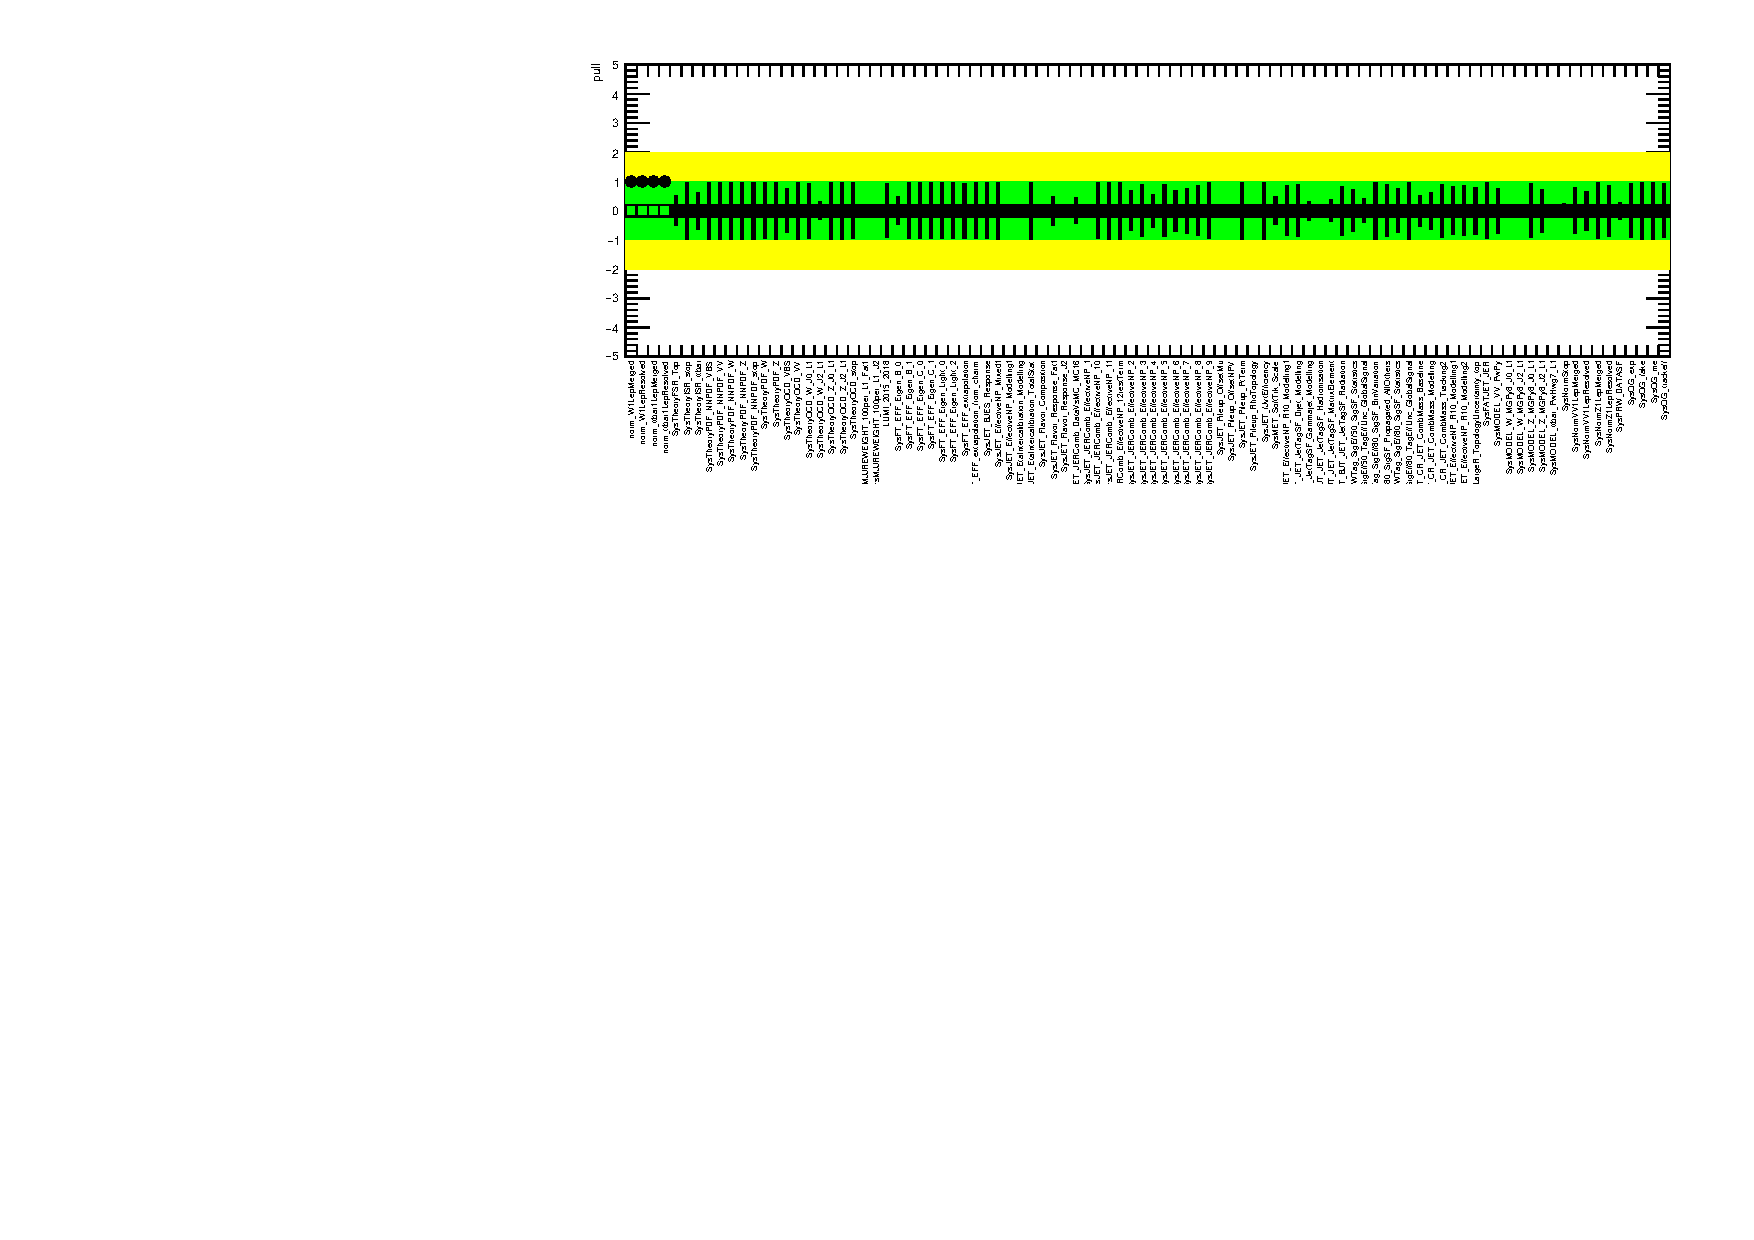
\includegraphics[width=\linewidth]{figures/Fit_fcc/AsimovFit/NP_allExceptGammas.pdf}
        \caption{Fit cross-check, conditional fit ($\mu=1$) to asimov data for the 1 lepton channel.}
       \label{fig:fit_1lep_fcc_asimov}
\end{figure}

\begin{figure}[ht]
      \centering
        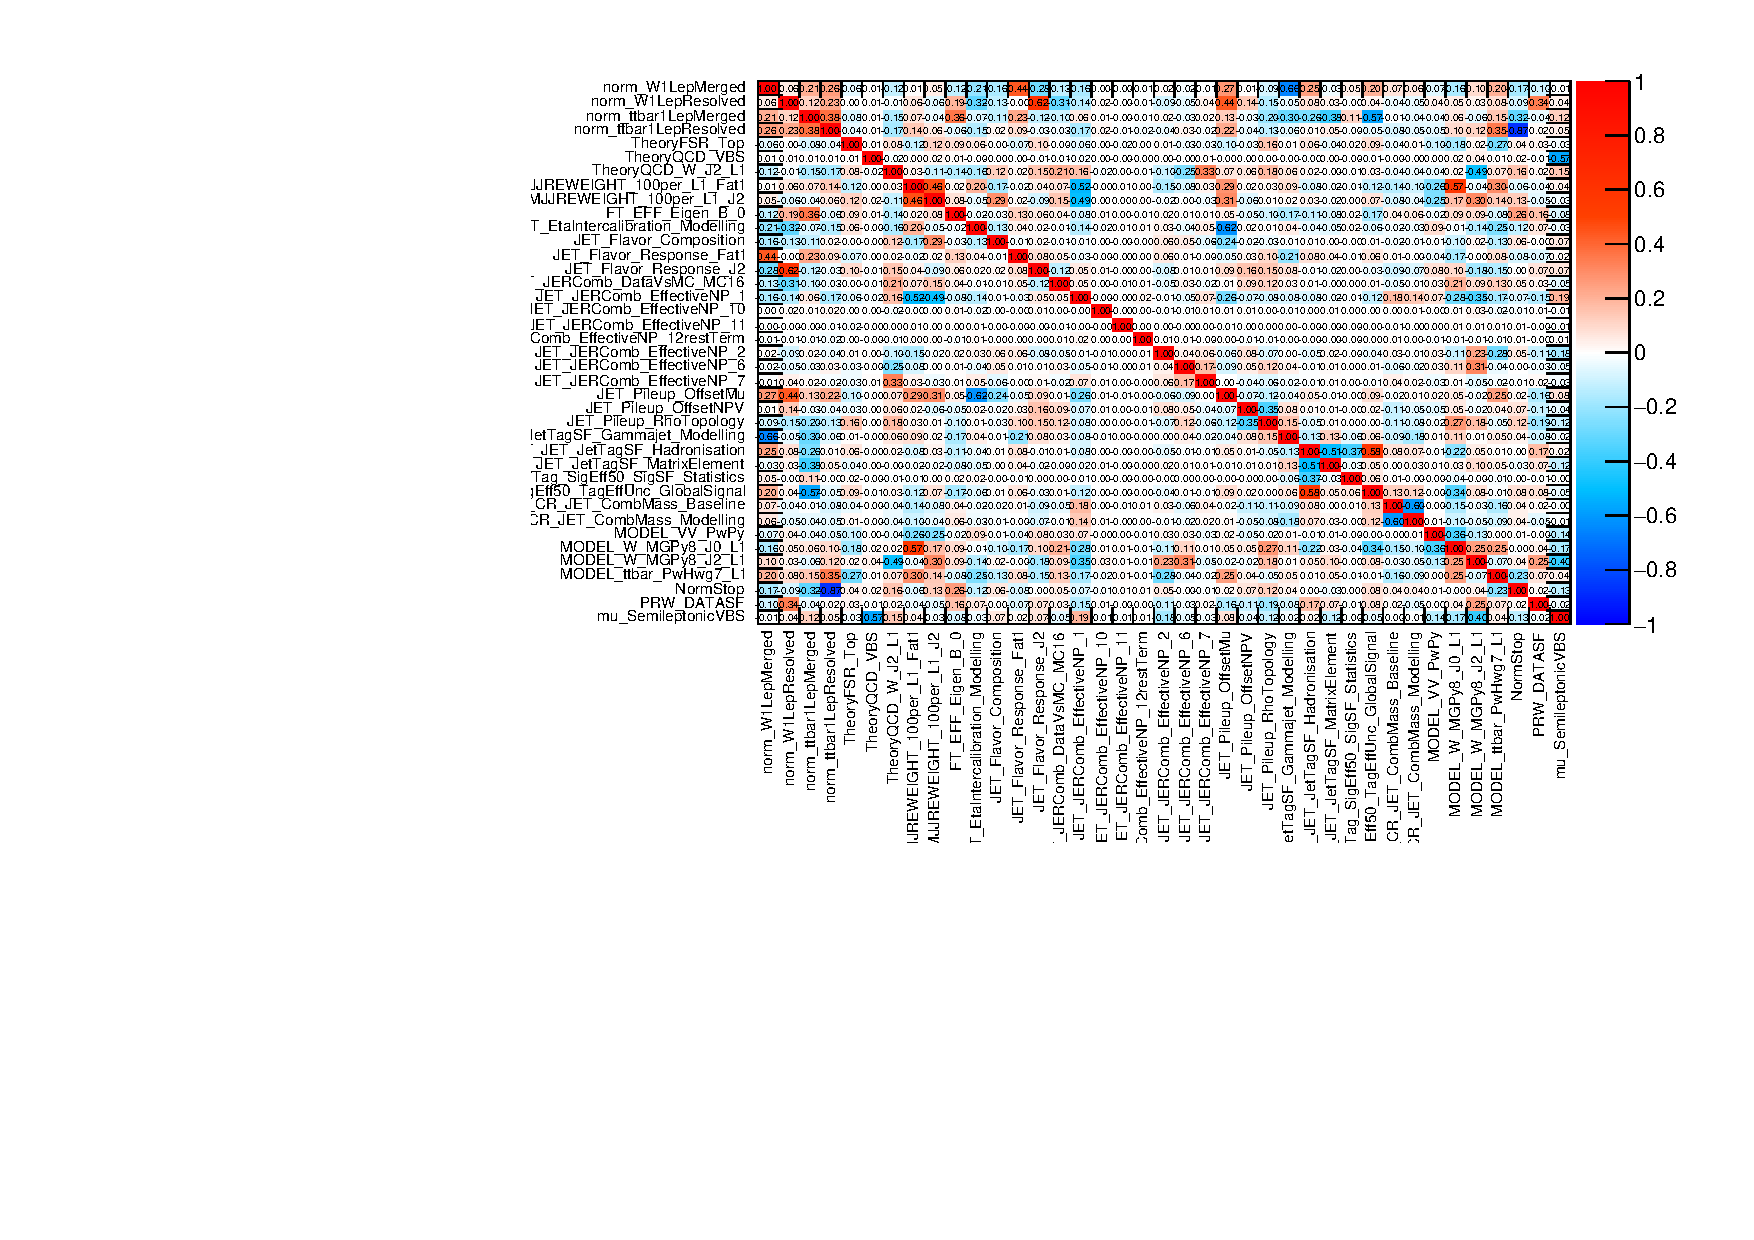
\includegraphics[width=\linewidth]{figures/Fit_fcc/AsimovFit_uncon/corr_HighCorrNoMCStat.pdf}
        \caption{Correlations for unconditional fit ($\mu=1$) to asimov data in the full range, for the 1 lepton channel.}
       \label{fig:fit_1lep_corr_all}
\end{figure}

\begin{figure}[ht]
      \centering
        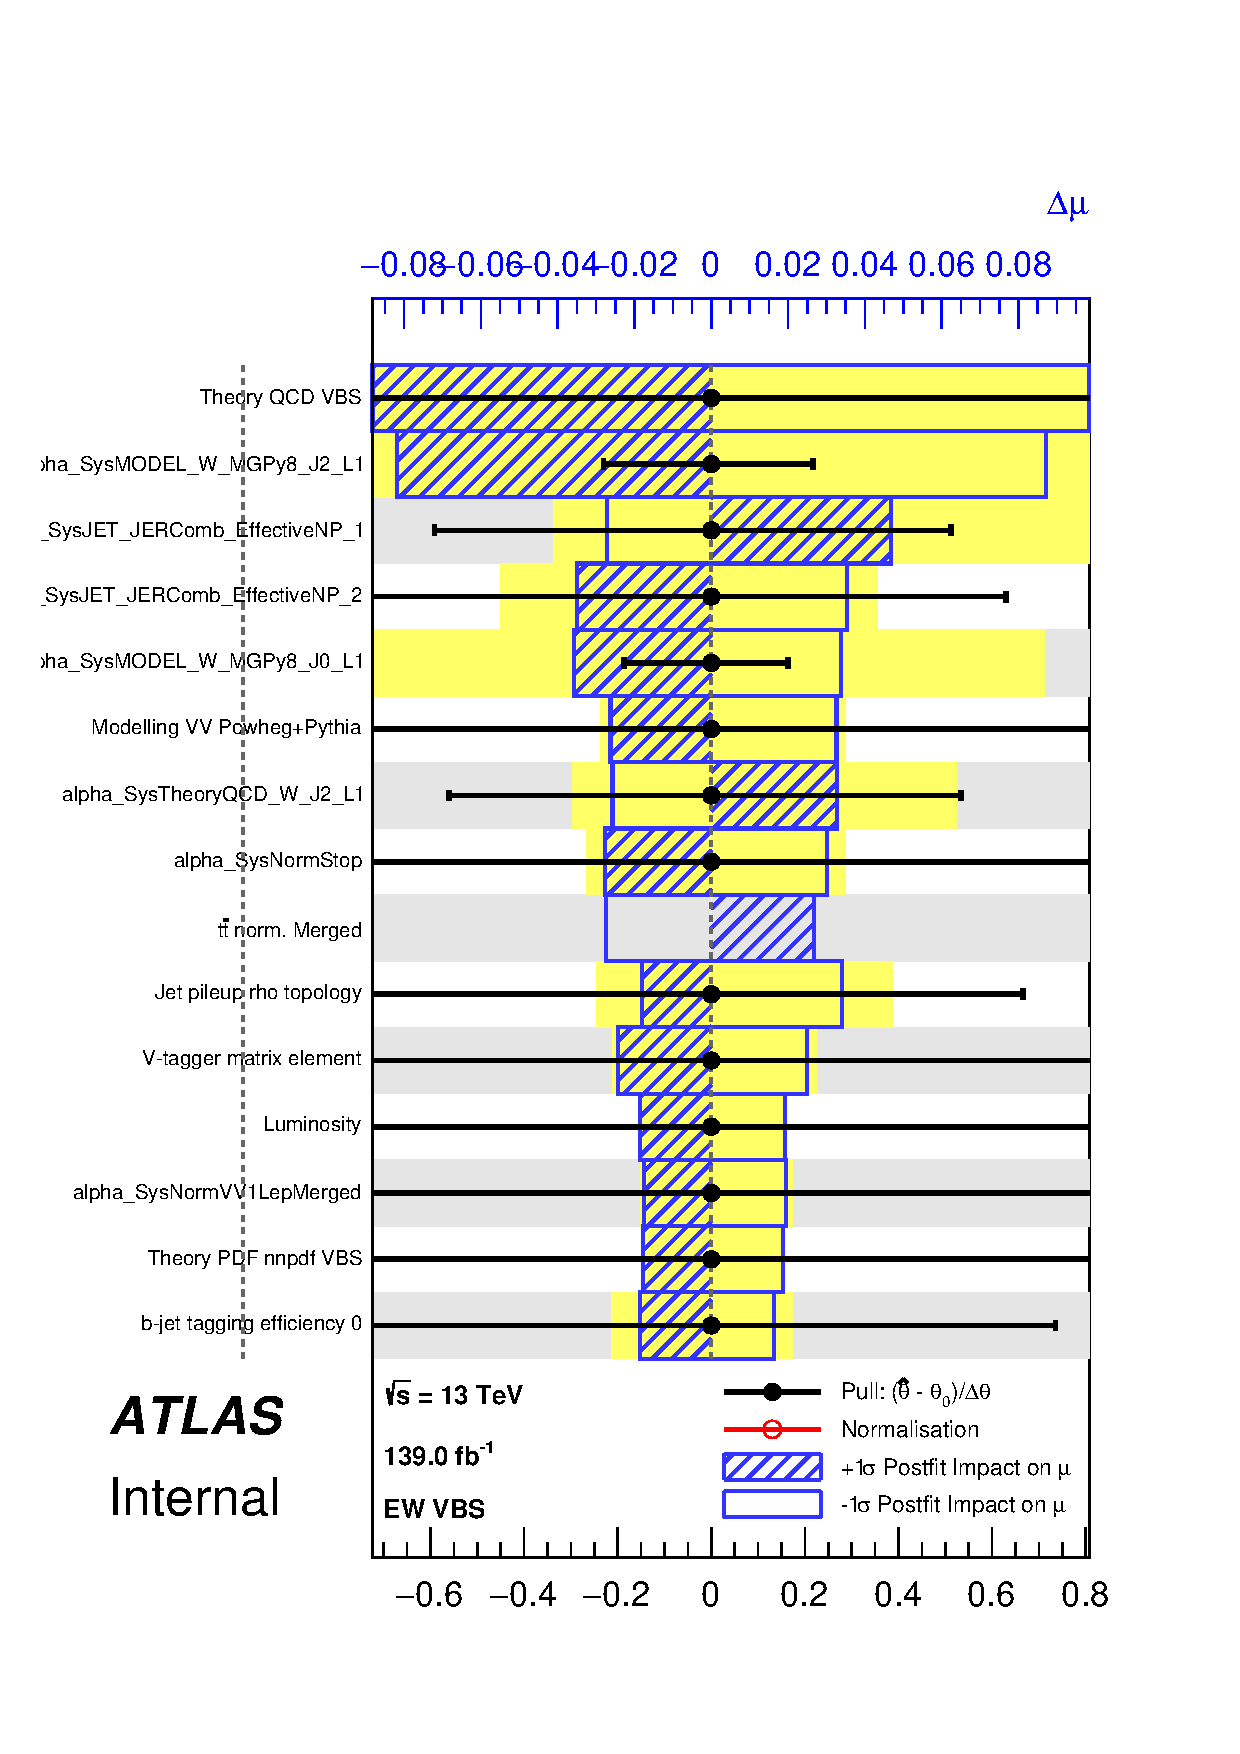
\includegraphics[width=0.5\textwidth]{figures/Fit_np_rank/pulls_mu_Asimov/pulls_mu_SemileptonicVBS_5.pdf}
        \caption{Ranking plot for unconditional fit ($\mu=1$) to asimov data in the full range, for the 1 lepton channel.}
       \label{fig:fit_1lep_ranking_all}
\end{figure}

~
  
%%%
%1-lep DNN ML
\clearpage
\section{Fit Results with Unblinded Data}

%%%Using fitting methodology aligned with the procedures outlined in the previous sections in this chapter, we have seen some promising preliminary results with the DNN.
%%%Table \ref{tab:significance_1lepdnn} shows the expected and observed significances for the \olep channel. The observed significance exceeds the 5$\sigma$ threshold. Although uncertainties from Shower systematics are not accounted for in the DNN approach fitting, the results are robust enough to act as a corroborative crosscheck against the baseline analysis.
%%%
%%%The essential variables incorporated into the fit part of the study are the \mjjtag distribution and the final DNN score; a detailed enumeration of the regions and variables applied in the DNN approach's fit is presented in Table \ref{tab:fitregions_1lepdnn}.
%%%
%%%\begin{table}[htb!]
%%%  \centering
%%%  \begin{tabular}{lccc}
%%%          \toprule\midrule
%%%          \multirow{2}{*}{Regions} & \multicolumn{3}{c}{1lep channel fit model} \\
%%%          \cmidrule{2-4}
%%%                & Merged high-purity & Merged low-purity & Resolved \\
%%%          \midrule
%%%          SR     & DNN & DNN & DNN \\
%%%          WCR    & \multicolumn{2}{c}{\mjjtag} & \mjjtag \\
%%%          TopCR  & One bin & One bin & \mjjtag \\
%%%          \midrule
%%%          \bottomrule
%%%  \end{tabular}
%%%\caption{\label{tab:fitregions_1lepdnn} Summary of the regions from 1lep channel entering the likelihood of the fit models.
%%%``One bin'' implies that a single bin without any shape information is used in the corresponding fit region.}
%%%\end{table}

Using the methodology detailed in earlier sections of this chapter, we have obtained promising preliminary unblinded results using the DNN. 
Table \ref{tab:significance_1lepdnn} presents both expected and observed significances for the \olep channel. 
The expected significance is derived from Asimov data, incorporating adjustments for background normalization and nuisance parameters. 
Remarkably, the observed significance from actual data surpasses the critical 5$\sigma$ threshold, 
and this would be the first time we achieve this level of significance in the semileptonic final states for the electroweak $VV+jj$ production within a VBS-enhanced phase space.
We observe some deficit compared to the expected significance in the \olep channel.
Although the DNN approach fitting does not account for some signal uncertainties from EWK-QCD interference and shower systematics, the results are robust enough to serve as a corroborative cross-check against other baseline analyses using different ML approaches.

\begin{table}[h]
  \centering
  \begin{tabular}{|c|c|}
    \hline
           & 1-lep \\
    \hline
    Expected pre-fit significance & 5.39 \\
    \hline
    Expected post-fit significance & 5.98 \\
    \hline
    Observed significance & 5.78 \\
    \hline
  \end{tabular}
  \caption{Expected and observed significances for the \olep channel.}
  \label{tab:significance_1lepdnn}
\end{table}

Preliminary DNN(\olep) fit yields a signal strength parameter $\mu_{VBS} = 1.16 \pm 0.25$. 
Post-fit distributions for the 1-lep Signal Regions (SRs) with full range data are shown in Figure \ref{fig:postfitsr_1lepdnn}, while the corresponding distributions for the 1-lep Control Regions (CRs) are shown in Figure \ref{fig:postfitcr_1lepdnn}.
These distributions demonstrate a satisfactory agreement between the data and the MC simulations.

\begin{figure}[h]
  \centering
  \subfloat[Merged HP]{
    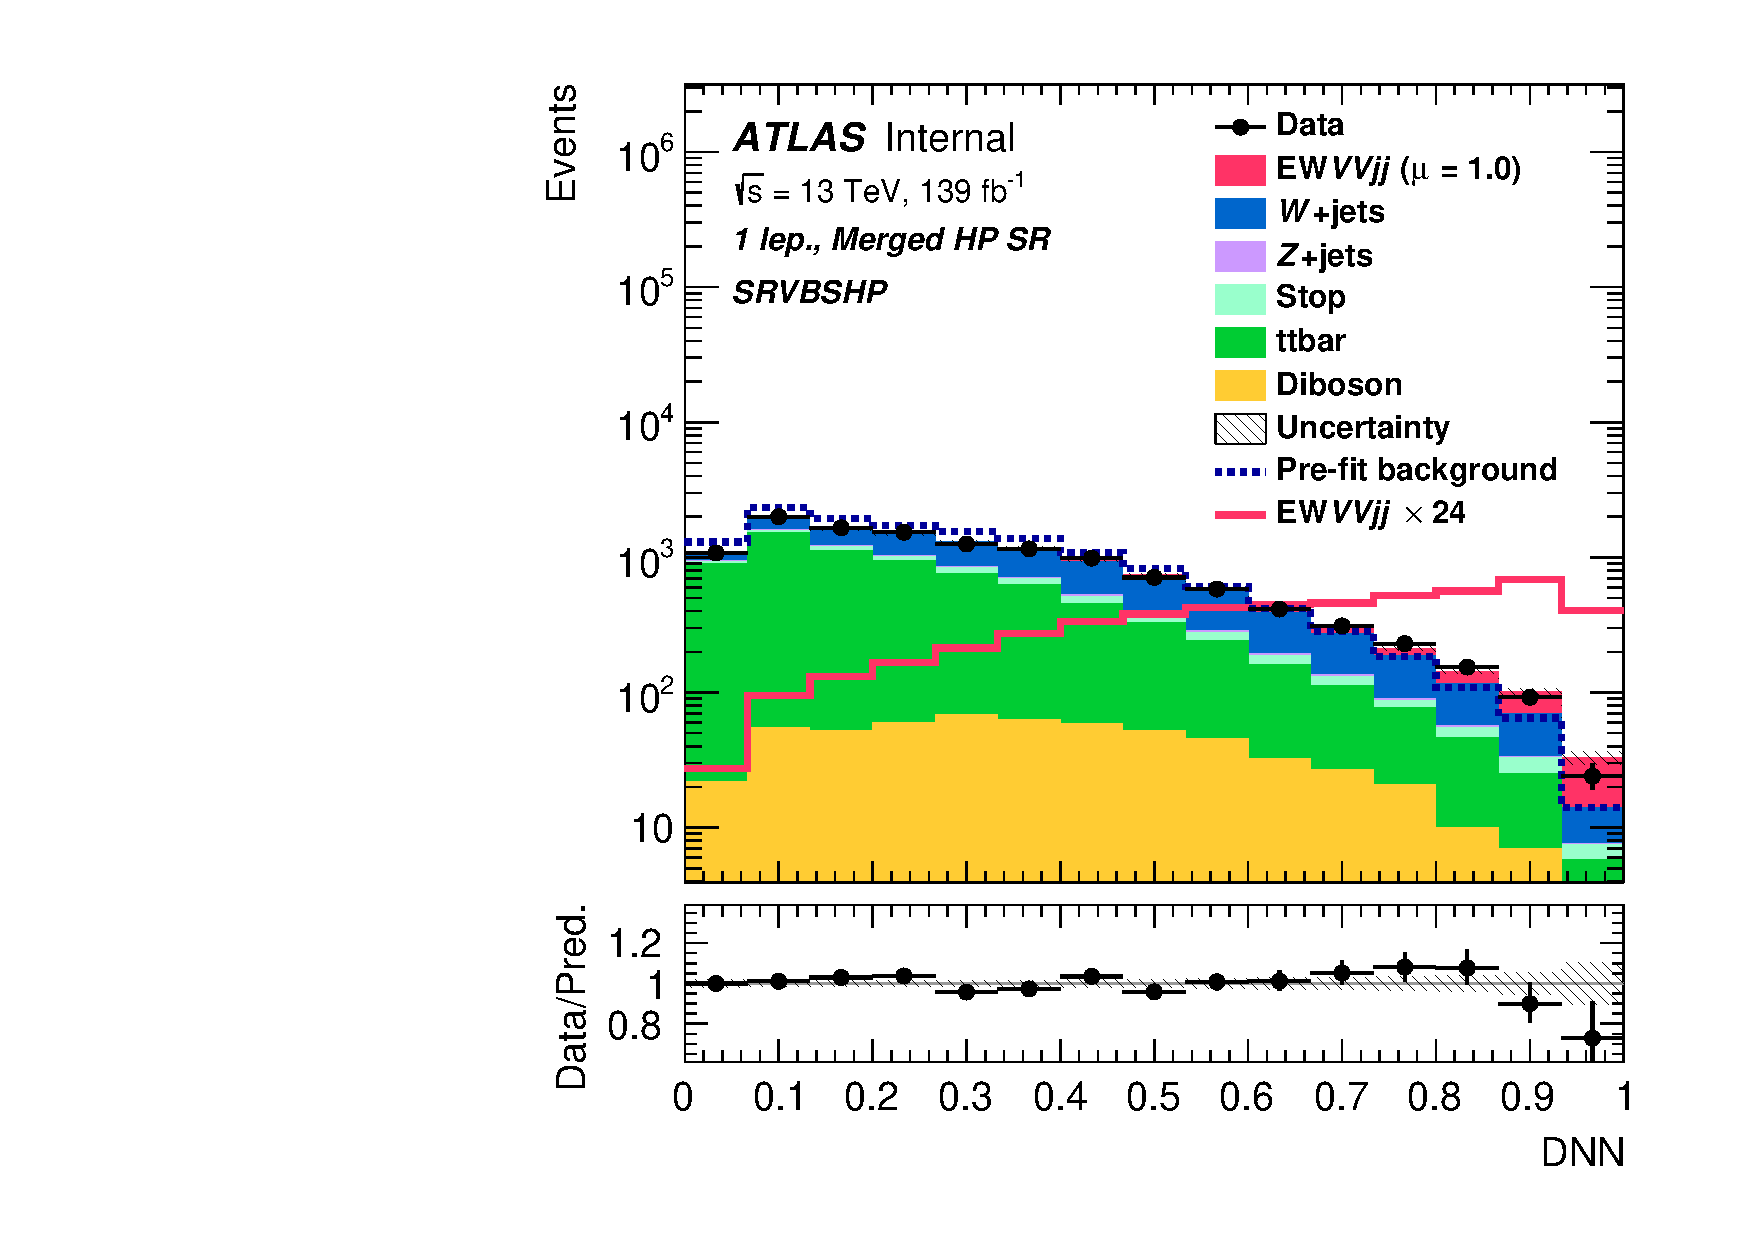
\includegraphics[width=.3\textwidth]{figures/FitResults/postfit/Region_distDNN_DSRVBSHP_BMin0_J0_incJet1_L1_T0_incFat1_Y6051_incTag1_Fat1_GlobalFit_unconditionnal_mu1log.pdf}
  }
  \subfloat[Merged LP]{
    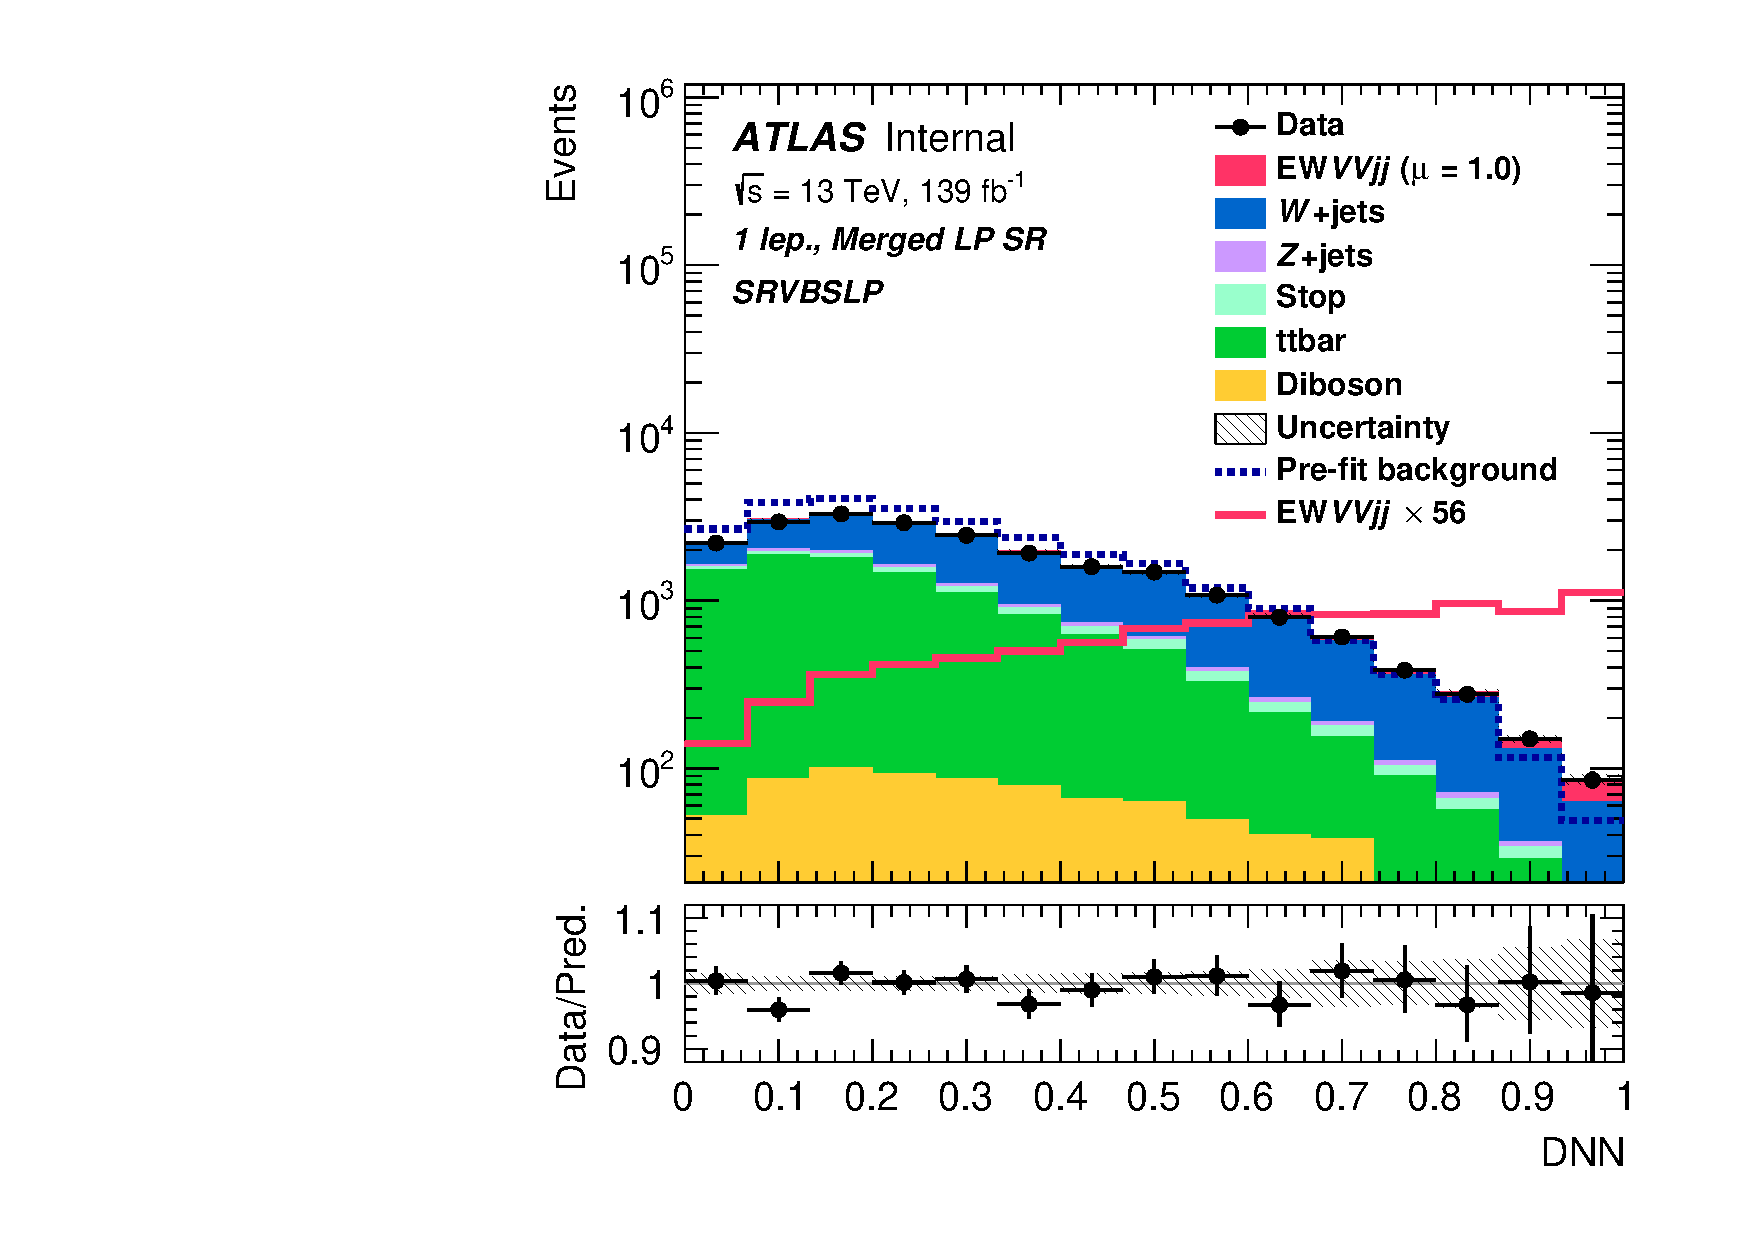
\includegraphics[width=.3\textwidth]{figures/FitResults/postfit/Region_distDNN_DSRVBSLP_BMin0_J0_incJet1_L1_T0_incFat1_Y6051_incTag1_Fat1_GlobalFit_unconditionnal_mu1log.pdf}
  }
  \subfloat[Resolved]{
    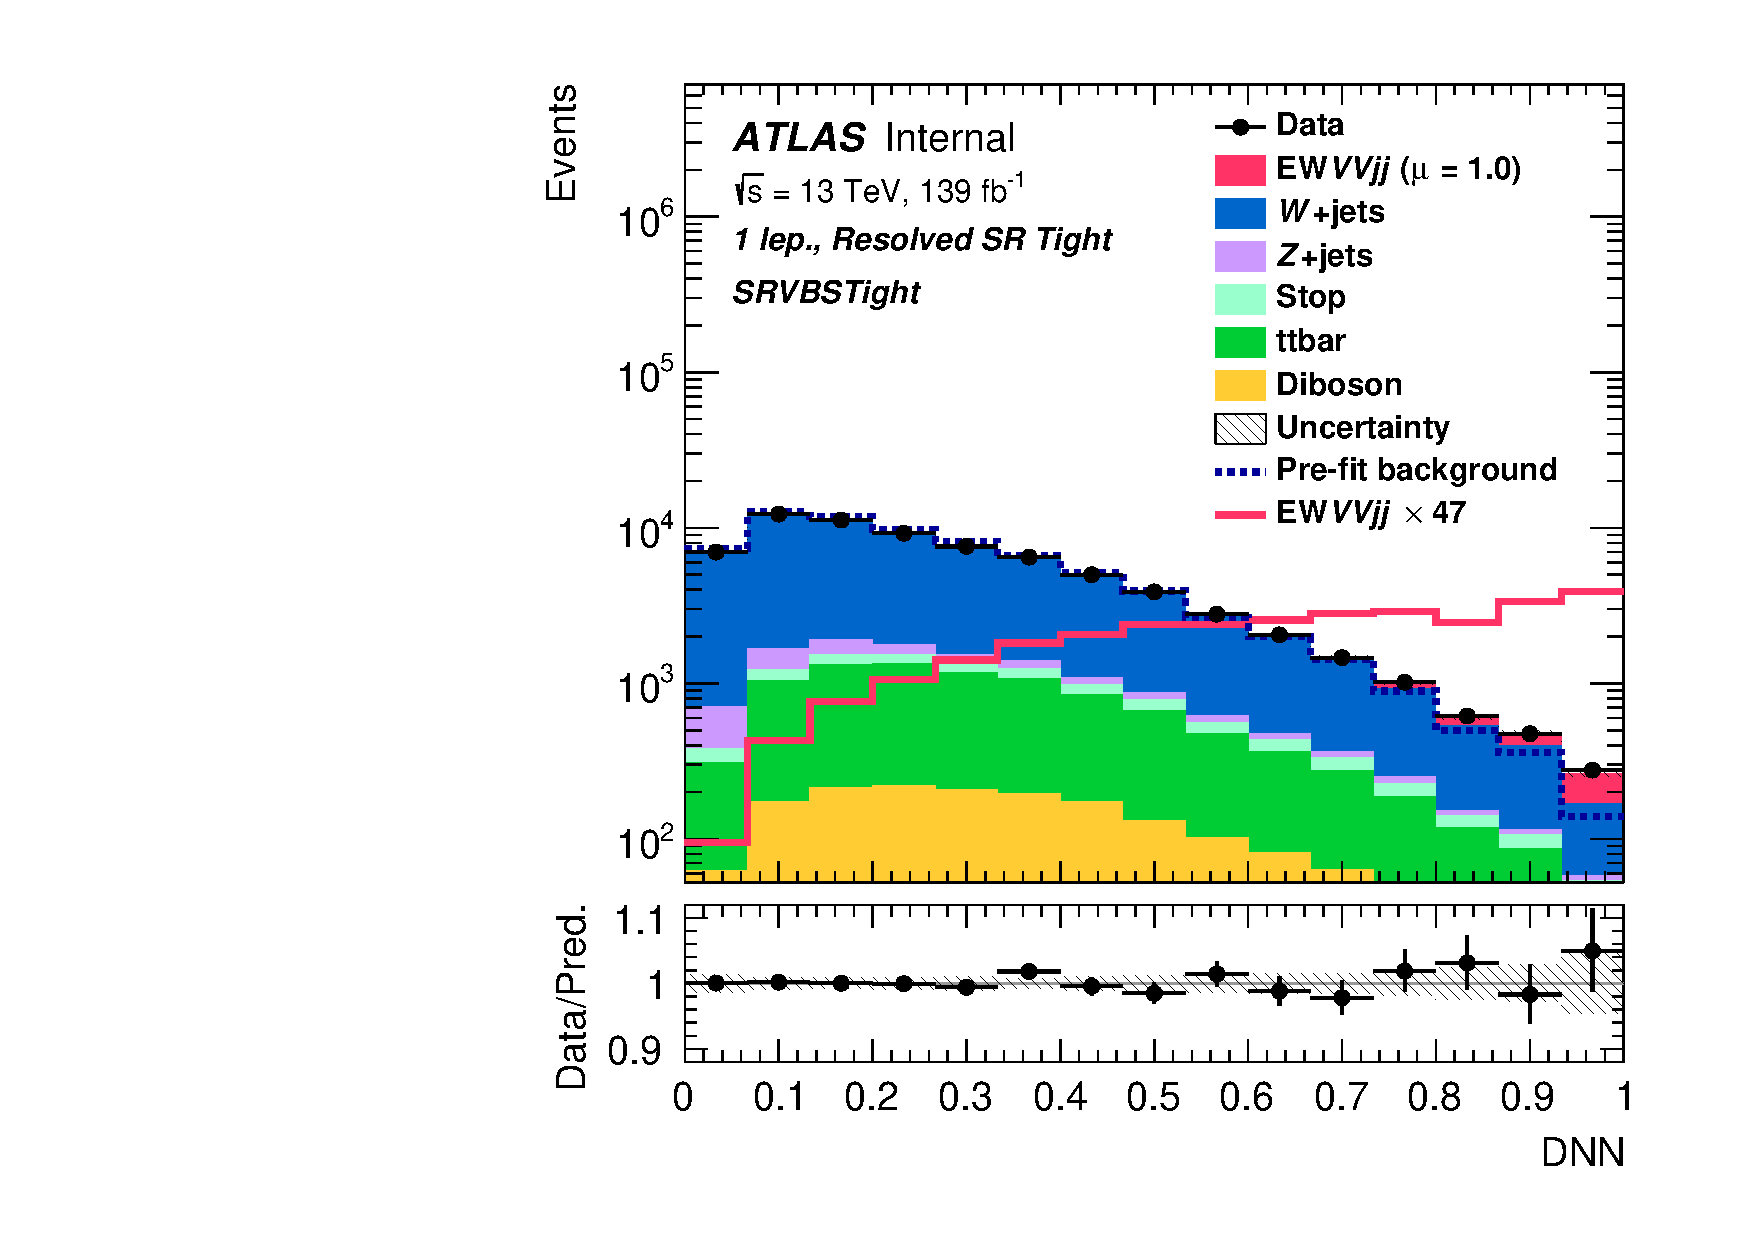
\includegraphics[width=.3\textwidth]{figures/FitResults/postfit/Region_distDNN_DSRVBSTight_BMin0_T0_Y6051_incTag1_J2_L1_incJet1_GlobalFit_unconditionnal_mu1log.pdf}
  }
  \caption{Post-fit plots for SR distributions}
  \label{fig:postfitsr_1lepdnn}
\end{figure}

\begin{figure}[h]
  \centering

  \subfloat[Resolved Top CR]{
    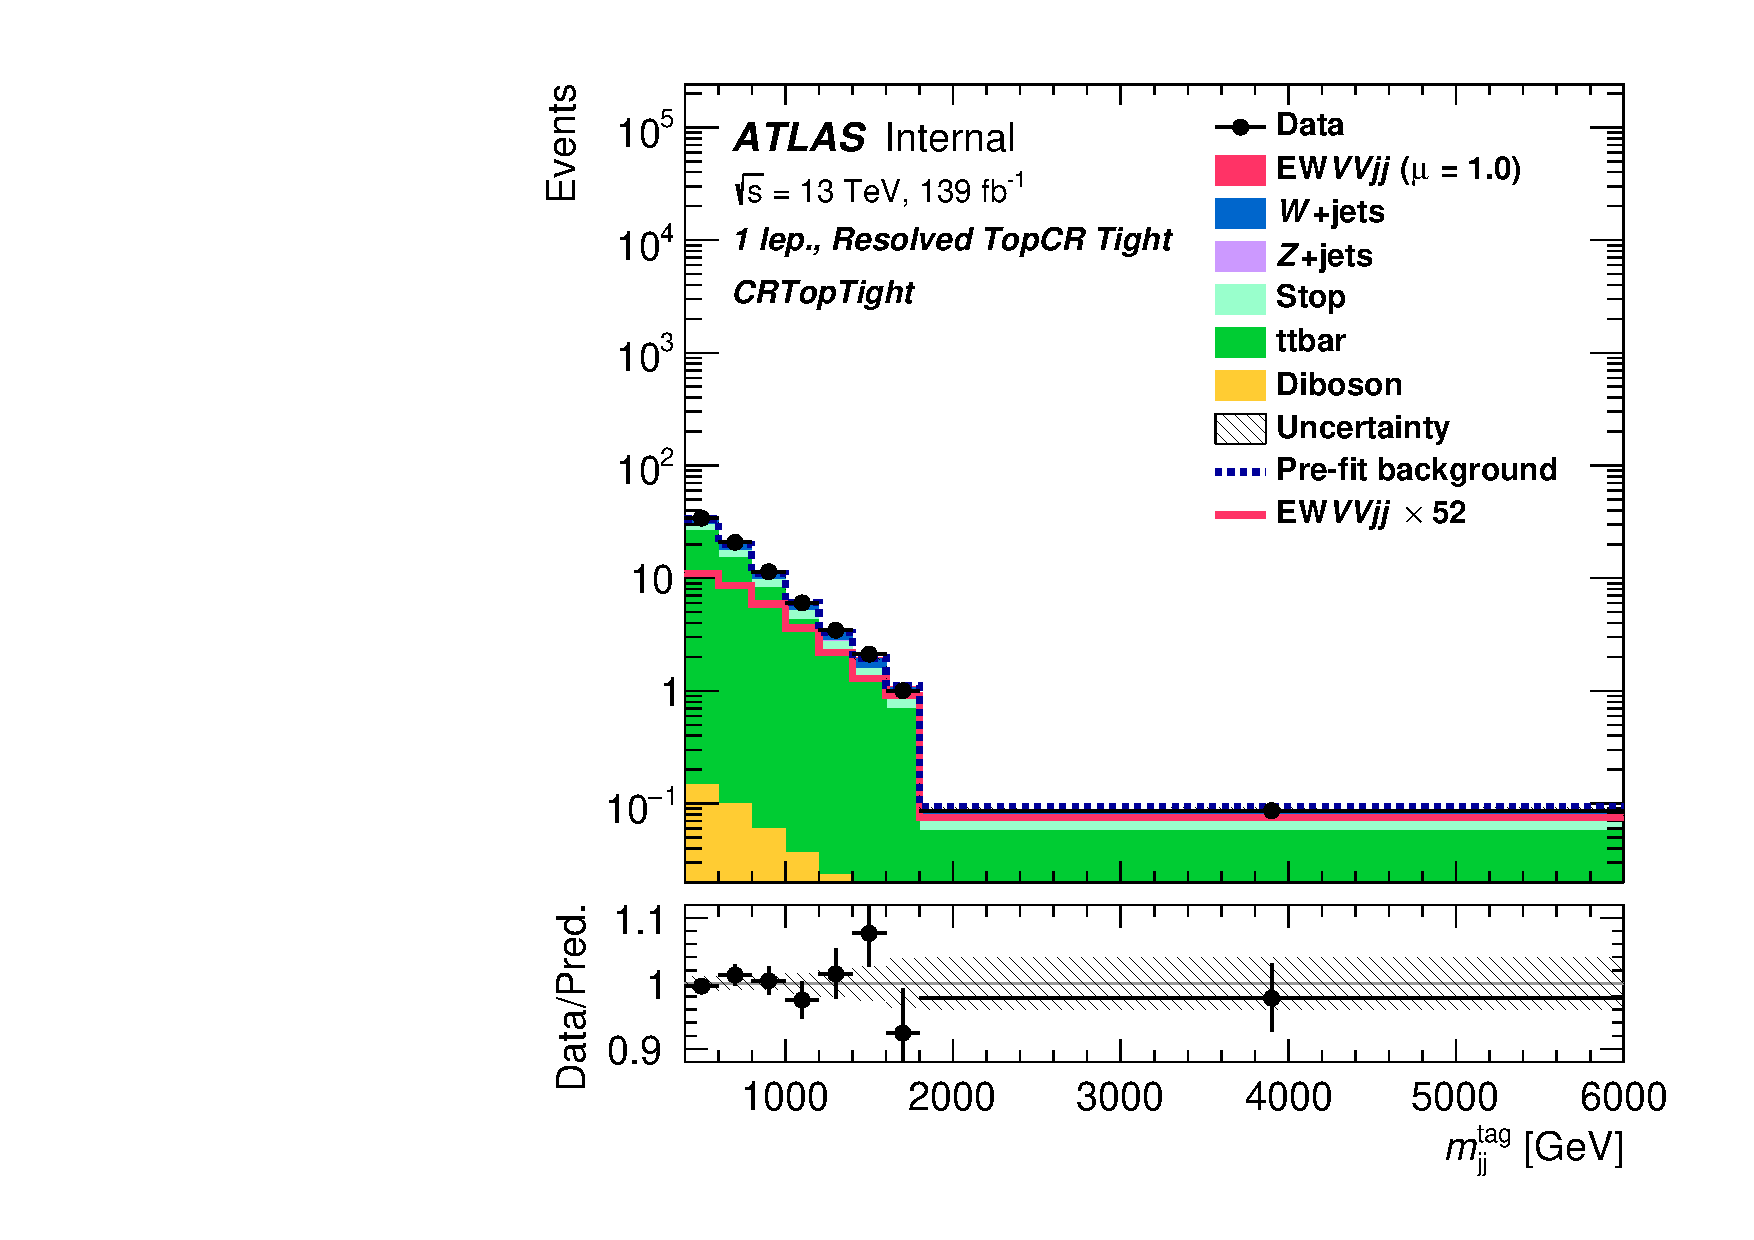
\includegraphics[width=.3\textwidth]{figures/FitResults/postfit/Region_disttagMjj_DCRTopTight_BMin0_T0_Y6051_incTag1_J2_L1_incJet1_GlobalFit_unconditionnal_mu1log.pdf}
  }
  \subfloat[Resolved Wjet CR]{
    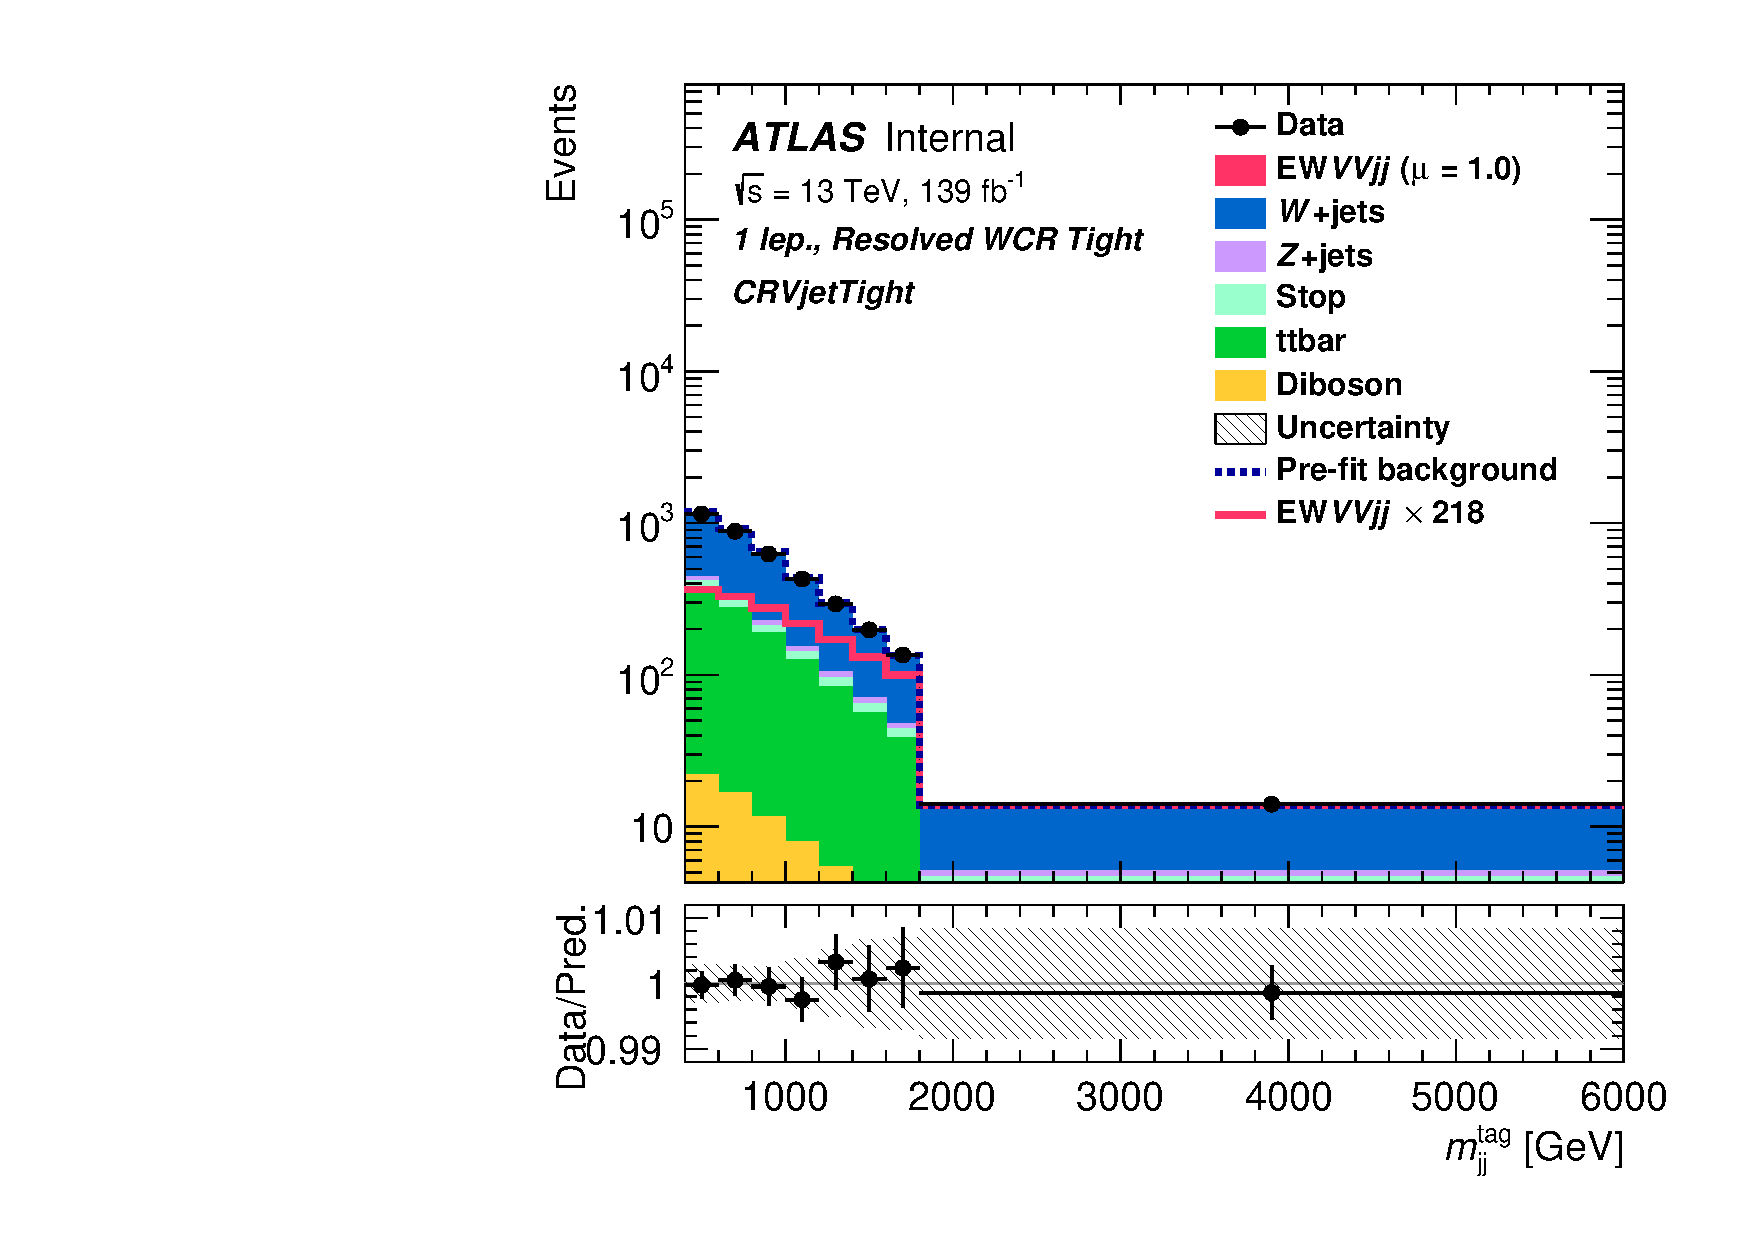
\includegraphics[width=.3\textwidth]{figures/FitResults/postfit/Region_disttagMjj_DCRVjetTight_BMin0_T0_Y6051_incTag1_J2_L1_incJet1_GlobalFit_unconditionnal_mu1log.pdf}
  }
  \subfloat[Merged Wjet CR]{
    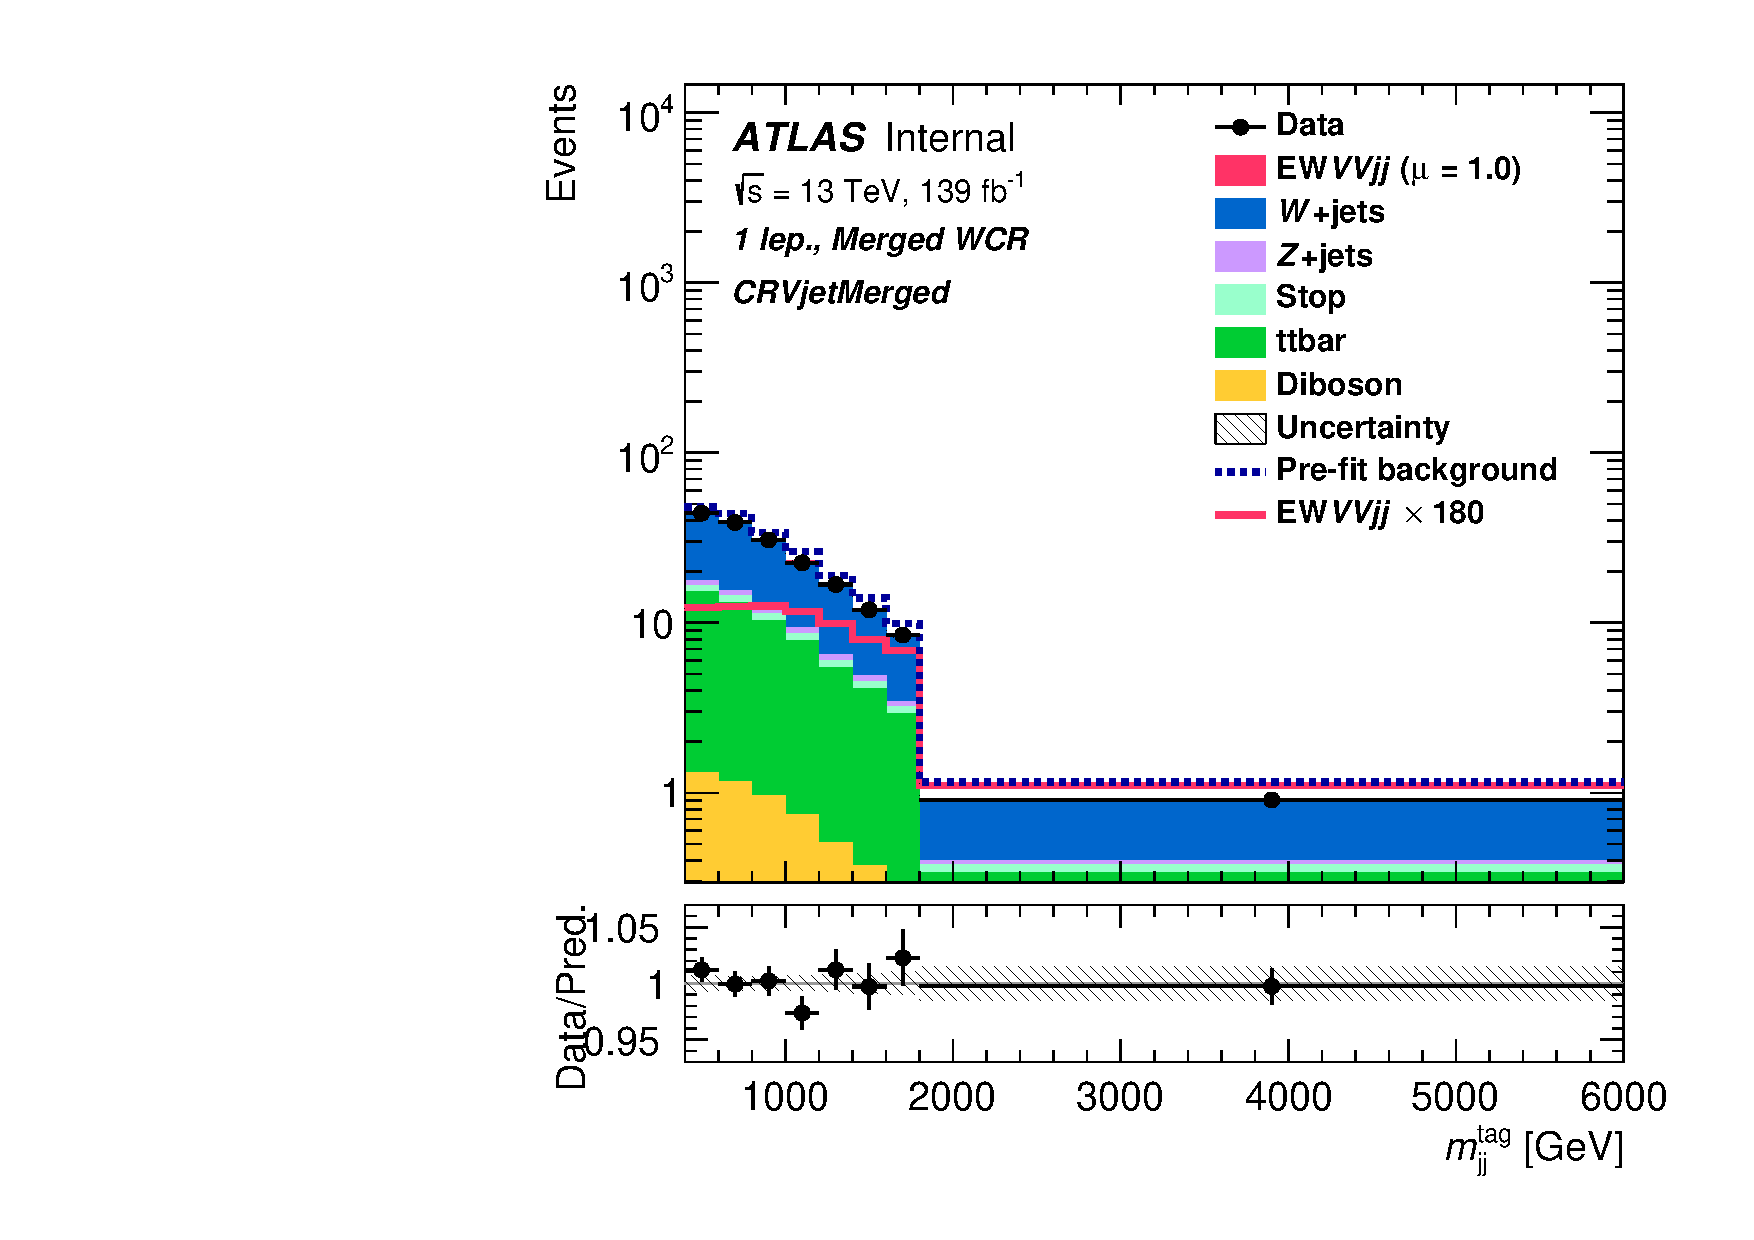
\includegraphics[width=.3\textwidth]{figures/FitResults/postfit/Region_disttagMjj_DCRVjetMerged_BMin0_J0_incJet1_L1_T0_incFat1_Y6051_incTag1_Fat1_GlobalFit_unconditionnal_mu1log.pdf}
  }

  \subfloat[Merged LP Top CR]{
    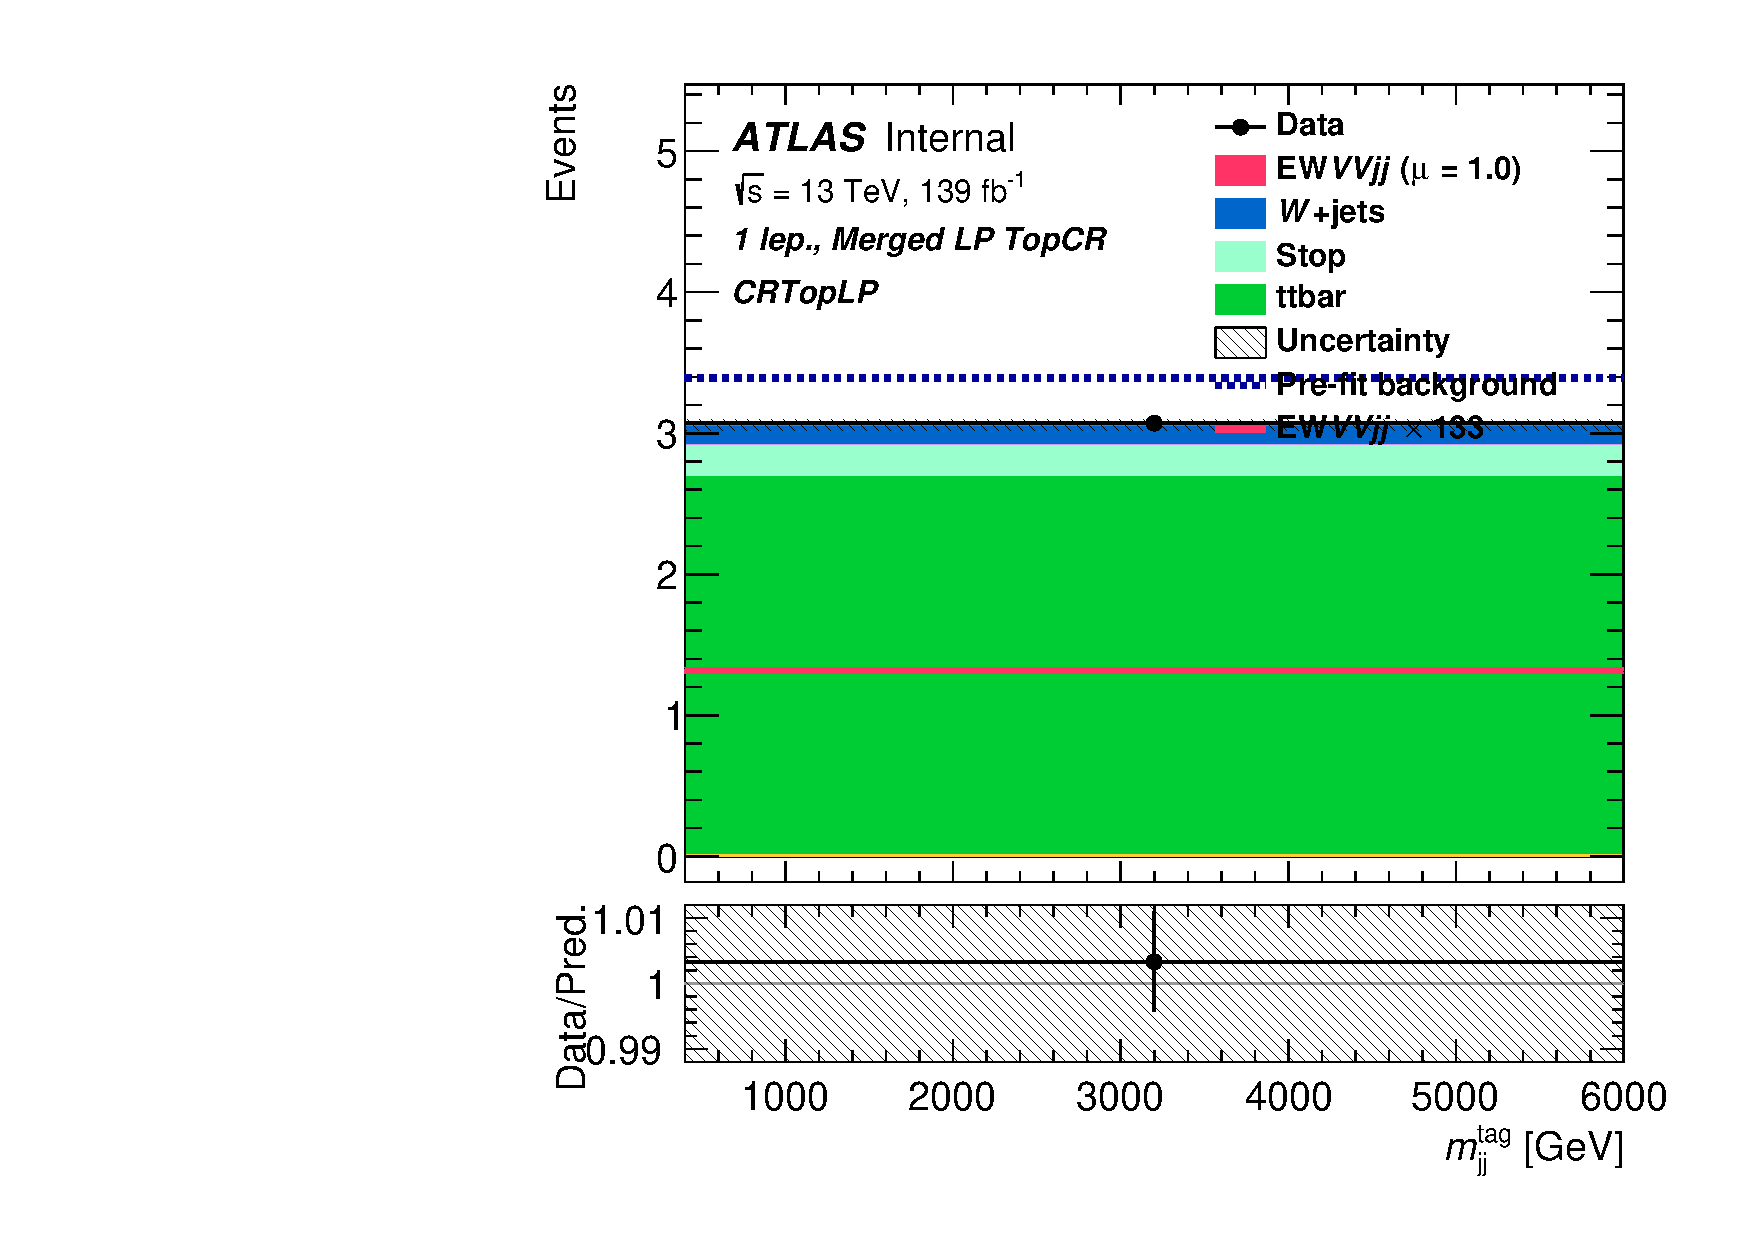
\includegraphics[width=.3\textwidth]{figures/FitResults/postfit/Region_disttagMjj_DCRTopLP_BMin0_J0_incJet1_L1_T0_incFat1_Y6051_incTag1_Fat1_GlobalFit_unconditionnal_mu1.pdf}
  }
  \subfloat[Merged HP Top CR]{
    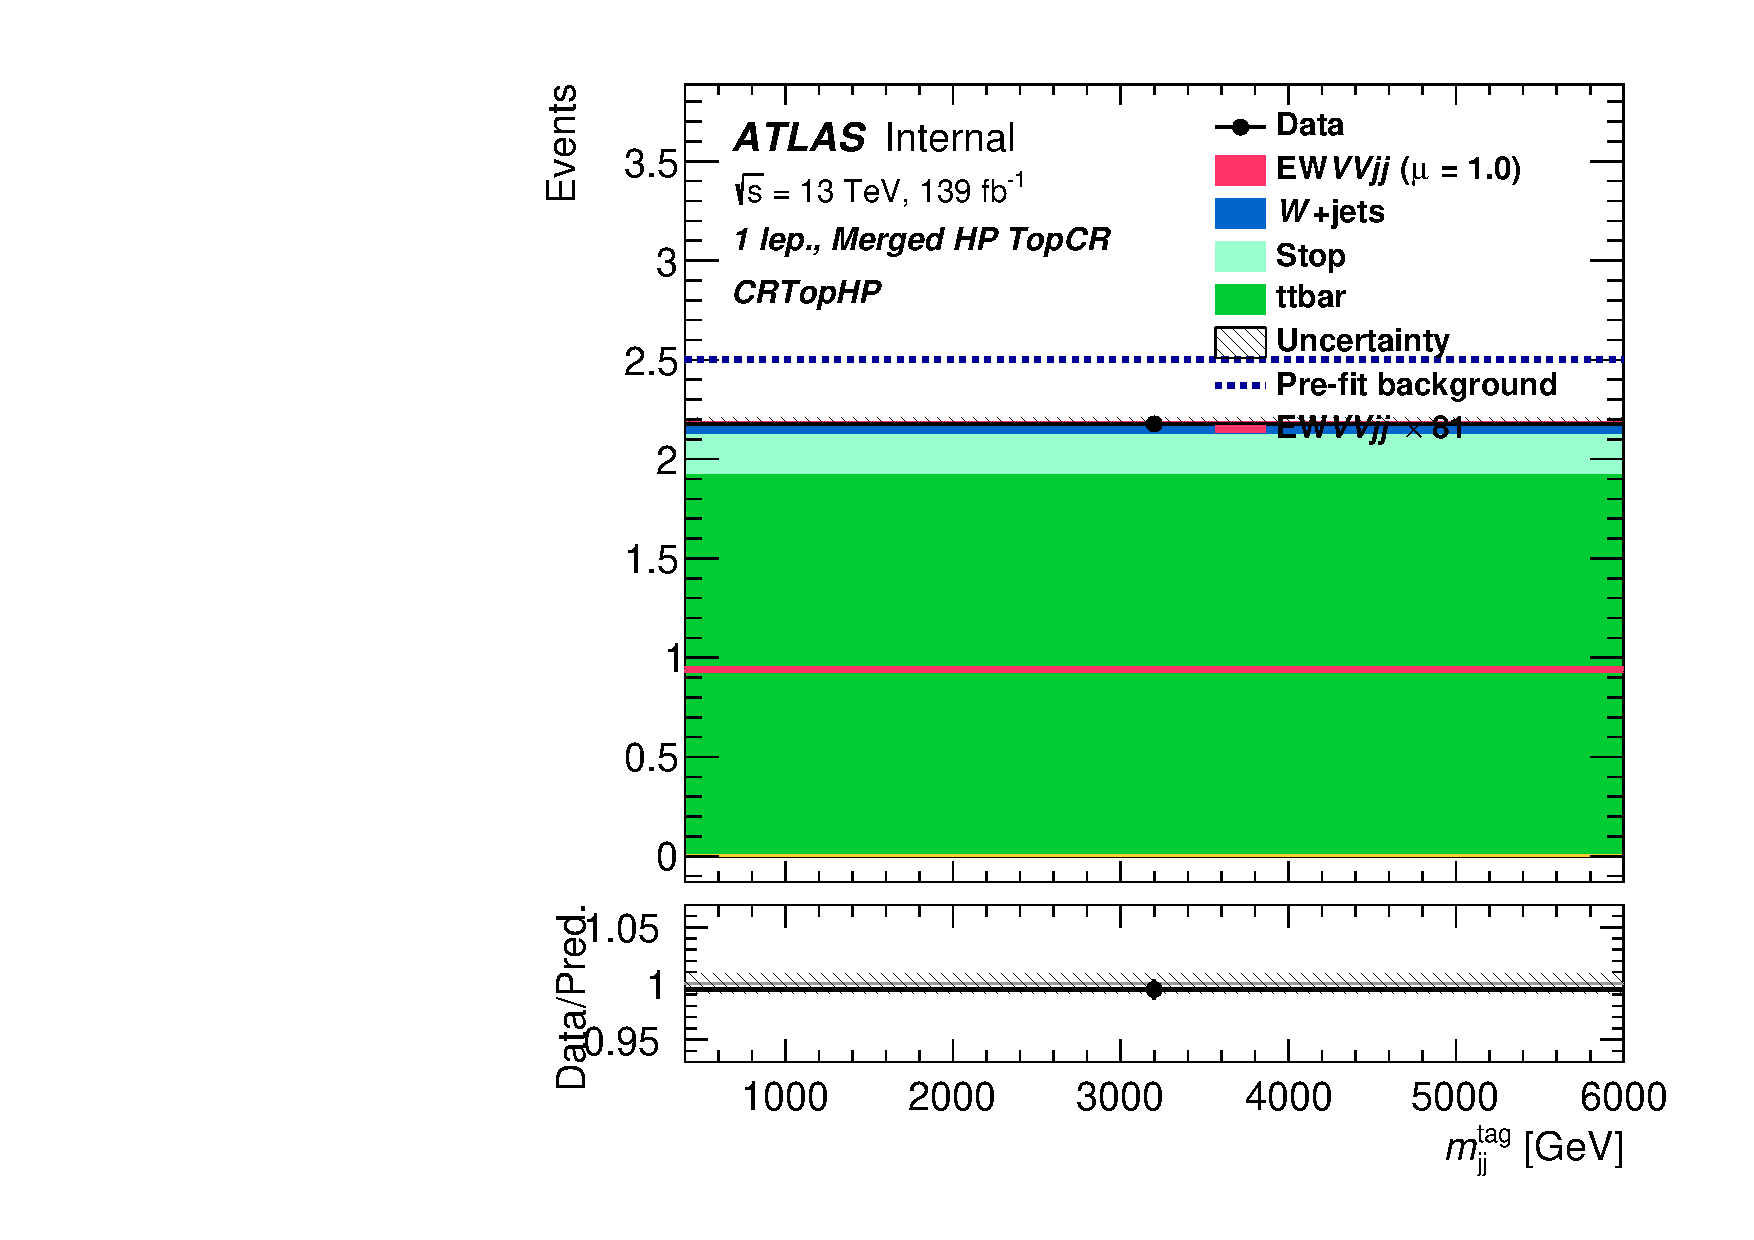
\includegraphics[width=.3\textwidth]{figures/FitResults/postfit/Region_disttagMjj_DCRTopHP_BMin0_J0_incJet1_L1_T0_incFat1_Y6051_incTag1_Fat1_GlobalFit_unconditionnal_mu1.pdf}
  }

  \caption{Post-fit plots for CR distributions}
  \label{fig:postfitcr_1lepdnn}
\end{figure}

Tables \ref{tab:1lepPostfitYield_SR}-\ref{tab:1lepPostfitYield_CR} shows the post-fit event yields for signal and background processes
in all the control and signal regions for the \olep channel.
Table \ref{tab:break_1lepdnn} shows the uncertainty breakdown on $\mu_{VBS}$.

%%%%%%%postfit_table
% \newcolumntype{d}{D{+}{\hspace{-3pt}\;\pm\;}{-1}}
%%%\documentclass{article}
%%%\usepackage{graphicx}
%%%\newcommand{\GeV}{\mathrm{GeV}}
%%%\newcommand{\ptv}{p_T^V}
%%%\begin{document}
\begin{table}
\centering
\small
\begin{tabular}{|l|c|}
\hline
 \multicolumn{2}{|c|}{DNN\_SRVBSHP}\\ \hline
W & 3772.48 $\pm$ 207.54\\
Z & 175.98 $\pm$ 24.93\\
Diboson & 574.86 $\pm$ 163.38\\
stop & 598.20 $\pm$ 167.59\\
ttbar & 6748.42 $\pm$ 277.01\\
\hline
Bkg & 11869.94 $\pm$ 110.89\\
\hline
EW6lvqq & 239.21 $\pm$ 42.47\\
\hline
Signal & 239.21 $\pm$ 42.47\\
SignalExpected & 206.48 $\pm$ 36.66\\
\hline
S/B & 2.02e-02\\
S/sqrt(S+B) & 2.17e+00\\
\hline
data & 12178\\ \hline
\end{tabular}
%%%\end{table}
%%%
%%%
%%%\begin{table}
%%%\centering
%%%\small
\begin{tabular}{|l|c|}
\hline
 \multicolumn{2}{|c|}{DNN\_SRVBSLP}\\ \hline
W & 10111.99 $\pm$ 371.67\\
Z & 462.53 $\pm$ 58.40\\
Diboson & 804.42 $\pm$ 231.65\\
stop & 846.84 $\pm$ 244.44\\
ttbar & 9856.21 $\pm$ 356.81\\
\hline
Bkg & 22082.00 $\pm$ 171.45\\
\hline
EW6lvqq & 195.86 $\pm$ 43.72\\
\hline
Signal & 195.86 $\pm$ 43.72\\
SignalExpected & 169.06 $\pm$ 37.74\\
\hline
S/B & 8.87e-03\\
S/sqrt(S+B) & 1.31e+00\\
\hline
data & 22158\\ \hline
\end{tabular}
%%%\end{table}
%%%
%%%
%%%\begin{table}
%%%\centering
%%%\small
\begin{tabular}{|l|c|}
\hline
 \multicolumn{2}{|c|}{DNN\_SRVBSRes}\\ \hline
W & 57446.51 $\pm$ 785.36\\
Z & 2168.91 $\pm$ 324.79\\
Diboson & 1721.91 $\pm$ 552.18\\
stop & 1521.92 $\pm$ 416.17\\
ttbar & 7633.82 $\pm$ 382.92\\
\hline
Bkg & 70493.07 $\pm$ 317.65\\
\hline
EW6lvqq & 742.72 $\pm$ 133.71\\
\hline
Signal & 742.72 $\pm$ 133.71\\
SignalExpected & 641.09 $\pm$ 115.41\\
\hline
S/B & 1.05e-02\\
S/sqrt(S+B) & 2.78e+00\\
\hline
data & 71272\\ \hline
\end{tabular}
\caption{Postfit event yields for the analysis SRs in the 1 lepton channel.}
\label{tab:1lepPostfitYield_SR}
\end{table}


\begin{table}
\centering
\small
\begin{tabular}{|l|c|}
\hline
 \multicolumn{2}{|c|}{tagMjj\_CRTopHP}\\ \hline
W & 279.58 $\pm$ 16.61\\
Z & 18.94 $\pm$ 2.83\\
Diboson & 46.59 $\pm$ 13.86\\
stop & 1113.16 $\pm$ 307.91\\
ttbar & 10728.53 $\pm$ 343.94\\
\hline
Bkg & 12186.80 $\pm$ 109.43\\
\hline
EW6lvqq & 74.71 $\pm$ 14.77\\
\hline
Signal & 74.71 $\pm$ 14.77\\
SignalExpected & 64.48 $\pm$ 12.75\\
\hline
S/B & 6.13e-03\\
S/sqrt(S+B) & 6.75e-01\\
\hline
data & 12195\\ \hline
\end{tabular}
%%%\end{table}
%%%
%%%
%%%\begin{table}
%%%\centering
%%%\small
\begin{tabular}{|l|c|}
\hline
 \multicolumn{2}{|c|}{tagMjj\_CRTopLP}\\ \hline
W & 717.29 $\pm$ 36.10\\
Z & 47.45 $\pm$ 6.56\\
Diboson & 68.76 $\pm$ 19.33\\
stop & 1227.37 $\pm$ 363.11\\
ttbar & 15013.46 $\pm$ 390.23\\
\hline
Bkg & 17074.34 $\pm$ 212.66\\
\hline
EW6lvqq & 63.89 $\pm$ 14.29\\
\hline
Signal & 63.89 $\pm$ 14.29\\
SignalExpected & 55.15 $\pm$ 12.33\\
\hline
S/B & 3.74e-03\\
S/sqrt(S+B) & 4.88e-01\\
\hline
data & 17195\\ \hline
\end{tabular}
%%%\end{table}
%%%
%%%
%%%\clearpage
%%%
%%%
%%%\begin{table}
%%%\centering
%%%\small
\begin{tabular}{|l|c|}
\hline
 \multicolumn{2}{|c|}{tagMjj\_CRTopRes}\\ \hline
W & 2044.50 $\pm$ 71.00\\
Z & 101.67 $\pm$ 15.16\\
Diboson & 81.79 $\pm$ 26.43\\
stop & 1885.19 $\pm$ 514.80\\
ttbar & 11853.62 $\pm$ 565.44\\
\hline
Bkg & 15966.76 $\pm$ 138.04\\
\hline
EW6lvqq & 155.57 $\pm$ 31.27\\
\hline
Signal & 155.57 $\pm$ 31.27\\
SignalExpected & 134.28 $\pm$ 26.99\\
\hline
S/B & 9.74e-03\\
S/sqrt(S+B) & 1.23e+00\\
\hline
data & 16137\\ \hline
\end{tabular}
%%%\end{table}
%%%
%%%
%%%\begin{table}
%%%\centering
%%%\small
\begin{tabular}{|l|c|}
\hline
 \multicolumn{2}{|c|}{tagMjj\_CRWjetMerged}\\ \hline
W & 22644.17 $\pm$ 842.49\\
Z & 1147.58 $\pm$ 146.40\\
Diboson & 1225.46 $\pm$ 347.60\\
stop & 1294.60 $\pm$ 360.16\\
ttbar & 11995.36 $\pm$ 787.80\\
\hline
Bkg & 38307.18 $\pm$ 211.01\\
\hline
EW6lvqq & 124.40 $\pm$ 23.18\\
\hline
Signal & 124.40 $\pm$ 23.18\\
SignalExpected & 107.37 $\pm$ 20.01\\
\hline
S/B & 3.25e-03\\
S/sqrt(S+B) & 6.35e-01\\
\hline
data & 38486\\ \hline
\end{tabular}
%%%\end{table}
%%%
%%%
%%%\begin{table}
%%%\centering
%%%\small
\begin{tabular}{|l|c|}
\hline
 \multicolumn{2}{|c|}{tagMjj\_CRWjetRes}\\ \hline
W & 501272.25 $\pm$ 9637.60\\
Z & 21630.23 $\pm$ 3315.37\\
Diboson & 15241.39 $\pm$ 4878.27\\
stop & 29343.00 $\pm$ 8099.30\\
ttbar & 231974.93 $\pm$ 10369.58\\
\hline
Bkg & 799461.79 $\pm$ 2665.92\\
\hline
EW6lvqq & 1989.35 $\pm$ 394.05\\
\hline
Signal & 1989.35 $\pm$ 394.05\\
SignalExpected & 1717.15 $\pm$ 340.13\\
\hline
S/B & 2.49e-03\\
S/sqrt(S+B) & 2.22e+00\\
\hline
data & 801406\\ \hline
\end{tabular}
\caption{Postfit event yields for the analysis CRs in the 1 lepton channel.}
\label{tab:1lepPostfitYield_CR}
\end{table}


%%%\end{document}


\begin{table}[h]
\centering
\begin{tabular}{|l|c|c|c|}
\hline
Total                    & \(+0.263\) & \(-0.237\) & \(\pm 0.250\) \\
DataStat                 & \(+0.107\) & \(-0.105\) & \(\pm 0.106\) \\
FullSyst                 & \(+0.240\) & \(-0.212\) & \(\pm 0.226\) \\
\hline
Floating normalizations  & \(+0.044\) & \(-0.035\) & \(\pm 0.039\) \\
All normalizations       & \(+0.095\) & \(-0.079\) & \(\pm 0.087\) \\
All but normalizations   & \(+0.230\) & \(-0.202\) & \(\pm 0.216\) \\
Jets MET                 & \(+0.132\) & \(-0.118\) & \(\pm 0.125\) \\
BTag                     & \(+0.031\) & \(-0.031\) & \(\pm 0.031\) \\
Leptons                  & \(+0.000\) & \(-0.000\) & \(\pm 0.000\) \\
Luminosity               & \(+0.025\) & \(-0.019\) & \(\pm 0.022\) \\
Diboson                  & \(+0.036\) & \(-0.032\) & \(\pm 0.034\) \\
Model                    & \(+0.148\) & \(-0.128\) & \(\pm 0.138\) \\
Signal Systematics       & \(+0.166\) & \(-0.133\) & \(\pm 0.150\) \\
Mjj reweighting          & \(+0.023\) & \(-0.037\) & \(\pm 0.030\) \\
Quark gluon              & \(+0.015\) & \(-0.009\) & \(\pm 0.012\) \\
MC stat                  & \(+0.082\) & \(-0.077\) & \(\pm 0.079\) \\
\hline
\end{tabular}
\caption{Uncertainty breakdown on $\mu_{VBS}$ in \olep DNN.}
\label{tab:break_1lepdnn}
\end{table}

Figure \ref{fig:fit_1lep_corr_all_data} shows the correlation matrix for full range data fit.
Figure \ref{fig:fit_1lep_fcc_data}-\ref{fig:fit_1lep_ranking_all_data} show the pulls of the NPs and the ranking plots for the unblinded full range data fit. 
The leading uncertainties impacting the fit are the theoretical QCD uncertainty on the signal, 
the modeling uncertainties of the \Wjets background,
the reweighting uncertainties of the tagging jets, 
and \texttt{SysJET\_JERComb}, the baseline uncertainties from the small-$R$ jets resolution.

%%\begin{figure}[ht]
%%      \centering
%%        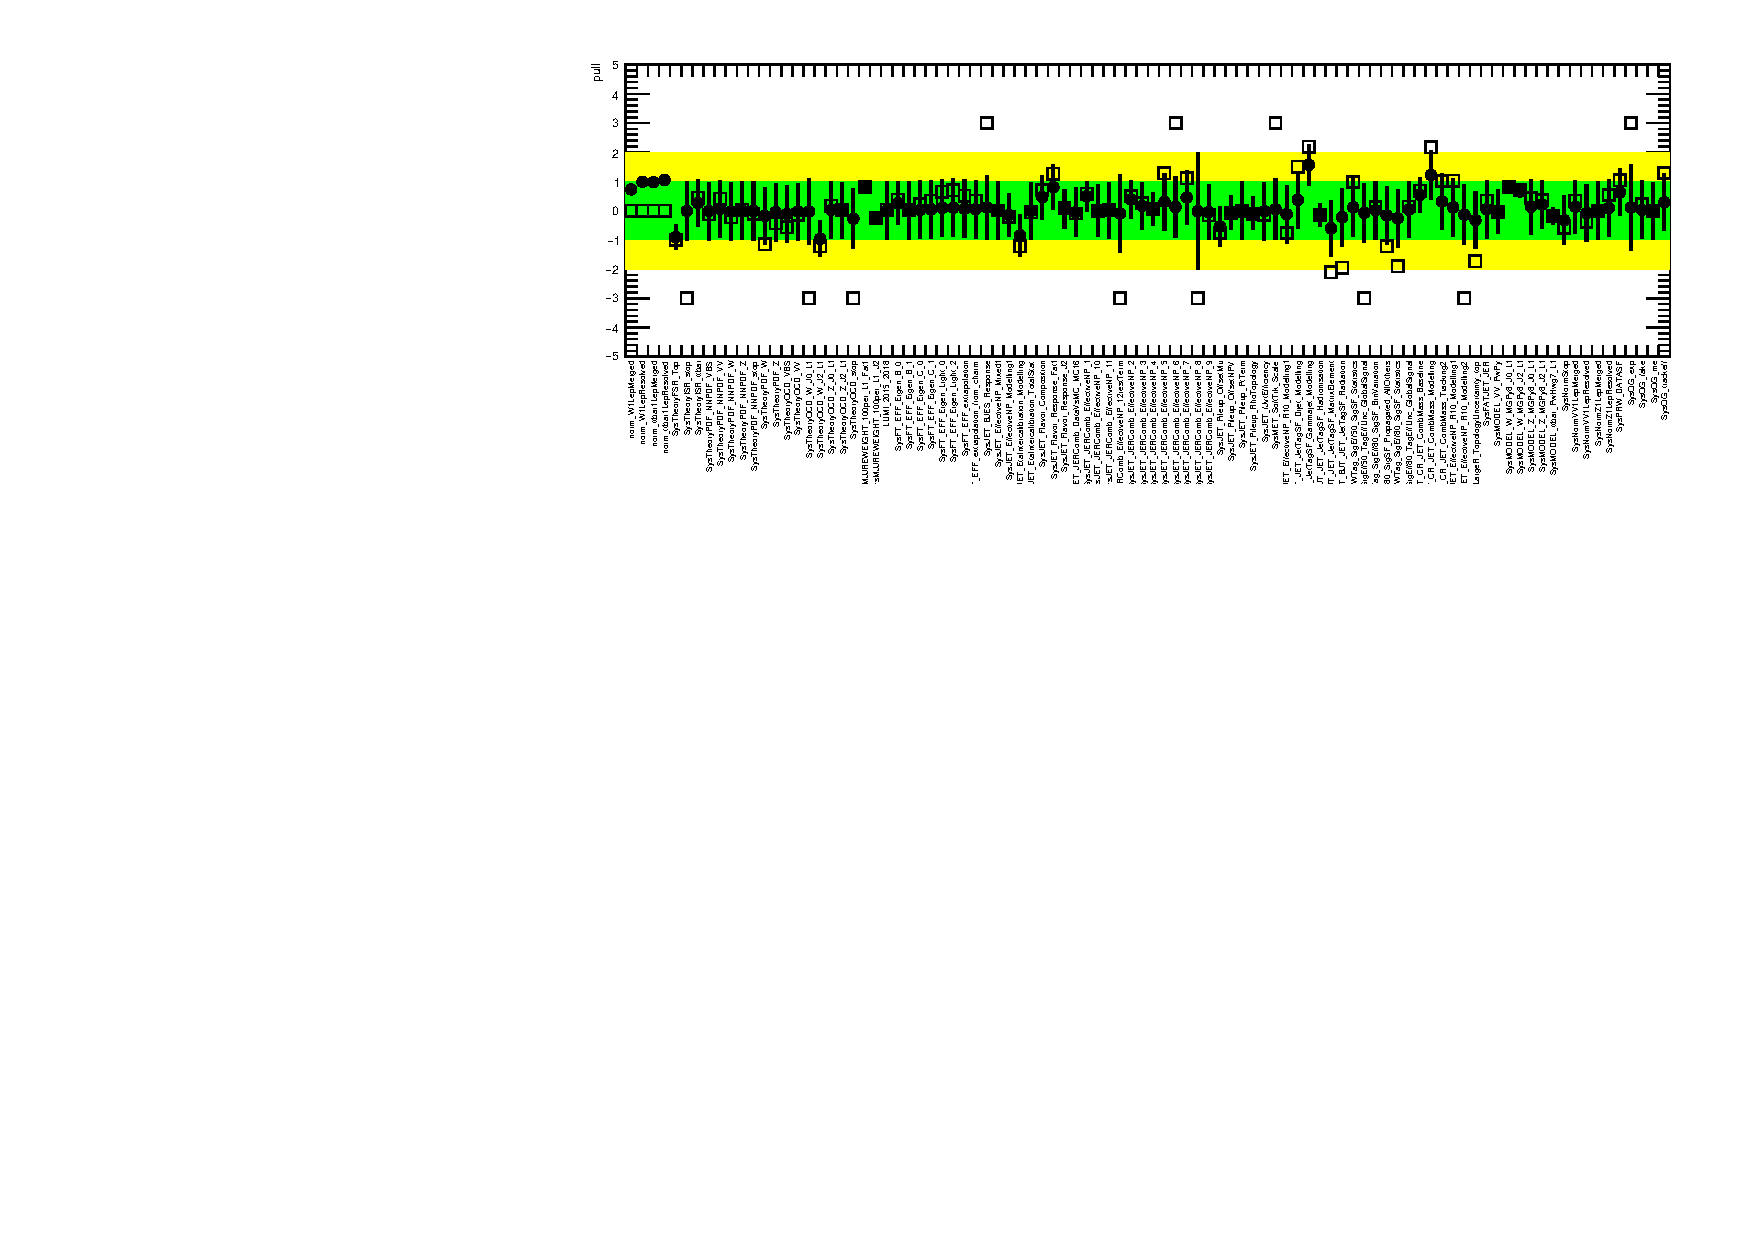
\includegraphics[width=\linewidth]{figures/Fit_fcc/GlobalFit/NP_allExceptGammas.pdf}
%%        \caption{Fit cross-check, conditional fit ($\mu=1$) to asimov data for the 1 lepton channel.}
%%       \label{fig:fit_1lep_fcc_data}
%%\end{figure}

\begin{figure}[ht]
      \centering
        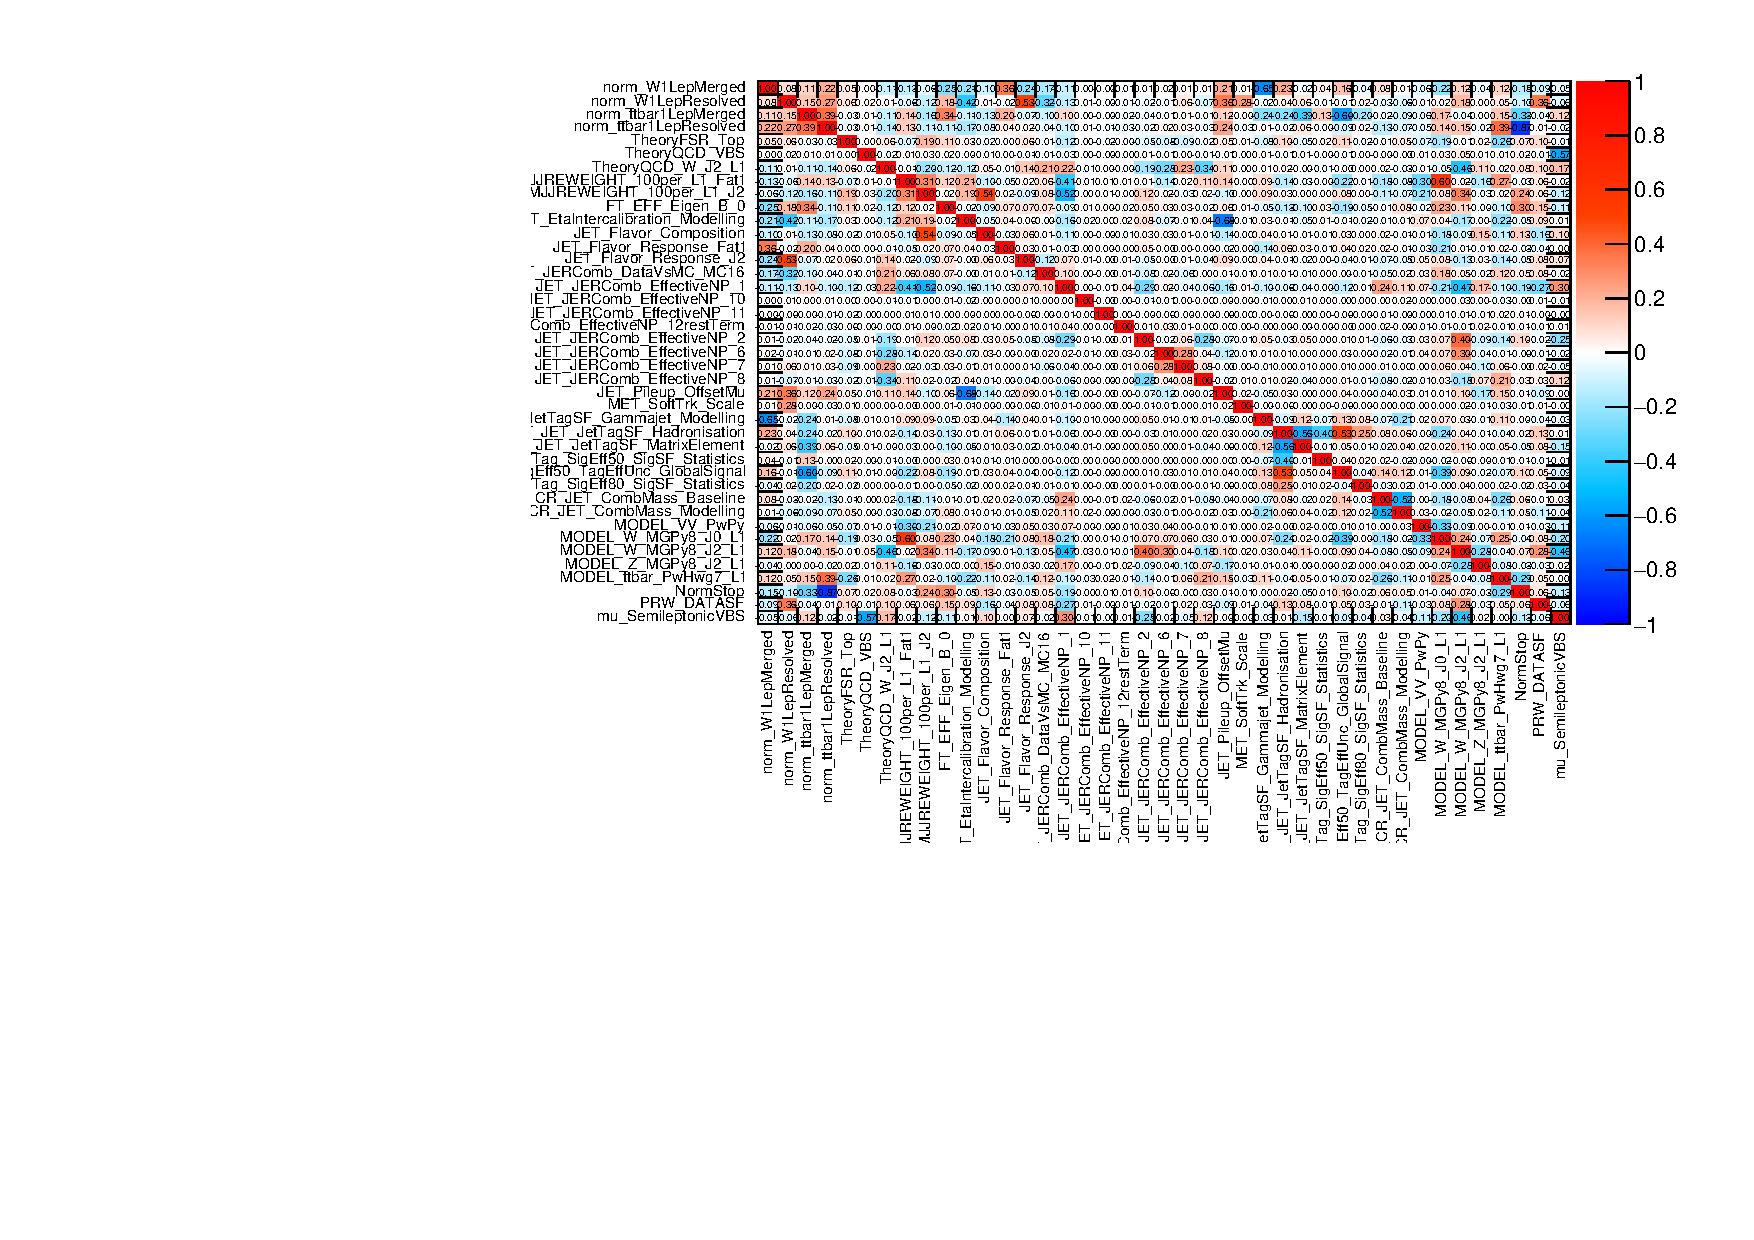
\includegraphics[width=\linewidth]{figures/Fit_fcc/GlobalFit/corr_HighCorrNoMCStat.pdf}
        \caption{Correlations for unconditional fit ($\mu=1$) to unblinded data in the full range.}
       \label{fig:fit_1lep_corr_all_data}
\end{figure}

\begin{figure}[ht]
      \centering
        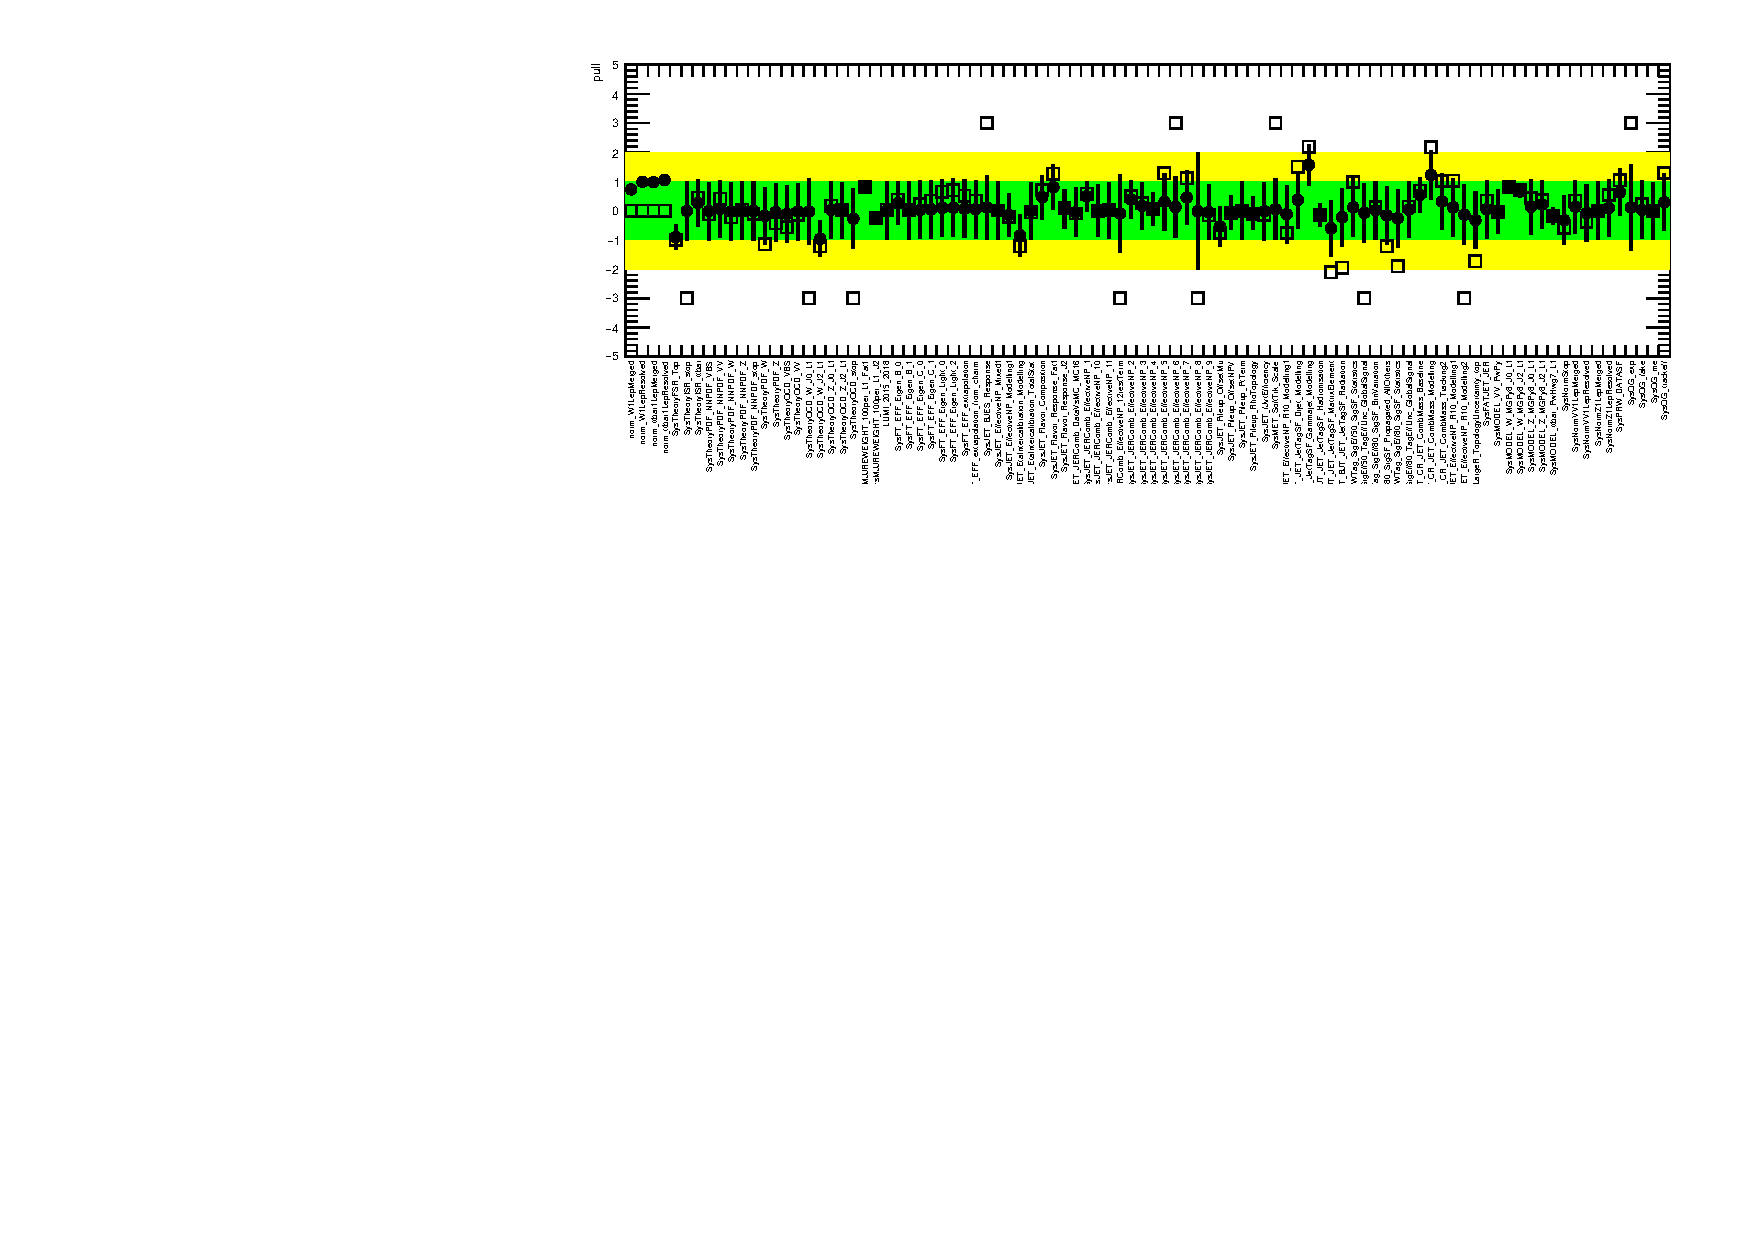
\includegraphics[width=\linewidth]{figures/Fit_fcc/GlobalFit/NP_allExceptGammas.pdf}
        \caption{Fit cross-check, the pulls of the NPs for the unblinded fit.}
       \label{fig:fit_1lep_fcc_data}
\end{figure}

\begin{figure}[ht]
      \centering
        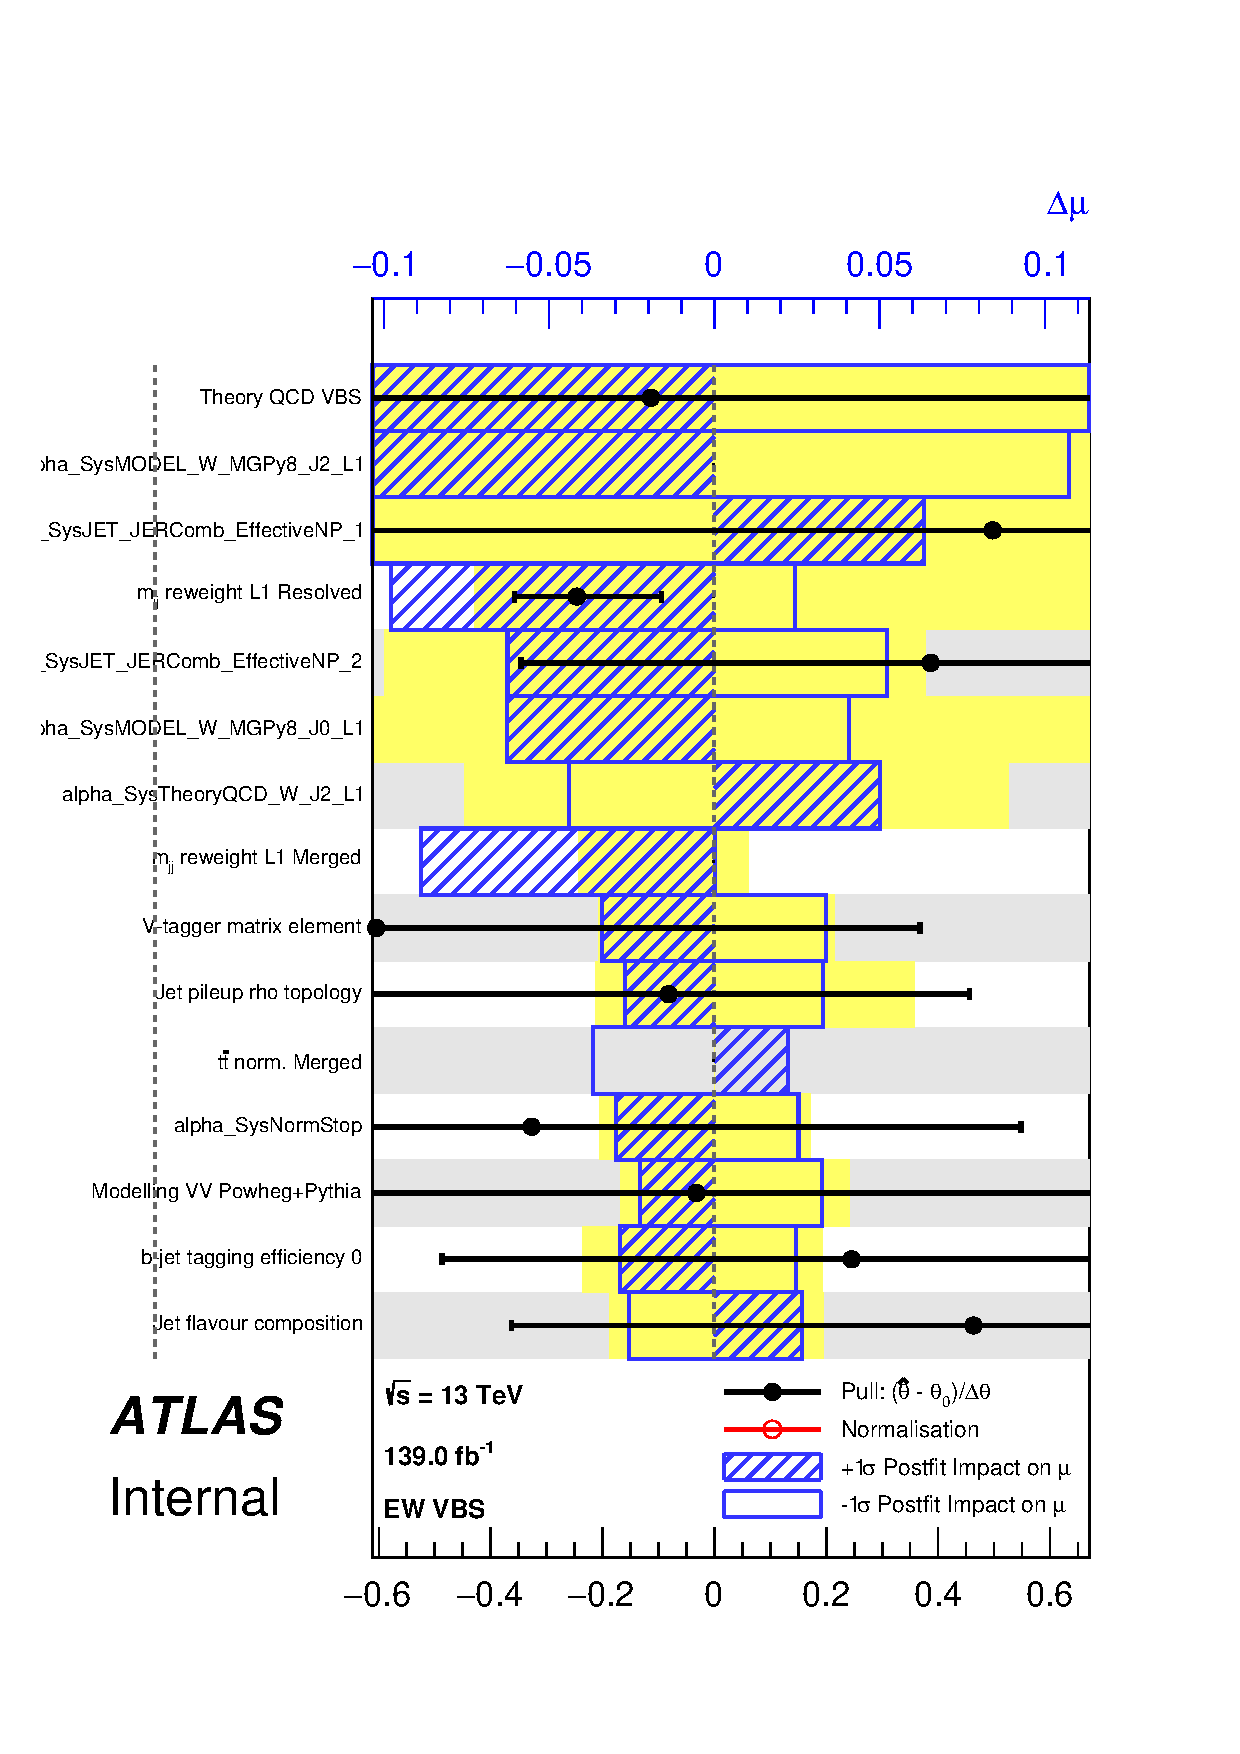
\includegraphics[width=0.5\textwidth]{figures/Fit_np_rank/pulls_mu_Global/pulls_mu_SemileptonicVBS_5.pdf}
        \caption{Ranking of nuisance parameters postfit-sorted for the unblinded fit.}
       \label{fig:fit_1lep_ranking_all_data}
\end{figure}


%%%%%%%postfit_table
%Tables \ref{tab:1lepPostfitYield_SR}-\ref{tab:1lepPostfitYield_CR} shows the expected yields for signal and background processes
%in all the control and signal regions for the \olep channel.

%% \newcolumntype{d}{D{+}{\hspace{-3pt}\;\pm\;}{-1}}
%%%\documentclass{article}
%%%\usepackage{graphicx}
%%%\newcommand{\GeV}{\mathrm{GeV}}
%%%\newcommand{\ptv}{p_T^V}
%%%\begin{document}
\begin{table}
\centering
\small
\begin{tabular}{|l|c|}
\hline
 \multicolumn{2}{|c|}{DNN\_SRVBSHP}\\ \hline
W & 3772.48 $\pm$ 207.54\\
Z & 175.98 $\pm$ 24.93\\
Diboson & 574.86 $\pm$ 163.38\\
stop & 598.20 $\pm$ 167.59\\
ttbar & 6748.42 $\pm$ 277.01\\
\hline
Bkg & 11869.94 $\pm$ 110.89\\
\hline
EW6lvqq & 239.21 $\pm$ 42.47\\
\hline
Signal & 239.21 $\pm$ 42.47\\
SignalExpected & 206.48 $\pm$ 36.66\\
\hline
S/B & 2.02e-02\\
S/sqrt(S+B) & 2.17e+00\\
\hline
data & 12178\\ \hline
\end{tabular}
%%%\end{table}
%%%
%%%
%%%\begin{table}
%%%\centering
%%%\small
\begin{tabular}{|l|c|}
\hline
 \multicolumn{2}{|c|}{DNN\_SRVBSLP}\\ \hline
W & 10111.99 $\pm$ 371.67\\
Z & 462.53 $\pm$ 58.40\\
Diboson & 804.42 $\pm$ 231.65\\
stop & 846.84 $\pm$ 244.44\\
ttbar & 9856.21 $\pm$ 356.81\\
\hline
Bkg & 22082.00 $\pm$ 171.45\\
\hline
EW6lvqq & 195.86 $\pm$ 43.72\\
\hline
Signal & 195.86 $\pm$ 43.72\\
SignalExpected & 169.06 $\pm$ 37.74\\
\hline
S/B & 8.87e-03\\
S/sqrt(S+B) & 1.31e+00\\
\hline
data & 22158\\ \hline
\end{tabular}
%%%\end{table}
%%%
%%%
%%%\begin{table}
%%%\centering
%%%\small
\begin{tabular}{|l|c|}
\hline
 \multicolumn{2}{|c|}{DNN\_SRVBSRes}\\ \hline
W & 57446.51 $\pm$ 785.36\\
Z & 2168.91 $\pm$ 324.79\\
Diboson & 1721.91 $\pm$ 552.18\\
stop & 1521.92 $\pm$ 416.17\\
ttbar & 7633.82 $\pm$ 382.92\\
\hline
Bkg & 70493.07 $\pm$ 317.65\\
\hline
EW6lvqq & 742.72 $\pm$ 133.71\\
\hline
Signal & 742.72 $\pm$ 133.71\\
SignalExpected & 641.09 $\pm$ 115.41\\
\hline
S/B & 1.05e-02\\
S/sqrt(S+B) & 2.78e+00\\
\hline
data & 71272\\ \hline
\end{tabular}
\caption{Postfit event yields for the analysis SRs in the 1 lepton channel.}
\label{tab:1lepPostfitYield_SR}
\end{table}


\begin{table}
\centering
\small
\begin{tabular}{|l|c|}
\hline
 \multicolumn{2}{|c|}{tagMjj\_CRTopHP}\\ \hline
W & 279.58 $\pm$ 16.61\\
Z & 18.94 $\pm$ 2.83\\
Diboson & 46.59 $\pm$ 13.86\\
stop & 1113.16 $\pm$ 307.91\\
ttbar & 10728.53 $\pm$ 343.94\\
\hline
Bkg & 12186.80 $\pm$ 109.43\\
\hline
EW6lvqq & 74.71 $\pm$ 14.77\\
\hline
Signal & 74.71 $\pm$ 14.77\\
SignalExpected & 64.48 $\pm$ 12.75\\
\hline
S/B & 6.13e-03\\
S/sqrt(S+B) & 6.75e-01\\
\hline
data & 12195\\ \hline
\end{tabular}
%%%\end{table}
%%%
%%%
%%%\begin{table}
%%%\centering
%%%\small
\begin{tabular}{|l|c|}
\hline
 \multicolumn{2}{|c|}{tagMjj\_CRTopLP}\\ \hline
W & 717.29 $\pm$ 36.10\\
Z & 47.45 $\pm$ 6.56\\
Diboson & 68.76 $\pm$ 19.33\\
stop & 1227.37 $\pm$ 363.11\\
ttbar & 15013.46 $\pm$ 390.23\\
\hline
Bkg & 17074.34 $\pm$ 212.66\\
\hline
EW6lvqq & 63.89 $\pm$ 14.29\\
\hline
Signal & 63.89 $\pm$ 14.29\\
SignalExpected & 55.15 $\pm$ 12.33\\
\hline
S/B & 3.74e-03\\
S/sqrt(S+B) & 4.88e-01\\
\hline
data & 17195\\ \hline
\end{tabular}
%%%\end{table}
%%%
%%%
%%%\clearpage
%%%
%%%
%%%\begin{table}
%%%\centering
%%%\small
\begin{tabular}{|l|c|}
\hline
 \multicolumn{2}{|c|}{tagMjj\_CRTopRes}\\ \hline
W & 2044.50 $\pm$ 71.00\\
Z & 101.67 $\pm$ 15.16\\
Diboson & 81.79 $\pm$ 26.43\\
stop & 1885.19 $\pm$ 514.80\\
ttbar & 11853.62 $\pm$ 565.44\\
\hline
Bkg & 15966.76 $\pm$ 138.04\\
\hline
EW6lvqq & 155.57 $\pm$ 31.27\\
\hline
Signal & 155.57 $\pm$ 31.27\\
SignalExpected & 134.28 $\pm$ 26.99\\
\hline
S/B & 9.74e-03\\
S/sqrt(S+B) & 1.23e+00\\
\hline
data & 16137\\ \hline
\end{tabular}
%%%\end{table}
%%%
%%%
%%%\begin{table}
%%%\centering
%%%\small
\begin{tabular}{|l|c|}
\hline
 \multicolumn{2}{|c|}{tagMjj\_CRWjetMerged}\\ \hline
W & 22644.17 $\pm$ 842.49\\
Z & 1147.58 $\pm$ 146.40\\
Diboson & 1225.46 $\pm$ 347.60\\
stop & 1294.60 $\pm$ 360.16\\
ttbar & 11995.36 $\pm$ 787.80\\
\hline
Bkg & 38307.18 $\pm$ 211.01\\
\hline
EW6lvqq & 124.40 $\pm$ 23.18\\
\hline
Signal & 124.40 $\pm$ 23.18\\
SignalExpected & 107.37 $\pm$ 20.01\\
\hline
S/B & 3.25e-03\\
S/sqrt(S+B) & 6.35e-01\\
\hline
data & 38486\\ \hline
\end{tabular}
%%%\end{table}
%%%
%%%
%%%\begin{table}
%%%\centering
%%%\small
\begin{tabular}{|l|c|}
\hline
 \multicolumn{2}{|c|}{tagMjj\_CRWjetRes}\\ \hline
W & 501272.25 $\pm$ 9637.60\\
Z & 21630.23 $\pm$ 3315.37\\
Diboson & 15241.39 $\pm$ 4878.27\\
stop & 29343.00 $\pm$ 8099.30\\
ttbar & 231974.93 $\pm$ 10369.58\\
\hline
Bkg & 799461.79 $\pm$ 2665.92\\
\hline
EW6lvqq & 1989.35 $\pm$ 394.05\\
\hline
Signal & 1989.35 $\pm$ 394.05\\
SignalExpected & 1717.15 $\pm$ 340.13\\
\hline
S/B & 2.49e-03\\
S/sqrt(S+B) & 2.22e+00\\
\hline
data & 801406\\ \hline
\end{tabular}
\caption{Postfit event yields for the analysis CRs in the 1 lepton channel.}
\label{tab:1lepPostfitYield_CR}
\end{table}


%%%\end{document}


%%%\caption{Postfit event yields for the analysis SRs in the 1 lepton channel.}
%%%\label{tab:1lepPostfitYield_SR}
%%%
%%%\caption{Postfit event yields for the analysis CRs in the 1 lepton channel.}
%%%\label{tab:1lepPostfitYield_CR}


  
%%%
%1-lep DNN ML
\clearpage
\section{Conclusions}

This thesis has presented a search for semileptonic Vector Boson Scattering (VBS) events, utilizing the complete Run-2 data collected by the ATLAS detector at the LHC. A significant focus was placed on my contributions, particularly the deployment of a Deep Neural Network (DNN) approach in analyzing and enhancing the sensitivity to the VBS signal in the \olep channel.


The preliminary unblinded results from this study have shown an observed significance that exceeds the critical 5$\sigma$ threshold, with a reported signal strength parameter $\mu_{VBS} = 1.16 \pm 0.25$.
This achievement is notable, as it suggests the feasibility of observing VBS events through the analysis of the 1-lepton channel alone.


The DNN methodology introduced here serves as an alternative machine learning strategy within the broader context of a combined search across three channels (\zlep, \olep, and \tlep), which utilized a Recurrent Neural Network (RNN) approach. While a direct comparison between the DNN and RNN methods does not definitively establish one as superior to the other, it can be argued based on this work that the simpler, yet effective, DNN approach may offer a more suitable solution for future analyses.

The significance of this work lies in its demonstration of the DNN's potential to enhance the analysis of semileptonic VBS events. By achieving significant results in the 1-lepton channel, this research contributes to the evolving understanding of VBS processes and their observation at the LHC.

This research encountered several limitations, partly due to the extended duration of the combined search across the three channels. This period coincided with the unforeseen challenges posed by the COVID-19 pandemic, which indirectly affected the scope of the investigation. 
This thesis did not account for signal uncertainties arising from EWK-QCD interference and parton shower systematics. More comprehensive studies of the nuisance parameters and alterations in the binning strategies for certain NPs could potentially improve the fit results and overall analysis sensitivity.

The study of anomalous quartic gauge couplings (aQGC) is a significant yet ongoing aspect of the combined search, which is briefly discussed in this thesis. Although my involvement in this specific area was limited, the potential for investigating aQGCs exclusively within the 1-lepton channel, especially with more data from the ATLAS detector, presents an intriguing avenue for future research.

Addressing these limitations presents an opportunity for subsequent research to build upon the foundational work laid out in this thesis, further advancing our understanding and analysis capabilities within the field of semileptonic VBS analysis.




  

